%                                     MMMMMMMMM        
%                                                                             
%  MMO    MM   MMMMMM  MMMMMMM   MM    MMMMMMMM   MMD   MM  MMMMMMM MMMMMMM   
%  MMM   MMM   MM        MM     ?MMM              MMM$  MM  MM         MM     
%  MMMM 7MMM   MM        MM     MM8M    MMMMMMM   MMMMD MM  MM         MM     
%  MM MMMMMM   MMMMMM    MM    MM  MM             MM MMDMM  MMMMMM     MM     
%  MM  MM MM   MM        MM    MMMMMM             MM  MMMM  MM         MM     
%  MM     MM   MMMMMM    MM   MM    MM            MM   MMM  MMMMMMM    MM
%
%
%            - META-NET Language White Paper | Italian content -
% 
% ----------------------------------------------------------------------------

\begin{document}

\maketitle

% --------------------------------------------------------------------------

\null
\pagestyle{empty}

\makefundingnotice

\pagenumbering{Roman} 
\setcounter{page}{5}
\pagestyle{scrheadings}

\cleardoublepage

% --------------------------------------------------------------------------
\bsection*{Prefazione --- Preface}

\begin{Parallel}[c]{78mm}{78mm}
\ParallelLText{\selectlanguage{italian}
Questo libro bianco fa parte di una collana che intende promuovere la conoscenza in
merito alle tecnologie del linguaggio e al loro potenziale. Si rivolge, tra
gli altri, ai giornalisti, i politici, gli educatori e le comunit\`{a}
linguistiche. La disponibilit\`{a} e l'uso delle tecnologie del 
linguaggio in Europa variano
da lingua a lingua, e di conseguenza differiscono anche le azioni richieste per
sostenere la ricerca e lo sviluppo di tali tecnologie. Gli interventi
necessari dipendono da molti fattori, tra i quali la complessit\`{a} di
ciascuna lingua e le dimensioni della comunit\`{a} che vi fa riferimento.

META-NET, una Rete di Eccellenza finanziata dalla Commissione Europea, con
questa Collana di Libri Bianchi ha condotto un'analisi delle risorse e delle tecnologie 
linguistiche attualmente esistenti (p.~\pageref{whitepaperseries}). L'analisi 
si \`{e} concentrata sulle 23 lingue europee ufficiali
e su altre importanti lingue nazionali e regionali d'Europa. I risultati di
questa analisi indicano che per tutte le lingue considerate esistono dei
deficit tecnologici enormi e significative lacune nella
ricerca. L'analisi dettagliata che viene fornita,
insieme a una valutazione della situazione attuale, potr\`{a} consentire
di massimizzare l'impatto delle ricerche future.

A novembre 2011, META-NET \`{e} composta da 54 centri di ricerca,
dislocati in 33 paesi europei (p.~\pageref{metanetmembers}). META-NET
collabora con aziende commerciali, enti governativi, industrie, organizzazioni
di ricerca, compagnie produttrici di software e universit\`{a} europee. 
Insieme a queste comunit\`{a}, META-NET sta creando una visione comune sulla
tecnologia e un'agenda di ricerca strategica condivisa per l'Europa
multilingue del 2020.}

\ParallelRText{\selectlanguage{english}
This white paper is part of a series that promotes knowledge about language technology and its potential. It addresses journalists, politicians, language communities, educators and others. 
The availability and use of language technology in Europe varies between languages. Consequently, the actions that are required to further support research and development of language technologies also differ. The required actions depend on many factors, such as the complexity of a given language and the size of its community.

META-NET, a Network of Excellence funded by the European Commission, has conducted an  analysis of current language resources and technologies in this white paper series (p.~\pageref{whitepaperseries}). The analysis focused on the 23 official European languages as well as other important national and regional languages in Europe. The results of this analysis suggest that there are tremendous deficits in technology support and significant research gaps for each language. The given detailed expert analysis and assessment of the current situation will help maximise the impact of additional research.

As of November 2011, META-NET consists of 54 research centres in 33 European countries (p.~\pageref{metanetmembers}). META-NET is working with stakeholders from economy (software companies, technology providers and users), government agencies, research organisations, non-governmental organisations, language communities and European universities. Together with these communities, META-NET is creating a common technology vision and strategic research agenda for multilingual Europe 2020.} 
\ParallelPar
\end{Parallel}

% --------------------------------------------------------------------------

\cleardoublepage

\bsection*{Indice --- Table of Contents}

\tableofcontents

\addtocontents{toc}{\protect\thispagestyle{empty}\protect}
\addtocontents{toc}{{\Large\textsf{\centerline{LA LINGUA ITALIANA NELL'ERA DIGITALE}}\par}}

% --------------------------------------------------------------------------

\cleardoublepage

\setcounter{page}{1}
\pagenumbering{arabic} 
\pagestyle{scrheadings}

\ssection[Sommario]{Sommario}

\selectlanguage{italian}

\begin{multicols}{2}
Nel corso degli ultimi 60 anni, l'Europa \`{e} diventata una struttura
politica ed economica distinta, che si caratterizza per la ricchezza e la variet\`{a} del suo patrimonio culturale e linguistico. Ci\`{o} significa che dal portoghese al polacco e dall'italiano all'islandese, la comunicazione quotidiana tra cittadini europei, cos\`{i} come la comunicazione nella sfera degli affari e della politica, sono inevitabilmente ostacolate da barriere linguistiche. Le istituzioni dell'UE spendono circa un miliardo di euro l'anno per mantenere la loro politica di multilinguismo, che consiste nella traduzione di testi scritti e nell'interpretariato di comunicazioni orali. 
Secondo alcune stime, il mercato europeo per la traduzione, l'interpretariato, la localizzazione del software e la globalizzazione dei siti web si aggira intorno ad 8.4 miliardi di euro e ci si aspetta che aumenti del 10\% all'anno.
Ma si tratta di una spesa davvero necessaria? 
Nonostante questo impegno economico, i testi tradotti rappresentano solo una parte dell'informazione a disposizione della popolazione in paesi dove c'\`{e} una sola lingua predominante, come gli Stati Uniti, la Cina o il Giappone.
Le moderne tecnologie del linguaggio e la ricerca linguistica possono dare un contributo
significativo per abbattere questi confini linguistici. Se combinate con
dispositivi e applicazioni intelligenti, le tecnologie del linguaggio in
futuro saranno in grado di aiutare i cittadini europei a comunicare e fare
affari facilmente tra loro anche se non parlano una lingua comune.

\boxtext{Le tecnologie del linguaggio costruiscono ponti per il futuro dell'Europa.}

L'economia italiana trae vantaggio dal mercato unico
europeo ma le barriere linguistiche
possono portare ad una limitazione degli scambi, soprattutto per le PMI che non hanno
i mezzi finanziari per invertire la situazione. L'unica (impensabile)
alternativa a questo tipo di Europa multilingue sarebbe quella di permettere a
una singola lingua di acquisire una posizione dominante e finire per
sostituire tutte le altre lingue.

Il modo pi\`{u} naturale per superare le barriere linguistiche sarebbe
certamente quello di imparare le lingue straniere. Eppure, considerando la quantit\`{a} delle lingue d'Europa - circa ottanta, tra lingue ufficiali e non -  l'apprendimento delle lingue non basta da solo per le necessit\`{a} della comunicazione, del commercio e del trasferimento dell'informazione tra tutti i confini linguistici.
Senza il supporto della tecnologia, per esempio la traduzione automatica, la diversit\`{a} linguistica dell'Europa rischia di rappresentare un ostacolo insormontabile per i cittadini europei
e per l'economia, il dibattito politico e il progresso scientifico.

Le tecnologie del linguaggio hanno un ruolo chiave per fornire una soluzione sostenibile, economica e socialmente vantaggiosa al problema creato dalle barriere linguistiche.

Queste tecnologie offriranno agli attori
europei enormi vantaggi, non solo all'interno del mercato comune europeo, ma
anche nelle relazioni commerciali con i paesi terzi, in particolare le
economie emergenti. Le soluzioni proposte dalle tecnologie del linguaggio
finiranno per rappresentare un unico ponte tra le lingue d'Europa. Per raggiungere questo obiettivo e preservare la
diversit\`{a} culturale e linguistica dell'Europa, \`{e} prima necessario
effettuare un'analisi sistematica delle particolarit\`{a} linguistiche di
tutte le lingue europee e dello stato attuale delle tecnologie linguistiche
per ciascuna di esse. 

%Gli strumenti di traduzione automatica e di elaborazione vocale attualmente disponibili sul mercato non hanno ancora raggiunto questo ambizioso obiettivo. 

Gi\`{a} alla fine degli anni Settanta l'UE aveva compreso la grande
importanza della tecnologia del linguaggio per guidare l'unit\`{a} europea, quando cominci\`{o} a finanziare i primi progetti di ricerca (per esempio, EUROTRA). Dopo un lungo periodo in cui i finanziamenti venivano concessi in modo relativamente poco concertato, pochi anni fa la Commissione Europea ha istituito un dipertimento dedicato alle tecnologie del linguaggio e alla traduzione automatica.
%Nello stesso periodo sono stati istituiti dei progetti nazionali che hanno prodotto risultati importanti, ma non hanno mai portato ad un'azione concertata a livello europeo. In contrasto con questo sforzo di finanziamento altamente selettivo, altre societ\`{a} plurilingui come l'India (22 lingue ufficiali) e il Sud Africa (11 lingue ufficiali) hanno recentemente istituito programmi nazionali a lungo termine per la ricerca linguistica e lo sviluppo tecnologico.

Al momento l'Unione Europea sostiene progetti come EuroMatrix e
EuroMatrixPlus (dal 2006) e iTranslate4 (dal 2010), che conducono ricerca di
base e applicata e producono risorse per la creazione di tecnologie
linguistiche di alta qualit\`{a} per tutte le lingue europee. 
Questi sforzi hanno gi\`{a} portato un certo numero di
risultati notevoli. I servizi di traduzione dell'Unione Europea, per esempio,
attualmente utilizzano il software di traduzione automatica open-source MOSES,
che \`{e} stato sviluppato principalmente attraverso progetti di ricerca
europei. Tuttavia, questi progetti non sono mai sfociati in uno sforzo coerente e coeso a livello europeo, che veda l'UE e i suoi stati membri perseguire in modo sistematico lo scopo comune di sostenere tecnologicamente tutte le lingue europee.

\boxtext{Le tecnologie del linguaggio sono la chiave per il futuro.}

Invece di investire sui risultati dei suoi progetti di
ricerca, l'Europa ha mantenuto la tendenza a svolgere attivit\`{a} di ricerca
isolate, con un impatto sul mercato meno pervasivo. Di conseguenza, questa pur intensa attivit\`{a} di finanziamento non ha prodotto dei risultati sostenibili.

%Di conseguenza, molti dei laboratori di ricerca e sviluppo situati in Italia sono stati chiusi o spostati altrove (per esempio, nel 2011 Telecom ha ceduto Loquendo alla compagnia americana Nuance).

In molti casi, la ricerca fatta in Europa ha prodotto risultati considerevoli, ma fuori dai confini europei. I vinvitori di questo sviluppo generale sono Google e Apple. In realt\`{a}, molti dei soggetti principali nel settore oggi sono aziende private a scopo di lucro con sede nel Nord America.

La maggior parte dei sistemi di tecnologia del linguaggio sviluppati da queste aziende si basano su approcci statistici imprecisi, che non fanno uso di metodi linguistici pi\`{u} sofisticati. Per esempio, le frasi vengono tradotte automaticamente mettendo a confronto una nuova frase contro migliaia di frasi tradotte in precedenza da esseri umani. La qualit\`{a} del risultato dipende in larga misura dalla dimensione e dalla qualit\`{a} del corpus campione disponibile. Mentre la traduzione automatica di frasi semplici in lingue con sufficienti quantit\`{a} di materiale testuale a disposizione pu\`{o} raggiungere risultati utili, detti metodi statistici poco profondi sono destinati a fallire nel caso di lingue che dispongono di molto meno materiale campione, oppure nel caso di frasi con strutture complesse. Analizzare le propriet\`{a} strutturali pi\`{u} profonde delle lingue \`{e} l'unica strada percorribile se vogliamo creare applicazioni che funzionino bene per tutte le lingue d'Europa. 

\boxtext{Le tecnologie linguistiche aiutano a unificare l'Europa.}

In Europa ci sono condizioni ottimali per la ricerca: grazie ad iniziative come CLARIN, META-NET e FLaReNet, la comunit\`{a} di ricerca \`{e} ben coesa; in FLaReNet e META-NET sono state sviluppate delle agende di ricerca a lungo termine, e le tecnologie del linguaggio stanno rafforzando il loro ruolo presso la Commissione Europea in modo lento ma costante. 
Tuttavia, da alcuni punti di vista, la situazione europea \`{e} peggiore rispetto a quella di altre societ\`{a} multilingui. A fronte di risorse finanziarie inferiori, pasi come l'India, con 22 lingue ufficiali, e il Sud Africa, con 11 lingue ufficiali, hanno recentemente istituito programmi nazionali a lungo termine per la ricerca linguistica e lo sviluppo tecnologico.

Quello che manca in Europa sono la consapevolezza, la volont\`{a} politica e il coraggio di lottare per una posizione di leader internazionale in questo settore tecnologico attraverso uno sforzo concertato di finanziamento.
Sulla base dei risultati ottenuti finora, sembra che la tecnologia linguistica
di oggi, definita ibrida in quanto combina i metodi statistici con un'analisi 
linguistica a livello pi\`{u} profondo, riuscir\`{a} a colmare il divario tra tutte le lingue europee. Come viene mostrato in questa collana di libri bianchi,
c'\`{e} una notevole differenza tra i diversi paesi membri relativamente allo
stato di preparazione rispetto alle soluzioni tecnologiche linguistiche e allo
stato della ricerca. L'italiano, in quanto una delle grandi lingue
dell'UE, si trova in una situazione migliore sia per quanto riguarda la maturit\`{a} della ricerca che il livello di sviluppo delle tecnologie linguistiche. Tuttavia, l'italiano necessita ancora di ulteriori ricerche prima di poter avere soluzioni tecnologiche veramente efficaci pronte per l'uso quotidiano. 
%Allo stesso tempo, ci sono buone prospettive nell'area europea di lingua italiana per conquistare una posizione internazionale rilevante in questo importante settore tecnologico.
La percentuale di utenti Internet che parlano italiano subir\`{a} una diminuzione nel prossimo futuro e l'italiano potrebbe andare incontro al problema di essere sotto rappresentato nel Web, specialmente se paragonato
all'inglese. \`{E} qui che le tecnologie del linguaggio possono svolgere un
ruolo fondamentale per vincere le sfide che aspettano la lingua italiana
nell'era digitale.
La presenza “digitale” di una lingua in applicazioni e servizi basati su Internet \`{e} ormai un elemento cruciale per mantenere la vitalit\`{a} culturale di quella lingua. E, d'altra parte, applicazioni e servizi su Internet sono sostenibili solo in presenza di adeguate infrastrutture e tecnologie.
La ricerca nel campo delle tecnologie del linguaggio \`{e} condotta in Italia in oltre 15 laboratori (secondo quanto riportato dallo studio EUROMAP) e la presenza italiana nella comunit\`{a} di ricerca internazionale \`{e} attiva e rilevante.
A partire dal 1997 \`{e} stato fatto uno sforzo considerevole in Italia nella ricerca sulle tecnologie del linguaggio, quando per questo settore \`{e} stata designata una politica di ricerca nazionale. Sfortunatamente, i fiananziamenti a livello nazionale sono molto limitati, e lo stato attuale delle tecnologie del linguaggio non \`{e} sufficiente a garantire all'italiano una dimensione digitale proporzionata alla richiesta delle applicazioni e dei servizi dell'Internet del futuro.
Per i prossimi decenni la comunit\`{a} italiana deve fare uno sforzo sostanziale per creare risorse e strumenti linguistici per l'italiano in grado di trainare la ricerca, l'innovazione e lo sviluppo in generale.
In questo volume verr\`{a} presentata una introduzione alle tecnologie linguistiche e alle relative prinicipali aree di applicazione, corredata da una valutazione dello stato attuale delle tecnologie linguistiche disponibili per l'italiano.

Questa collana di libri bianchi integra le altre azioni strategiche intraprese da META-NET (si veda l'appendice per una panoramica). Informazioni aggiornate,
come per esempio la versione attuale del vision paper di META-NET \cite{Meta1}
o l'Agenda di Ricerca Strategica (SRA) sono disponibili sul sito web di META-NET: http://www.meta-net.eu.

\end{multicols}

\clearpage

% --------------------------------------------------------------------------

\ssection[Le nostre lingue a rischio: Una sfida per le tecnologie del
  linguaggio]{Le nostre lingue a rischio:\newline Una sfida per le tecnologie
  del \newline linguaggio}

\begin{multicols}{2}

Siamo testimoni di una rivoluzione digitale che sta avendo un impatto radicale
sulla comunicazione e sulla societ\`{a}. I recenti sviluppi nella tecnologia
dell'informazione digitale e della comunicazione vengono talvolta paragonati
all'invenzione della stampa da parte di Gutenberg. Ma cosa pu\`{o} dirci
questa analogia sul futuro della societ\`{a} dell'informazione europea e, in
particolare, delle nostre lingue?


\boxtext{La rivoluzione digitale \`{e} paragonabile all'invenzione della stampa da parte di Gutenberg.}

In seguito all'invenzione di Gutenberg, furono compiuti dei grandi progressi
nella comunicazione e nello scambio di conoscenza attraverso opere quali la
traduzione della Bibbia in una lingua volgare da parte di Lutero. Nel corso
dei secoli successivi, vennero sviluppate tecniche per gestire meglio
l'elaborazione del linguaggio e lo scambio di conoscenza:\

\begin{itemize}
\item la standardizzazione ortografica e grammaticale delle lingue principali
  permise di disseminare nuove idee scientifiche e intellettuali in modo
  rapido;
\item lo sviluppo delle lingue ufficiali rese possibile ai cittadini la
  comunicazione all'interno di determinati confini (spesso politici);
\item l'insegnamento delle lingue e la traduzione resero possibili gli scambi tra
  persone che parlavano lingue diverse;
\item la creazione di linee guida editoriali e bibliografiche assicur\`{o} la
  qualit\`{a} e la disponibilit\`{a} di materiale stampato;
\item la creazione di diversi mezzi di comunicazione, come i giornali, la radio,
  la televisione e i libri, permise di soddisfare bisogni di comunicazione di
  natura diversa.
\end{itemize}

Negli ultimi vent'anni, la tecnologia dell'informazione ha aiutato ad
automatizzare e facilitare molti processi:

\begin{itemize}
\item i software per il \emph{desktop publishing} hanno sostituito la
  dattilografia e la composizione tipografica;
\item PowerPoint di Microsoft ha sostituito i lucidi;
\item con la posta elettronica si spediscono e si ricevono documenti pi\`{u}
  velocemente che utilizzando un fax;
\item Skype offre la possibilit\`{a} di fare chiamate telefoniche su Internet in
  modo economico e permette di organizzare incontri virtuali;
\item grazie a formati di codifica audio e video \`{e} possibile scambiarsi in
  maniera semplice contenuti multimediali;
\item i motori di ricerca forniscono un accesso alle pagine web basato su parole
  chiave;
\item servizi online come Google Translate producono veloci traduzioni
  approssimate;
\item le piattaforme di social media come Facebook, Twitter, e Google+ facilitano
  la comunicazione, la collaborazione e la condivisione dell'informazione.
\end{itemize}

Sebbene queste applicazioni e questi strumenti siano utili, essi non sono
ancora in grado di supportare pienamente una societ\`{a} europea multilingue
in cui l'informazione e le merci possano circolare liberamente.

\subsection{I confini linguistici frenano la societ\`{a} europea dell'Informazione}

Non siamo in grado di prevedere esattamente come sar\`{a} la
societ\`{a} dell'informazione del futuro. Tuttavia, esiste un'elevata
probabilit\`{a} che la rivoluzione nelle tecnologie della
comunicazione avviciner\`{a} persone che parlano lingue diverse in
nuovi modi. Questa tendenza induce gli individui a imparare nuove
lingue e gli sviluppatori, in particolare, a creare nuove applicazioni
tecnologiche per assicurare la comprensione reciproca e l'accesso a
conoscenza condivisa. 

In uno spazio economico e di informazione globale, pi\`{u} lingue, pi\`{u} parlanti e maggiori contenuti interagiscono pi\`{u} velocemente con nuovi tipi di mezzi di comunicazione. L'attuale popolarit\`{a} dei social media (Wikipedia, Facebook, Twitter, YouTube e, recentemente, Google+) rappresenta soltanto la punta dell'iceberg.

\boxtext{L'economia e lo spazio d'informazione globali ci mettono di fronte\\
a lingue, parlanti e contenuti diversi.}

Oggi possiamo trasmettere gigabyte di testo in tutto il mondo in pochi secondi
prima di accorgerci che si tratta di una lingua che non comprendiamo. Secondo
un recente rapporto della Commissione Europea, il 57\% degli utenti di
 Internet in Europa acquista merci e servizi in lingue diverse dalla loro
lingua nativa; l'inglese \`{e} la lingua straniera pi\`{u} comune, seguito dal
francese, dal tedesco e dallo spagnolo. Il 55\% degli utenti legge contenuti
in una lingua straniera mentre il 35\% usa un'altra lingua per scrivere e-mail
o per spedire commenti sul Web \cite{EC1}. 

Alcuni anni fa, l'inglese poteva essere considerato la lingua franca del Web - la grande maggioranza dei contenuti sul Web era in inglese - ma la situazione ora \`{e} cambiata sensibilmente. La quantit\`{a} di contenuti online in altre lingue europee (cos\`{i} come per quelle asiatiche e medio-orientali) si \`{e} moltiplicata.

Sorprendentemente, questo onnipresente divario digitale dovuto ai confini linguistici non ha ricevuto molta attenzione pubblica; eppure, esso solleva una domanda molto pressante: quali lingue europee prospereranno nella societ\`{a} dell'informazione e della conoscenza in rete, e quali sono destinate a scomparire?

\subsection{Le nostre lingue a rischio}

Se da un lato l'invenzione della stampa contribu\`{i} certamente ad intensificare scambio di informazioni in Europa, essa al contempo port\`{o} anche all'estinzione di molte lingue europee. Le lingue regionali e minoritarie venivano stampate raramente e lingue come il cornico e il dalmatico vennero ridotte a forme di trasmissione orale, il che a sua volta restrinse gli ambiti d'uso di queste lingue. Internet avr\`{a} lo stesso impatto sulle nostre lingue?

\boxtext{L'ampia variet\`{a} di lingue esistenti in Europa rappresenta una delle sue maggiori e
  pi\`{u} importanti ricchezze.}

Le circa 80 lingue dell'Europa costituiscono uno dei pi\`{u} ricchi e pi\`{u}
importanti patrimoni culturali dell'Europa, e una parte vitale del suo 
modello sociale unico \cite{EC2}. Mentre lingue come l'inglese e lo spagnolo
probabilmente sopravviveranno nel mercato digitale emergente, molte altre
lingue Europee potrebbero diventare irrilevanti all'interno di una societ\`{a}
in rete. Questo porterebbe ad un indebolimento dello stato globale dell'Europa
e andrebbe contro l'obiettivo strategico di assicurare un'uguale
partecipazione a tutti i cittadini europei indipendentemente dalla
lingua. 

Secondo un rapporto dell'UNESCO sul multilinguismo, le lingue
rappresentano un mezzo essenziale per poter godere di diritti fondamentali,
come il diritto di espressione politica, il diritto all'educazione e alla
partecipazione nella societ\`{a} \cite{Unesco1}.


\subsection{La tecnologia del linguaggio \`{e} una tecnologia fondamentale}

In passato, gli sforzi di investimento nell'ambito della conservazione delle
lingue si sono focalizzati sull'insegnamento delle lingue e sulla
traduzione. Secondo una stima, il mercato europeo per la traduzione,
l'interpretariato, la localizzazione di software e di siti web \`{e} stato di
8,4 miliardi di euro nel 2008 e per il futuro \`{e} attesa una crescita del
10\% all'anno \cite{EC3}. Eppure questa cifra copre solo una piccola parte dei
bisogni attuali e futuri per quanto riguarda la comunicazione tra lingue
diverse. La soluzione pi\`{u} convincente per assicurare in futuro ampiezza e
profondit\`{a} nell'uso delle lingue in Europa consiste nell'uso di una
tecnologia appropriata, allo stesso modo in cui usiamo la tecnologia per
risolvere le nostre esigenze di trasporto e energia.

Le tecnologie linguistiche (rivolte a tutte le forme di testi scritti e
discorsi orali) aiutano le persone a collaborare, a fare affari, a condividere
la conoscenza e a partecipare al dibattito sociale e politico a prescindere
dalle barriere linguistiche e dall'abilit\`{a} nell'uso del computer. Spesso
operano in maniera invisibile all'interno di sistemi informatici complessi,
per aiutarci a:

\begin{itemize}
\item trovare informazioni mediante un motore di ricerca su Internet;
\item controllare errori di ortografia e di grammatica all'interno di un programma per l'elaborazione di testi;
\item vedere, in un negozio online, le opinioni sui prodotti espresse da altri
  clienti;
\item seguire, in automobile, le istruzioni vocali di un sistema di navigazione;
\item tradurre pagine web attraverso un servizio in rete. 
\end{itemize}

La tecnologia del linguaggio consiste in un certo numero di applicazioni di
base che rendono possibili processi all'interno di un pi\`{u} ampio quadro
applicativo. I libri bianchi di META-NET si prefiggono l'obiettivo di
verificare che livello abbiano raggiunto queste tecnologie di base per
ciascuna lingua europea.

\boxtext{L'Europa ha bisogno di tecnologie linguistiche robuste ed
  economicamente accessibili per tutte le lingue europee.}

Al fine di mantenere la propria posizione in prima linea nell'innovazione
globale l'Europa avr\`{a} bisogno, per tutte le lingue europee, di tecnologie
linguistiche robuste, economicamente accessibili e saldamente integrate
all'interno degli ambienti software principali. Senza le tecnologie del
linguaggio, non saremo in grado di raggiungere in un prossimo futuro
un'esperienza utente interattiva, multimediale e multilingue realmente
efficace.

\subsection{Le opportunit\`{a} per le tecnologie linguistiche}

Nel mondo della carta stampata, la rivoluzione tecnologica \`{e} stata la
duplicazione rapida di un'immagine di un testo usando una
macchina da stampa sufficientemente potente. Il duro lavoro di ricerca,
lettura, traduzione e sintesi della conoscenza era appannaggio degli
uomini. Per registrare la lingua parlata si \`{e} dovuto aspettare fino ad
Edison e di nuovo la sua tecnologia produceva semplicemente delle copie
analogiche. Le tecnologie linguistiche possono ora semplificare e automatizzare i processi
stessi di traduzione, produzione di contenuto e gestione della conoscenza per
tutte le lingue europee. Possono anche arricchire interfacce intuitive a base
vocale per elettrodomestici, macchinari, veicoli, computer e
robot. Delle applicazioni commerciali ed industriali reali sono ancora agli
stadi iniziali di sviluppo, ma i progressi di R\&S stanno creando una vera
finestra di opportunit\`{a}. Per esempio, la traduzione automatica \`{e}
gi\`{a} ragionevolmente accurata in settori specifici, ed alcune applicazioni
sperimentali consentono la gestione multilingue dell'informazione e della
conoscenza e la produzione di contenuto in molte lingue europee. 

Come accade per la maggioranza delle tecnologie, le prime applicazioni
linguistiche come le interfacce basate sulla voce e i sistemi di dialogo erano
sviluppate per settori altamente specialistici, e spesso hanno prestazioni
limitate. Ma l'integrazione delle tecnologie linguistiche nei giochi, nei siti
legati al patrimonio culturale, nei pacchetti di \emph{edutainment}, nelle
biblioteche, negli ambienti di simulazione e nei programmi di training offre
opportunit\`{a} di mercato enormi nell'industria dell'educazione e
dell'intrattenimento.  I servizi mobili di informazione, il software per
l'apprendimento delle lingue assistito da computer, gli ambienti di
\emph{eLearning}, gli strumenti di auto-valutazione e il software di
rilevamento del plagio sono solo alcune delle aree applicative in cui le
tecnologie linguistiche possono avere un ruolo importante. La popolarit\`{a}
delle applicazioni \emph{social media} come Twitter e Facebook suggeriscono un
ulteriore bisogno di tecnologie linguistiche sofisticate che consentano di
monitorare i messaggi, sintetizzare le discussioni, suggerire andamenti di
opinione, individuare risposte emotive, identificare violazioni di copyright o
rintracciare usi impropri.
Le tecnologie linguistiche rappresentano un'opportunit\`{a} straordinaria per
l'Unione Europea, in quanto possono aiutare ad affrontare il complesso
problema del multilinguismo in Europa - il fatto che lingue diverse coesistono
naturalmente nel mondo degli affari, delle amministrazioni e delle scuole. I
cittadini, tuttavia, hanno bisogno di comunicare al di l\`{a} di questi
confini linguistici che attraversano il Mercato Comune Europeo, e le
tecnologie linguistiche possono aiutare a superare quest'ultima barriera pur
continuando a supportare l'uso libero e aperto delle singole lingue. 

\boxtext{Le tecnologie linguistiche aiutano a superare quella forma di
  disabilit\`{a} rappresentata dalla diversit\`{a} linguistica.} 

Guardando ancora pi\`{u} avanti, delle tecnologie linguistiche multilingui innovative
forniranno un punto di riferimento per i nostri partner globali quando
cominceranno a dotare le loro comunit\`{a} multilingui. Le tecnologie
linguistiche possono essere viste come una tecnologia assistiva che aiuta a
superare quella forma di disabilit\`{a} rappresentata dalla diversit\`{a}
linguistica, rendendo le comunit\`{a} linguistiche ancora pi\`{u} accessibili
le une verso le altre. Infine, un campo di ricerca attivo \`{e} l'uso delle
tecnologie linguistiche per operazioni di soccorso in aree colpite da
emergenze, dove le prestazioni possono essere una questione di vita o di
morte: i robot intelligenti del futuro con capacit\`{a} trans-linguistiche
hanno il potenziale di salvare vite umane.

\subsection{Le sfide delle tecnologie linguistiche}

Nonostante i considerevoli passi avanti compiuti dalle tecnologie linguistiche
negli ultimi anni, il ritmo del progresso tecnologico e dell'innovazione
produttiva \`{e} troppo lento. Tecnologie ampiamente usate come i correttori
ortografici e grammaticali degli editori di testo sono in genere monolingui, e
sono disponibili per poche lingue. I servizi di traduzione automatica on-line,
sebbene utili per  generare rapidamente una ragionevole approssimazione del
contenuto di un documento, sono irti di difficolt\`{a} quando siano richieste
delle traduzioni complete e molto accurate. A causa della complessit\`{a} del
linguaggio umano, modellare le nostre lingue per mezzo di un software che sia
poi testato in applicazioni reali \`{e} un processo troppo lungo e costoso che
richiede un impegno finanziario costante. L'Europa, quindi, deve mantenere il
suo ruolo pionieristico nell'affrontare le sfide tecnologiche di una
comunit\`{a} multilingue, inventando nuovi metodi - tanto il progresso
computazionale quanto le tecniche come il \emph{crowdsourcing} - per
accelerare lo sviluppo a tutto campo.

\boxtext{Il ritmo del progresso tecnologico deve essere accelerato.}

\subsection{L'acquisizione del linguaggio negli umani e nelle macchine}

Per illustrare il modo in cui i computer gestiscono il linguaggio e il perch\'{e}
sia difficile programmarli ad usarlo, diamo un rapido sguardo al modo in cui
gli umani acquisiscono le lingue, e vediamo poi come lavorano le tecnologie
linguistiche.

Gli esseri umani acquisiscono le competenze linguistiche in due modi
diversi. I bambini acquisiscono una lingua ascoltando delle interazioni reali
che avvengono tra genitori, fratelli o membri della famiglia. A partire da
circa due anni, i bambini producono le loro prime parole e delle brevi
frasi. Questo \`{e} possibile solo perch\'{e} gli esseri umani hanno una
predisposizione genetica ad imitare e poi razionalizzare i suoni che sentono.

L'apprendimento di una seconda lingua ad un'et\`{a} maggiore richiede pi\`{u}
sforzo, in gran parte perch\'{e} il bambino non \`{e} immerso in una
comunit\`{a} linguistica di parlanti nativi. A scuola, le lingue straniere di
solito sono acquisite studiando la struttura grammaticale, il vocabolario e
l'ortografia con esercizi che descrivono la conoscenza linguistica in termini
di regole astratte, tabelle ed esempi.

\boxtext{Gli esseri umani acquisiscono il linguaggio in due modi diversi:
  apprendendo dagli esempi e apprendendo le regole linguistiche che li governano.}

I due tipi principali di sistemi di tecnologie linguistiche ‘acquisiscono’
delle capacit\`{a} linguistiche in modo simile. Gli approcci statistici
(o ‘data driven’) ricavano la conoscenza linguistica da vaste raccolte di
esempi testuali concreti. Mentre \`{e} sufficiente usare del testo in una sola
lingua per addestrare un correttore ortografico, per addestrare un
sistema di traduzione automatica sono necessari dei testi paralleli in due (o
pi\`{u}) lingue. L'algoritmo di \textit{machine learning} poi “impara” dei modelli di
come sono tradotte le parole, i gruppi di parole e le frasi complete.

Questo approccio statistico pu\`{o} richiedere milioni di frasi e la
qualit\`{a} delle prestazioni aumenta con la quantit\`{a} di testo
analizzato. Questo \`{e} uno dei motivi per cui i fornitori di motori di
ricerca vogliono raccogliere il maggior numero possibile di materiale
scritto. La correzione ortografica negli editori di testo, e servizi come
Google Search e Google Translate si basano tutti su approcci
statistici. Il grande vantaggio della statistica \`{e} che la macchina impara
velocemente in serie continue di cicli di apprendimento, anche se la
qualit\`{a} pu\`{o} variare arbitrariamente.

Il secondo approccio alle tecnologie linguistiche e alla traduzione
automatica, in particolare, \`{e} quello di costruire sistemi basati su
regole. Esperti di linguistica, linguistica computazionale e informatica
devono prima di tutto codificare delle analisi grammaticali (regole di
traduzione) e compilare liste di vocaboli (lessici). Questo lavoro \`{e} molto
lungo e laborioso. Alcuni dei sistemi leader di traduzione automatica basati
su regole sono stati in costante sviluppo da pi\`{u} di venti anni. Il grande
vantaggio dei sistemi basati su regole \`{e} che gli esperti hanno un controllo
pi\`{u} dettagliato sulla elaborazione del linguaggio. In questo modo \`{e}
possibile correggere sistematicamente gli errori nel software e fornire
all'utente un feedback dettagliato, soprattutto quando i sistemi basati su
regole vengono utilizzati per l'apprendimento delle lingue. Ma a causa del
costo elevato di questo lavoro, le tecnologie linguistiche basate su regole
finora sono state sviluppate solo per le lingue principali.

Dal momento che i punti di forza e di debolezza dei sistemi statistici e di
quelli basati su regole tendono ad essere complementari, la ricerca attuale si
concentra sugli approcci ibridi che combinano le due metodologie. Tuttavia,
questi approcci finora hanno avuto pi\`{u} successo nei laboratori di ricerca
che in applicazioni industriali.

\boxtext{I due tipi principali dei sistemi di tecnologie linguistiche
  acquisiscono il linguaggio in modo simile.}

Come abbiamo visto in questo capitolo, molte applicazioni ampiamente usate
nella societ\`{a} dell'informazione di oggi si basano molto sulla tecnologia
linguistica. Grazie alla sua comunit\`{a} multilingue, questo \`{e} vero in
particolar modo per lo spazio economico e di informazione europeo. Sebbene le
tecnologie linguistiche abbiano fatto progressi notevoli negli ultimi anni,
c'\`{e} ancora uno spazio di miglioramento enorme per la qualit\`{a} dei
sistemi di tecnologie linguistiche. Nei prossimi capitoli descriveremo il
ruolo della lingua italiana nella societ\`{a} dell'informazione europea e
valuteremo lo stato attuale delle tecnologie linguistiche per la lingua
italiana.

\end{multicols}

\clearpage

% --------------------------------------------------------------------------

\ssection[La lingua italiana nella societ\`{a} europea dell'informazione]{La lingua italiana nella societ\`{a}\newline europea dell'informazione}

\begin{multicols}{2}

\subsection{Aspetti generali}

La lingua italiana conta circa 62 milioni di parlanti nativi, il che
la colloca tra le 20 lingue pi\`{u} parlate al mondo. 125 milioni di
persone la usano come seconda lingua. Diverse comunit\`{a} di
ex-emigranti, ciascuna costituita da pi\`{u} di 500.000 persone che
ancora parlano italiano, si trovano in Argentina, Brasile, Canada e
Stati Uniti. Secondo un'indagine realizzata nel 2006,  con i suoi 56
milioni di parlanti nativi residenti in Italia l'italiano \`{e} la
seconda lingua nell'Unione Europea per numero di parlanti, dopo il
tedesco e alla pari con l'inglese. 

Nell'ambito di vari studi condotti in anni diversi, \`{e} stato stimato che altri 280.000 parlanti di italiano come prima lingua risiedano in Belgio, 70.000 in Croazia (paese candidato a entrare a far parte dell'Unione Europea), 1.000.000 in Francia, 548.000 in Germania, 20.800 nel Lussemburgo, 27.000 a Malta (esclusi 118.000 parlanti di italiano come seconda lingua), 2.560 in Romania, 4.010 in Slovenia, 200.000 nel Regno Unito e 471.000 in Svizzera.

\boxtext{La lingua italiana conta circa 62 milioni di parlanti nativi.}

L'italiano si trova al sesto posto nell'Unione Europea tra le lingue pi\`{u} parlate come lingua straniera dopo l'inglese, il francese, il tedesco, lo spagnolo e il russo. Per quanto concerne il numero di traduzioni a livello mondiale, l'italiano si trova al quinto posto come lingua di partenza e all'undicesimo come lingua di arrivo. 

Nell'Unione Europea l'italiano \`{e} parlato come seconda lingua dal 3\% della popolazione, cio\`{e} 14 milioni di persone; da uno studio effettuato nel 2005 \`{e} emerso che il 61\% dei maltesi, il 14\% dei croati, il 12\% degli sloveni, l'11\% degli austriaci, l'8\% dei romeni e il 6\% dei francesi e dei greci includono l'italiano tra le due lingue straniere che i bambini dovrebbero imparare.
L'italiano \`{e} la lingua ufficiale della Repubblica Italiana (formalmente
ci\`{o} \`{e} apparso nella Costituzione soltanto a partire dal 2007) e della
Repubblica di San Marino. In Svizzera l'italiano \`{e} una delle quattro
lingue ufficiali, ed \`{e} parlato soprattutto nel Canton Grigioni e nel
Canton Ticino. A Citt\`{a} del Vaticano \`{e} una delle lingue ufficiali
(tutte le leggi e i regolamenti dello stato sono pubblicate in
italiano). 

L'italiano \`{e} una lingua ufficiale regionale in Slovenia
(l'articolo 64 della Costituzione slovena concede all'Istria, regione di
lingua italiana, un'ampia libert\`{a} per quanto riguarda l'uso dell'italiano
in aree quali l'istruzione, la cultura, la scienza, l'economia e i mass media)
e in Croazia. 

Sebbene in Italia l'italiano sia ampiamente la lingua pi\`{u} parlata, e quasi
tutti i media (per esempio, la televisione, i giornali, i film, eccetera)
siano prodotti in italiano, altre lingue sono co-ufficiali all'interno di
alcune regioni: il francese in Val d'Aosta, il tedesco in Trentino-Alto Adige
e il sardo in Sardegna.

\subsection{Particolarit\`{a} della lingua italiana}

La lingua italiana deriva dal latino ed \`{e} la lingua nazionale ad esso
pi\`{u} vicina. A differenza della maggior parte delle altre lingue romanze,
la lingua italiana mantiene il contrasto tra consonanti lunghe e consonanti
brevi che era presente in latino. Come nella maggior pare delle lingue
romanze, l'accento ha una funzione distintiva. In particolare, tra le lingue
romanze, la lingua italiana \`{e} la pi\`{u} vicina al latino per quanto
riguarda il lessico \cite{ethnologue}.

La grammatica italiana \`{e} quella tipica delle lingue romanze in generale. I
casi esistono per i pronomi (nominativo, accusativo e dativo), ma non per i
sostantivi. Ci sono due generi grammaticali (maschile e femminile). I
sostantivi, gli aggettivi e gli articoli cambiano la desinenza in rapporto al
genere e al numero (singolare e plurale). Gli aggettivi a volte si trovano
prima del nome a cui si riferiscono e a volte dopo. I sostantivi che svolgono
la funzione di soggetto di solito sono posizionati prima del verbo. I pronomi
personali soggetto di solito vengono omessi in quanto la loro presenza \`{e}
resa superflua dalle desinenze verbali. I sostantivi con funzione di
complemento oggetto seguono il verbo. I pronomi complemento oggetto in genere
precedono il verbo, ma lo seguono nel caso di verbi all'imperativo e
all'infinito. Ci sono numerosi casi di contrazioni di preposizioni e articoli
(preposizioni articolate). Esistono infine numerosi suffissi molto produttivi
per il diminutivo, l'accrescitivo, il peggiorativo e il vezzeggiativo, che
possono anche dare origine a dei neologismi.

\boxtext{Molti parlanti nativi dell'italiano in realt\`{a} sono parlanti 
nativi bilingui, parlano cio\`{e} come lingua nativa sia l'italiano sia il
loro dialetto.}

Una caratteristica peculiare dell'italiano \`{e} che molti parlanti nativi
residenti in Italia in realt\`{a} sono parlanti nativi bilingui, parlano
cio\`{e} come lingua nativa sia l'italiano sia il loro dialetto. Alcuni dei
dialetti italiani pi\`{u} parlati sono il lombardo (8.830.000 parlanti nel
2000), il napoletano-calabrese (7.050.000 parlanti nel 1976), il siciliano
(4.830.000 parlanti nel 2000), il piemontese (3.110.000 parlanti nel 2000), il
veneziano (2.180.000 nel 2000), l'emiliano-romagnolo (2.000.000 parlanti nel
2003), il ligure (1.920.000 parlanti nel 2000). Alcuni dialetti italiani sono
sufficientemente distanti dall'italiano da essere considerati lingue
separate. I dialetti hanno svolto un ruolo significativo nello sviluppo delle
molteplici variet\`{a} regionali esistenti per l'italiano e tale influenza
risulta particolarmente evidente nella prosodia, nella fonetica e nel lessico
dell'italiano parlato da dialettofoni.

\subsection{Sviluppi recenti}

Negli anni '50, i film e le serie televisive americane iniziarono a dominare
il mercato italiano. Sebbene di solito le serie e i film stranieri siano
doppiati in italiano, la forte presenza del modo di vivere americano nei media
ha influenzato la cultura italiana e la lingua italiana. In seguito al trionfo
della musica inglese e americana a partire dagli anni '60, gli adolescenti
italiani hanno subito una forte esposizione all'inglese per
generazioni. L'inglese ha ben presto acquisito lo stato di lingua `in' o `di
moda', che mantiene anche ai giorni nostri.

Il mantenimento di questo status da parte della lingua inglese si riflette nel
numero dei prestiti dall'inglese (anglicismi) presenti attualmente nella
lingua. Uno studio recente \cite{Fischer} mira a quantificare l'impatto degli
anglicismi non adattati sulla base di conteggi relativi alla frequenza d'uso. 
Questo studio si basa su una lista di esempi di anglicismi non adattati
raccolti da un corpus italiano costituito da articoli di quotidiani. L'analisi
mostra come, sebbene il numero di anglicismi nei dizionari italiani sia
considerevole, la loro presenza all'interno dei quotidiani - un genere che i
linguisti tradizionalmente considerano incline all'inclusione di prestiti in
generale e di anglicismi nello specifico - raggiunge percentuali molto pi\`{u}
basse. L'autore sostiene che le strategie di marketing spingono gli editori e
i curatori a massimizzare il numero di lemmi nei dizionari includendo molti
prestiti e, in particolare, molti anglicismi; sarebbero invece da prendere in
considerazione i conteggi relativi alla frequenza e basati su corpora, in
quanto capaci di attestare l'uso reale di una parola. L'autore suggerisce che
dovrebbero essere introdotte delle soglie di frequenza per determinare
l'inclusione degli anglicismi nei dizionari monolingui e nei dizionari
settoriali, sia per l'italiano che per altre lingue, e in questo la
linguistica basata su corpora pu\`{o} offrire il suo contributo fornendo dati
approssimati sulla frequenza d'uso delle parole.


\subsection{Iniziative per la promozione della lingua italiana}

Uno dei principali punti di riferimento per le ricerche sulla lingua italiana,
anche rispetto alle sue variet\`{a} regionali, \`{e} l'Accademia della
Crusca" \cite{Crusca}, che fu fondata a Firenze nella seconda met\`{a} del XVI
secolo. Il principale risultato ottenuto dall'Accademia fu il Vocabolario
degli Accademici della Crusca" (1612), il primo dizionario della lingua
italiana. Attualmente, l'attivit\`{a} dell'Accademia mira a sostenere
l'attivit\`{a} scientifica e la formazione di nuovi ricercatori nel campo
della linguistica e della filologia italiana e a collaborare con le omologhe
istituzioni estere e con le istituzioni governative italiane e dell'Unione
Europea per la politica dell'Europa a favore del plurilinguismo. 

Infine, l'Accademia
punta ad acquisire e diffondere non solo la conoscenza storica ma anche la
coscienza critica dell'evoluzione dell'italiano nell'era della societ\`{a}
dell'informazione.

\boxtext{L'Accademia della Crusca \`{e} uno dei principali punti di
  riferimento per le ricerche sulla lingua italiana .}

In parte come reazione alla crescente importanza degli anglicismi nella lingua
italiana, nel 2001 \`{e} stata presentata un'iniziativa parlamentare che punta
alla creazione di un “Consiglio Superiore della Lingua Italiana" (CSLI), allo
scopo di contrastare l'impoverimento della lingua italiana e la sua perdita di
prestigio a livello europeo e internazionale (tale proposta non ha avuto
ancora l'approvazione del Parlamento). Gli obiettivi del CLSI includerebbero,
tra gli altri, la difesa, la valorizzazione e la diffusione della cultura
italiana, in particolar modo attraverso iniziative mirate alla promozione di
un uso corretto della lingua italiana nelle scuole, nei mezzi di comunicazione
e negli scambi economici. Un obiettivo aggiuntivo sarebbe costituito dalla
diffusione della lingua italiana all'estero, cos\`{i} come il suo uso
ufficiale nelle istituzioni europee.

\subsection{La lingua nel settore della formazione}

Le capacit\`{a} linguistiche costituiscono una competenza fondamentale
richiesta nella formazione scolastica e anche per la comunicazione personale e
professionale. Lo status della lingua italiana come materia scolastica nella
scuola di base sembra riflettere la necessit\`{a} di dare priorit\`{a} a
questo aspetto.
Il primo studio PISA, condotto nel 2000, ha rivelato come gli studenti
italiani ottengano risultati inferiori alla media OECD per quanto concerne le
loro capacit\`{a} nella lettura. Gli studenti con un background di migrazione
ottengono risultati particolarmente bassi. Il dibattito che ne \`{e} derivato
ha avuto l'effetto di aumentare nell'opinione pubblica la consapevolezza
dell'importanza dell'apprendimento linguistico, specialmente nel contesto
dell'integrazione sociale. Nell'ultimo studio PISA (2009), gli studenti
italiani hanno ottenuto risultati simili a quelli ottenuti nel 2000, il che
pu\`{o} essere valutato positivamente dal momento che la media OECD nello
stesso periodo si \`{e} invece abbassata \cite{Pisa1}.

\subsection{L'italiano su Internet}

Si stima che la penetrazione di Internet in Italia si attesti al 51,7\%, con 30
milioni di utenti su una popolazione totale di 58 milioni; gli utenti di
Internet in Italia sono cresciuti del 127,5\% tra il 2000 e il 2010 e
rappresentano circa il 6,3\% degli utenti di Internet nell'Unione Europea. La
percentuale di pagine web in italiano a livello mondiale \`{e} raddoppiata
passando dall'1,5\% nel 1998 al 3,05\% nel 2005. \`{E} stato stimato che nel
2004 in tutto il mondo ci fossero 30,4 milioni di parlanti italiani online. Al
di fuori dei confini dell'Unione Europea, le stime parlano di 520.000
americani, 200.000 svizzeri e 100.000 australiani che accedono a Internet in
italiano.


Il numero di utenti di Internet italiani negli ultimi cinque anni \`{e}
rimasto relativamente stabile, mentre il numero di nuovi utenti nei paesi in
via di sviluppo \`{e} aumentato notevolmente. La conseguenza \`{e} che la
proporzione di utenti Internet che parlano italiano subir\`{a} una diminuzione
nel prossimo futuro e l'italiano potrebbe andare incontro al problema di
essere sotto rappresentato nel Web, specialmente se paragonato
all'inglese. \`{E} qui che le tecnologie del linguaggio possono svolgere un
ruolo fondamentale per vincere le sfide che aspettano la lingua italiana
nell'era digitale.

\boxtext{L'uso massiccio di sistemi interattivi nell'Internet del Futuro richiede
tecnologie del linguaggio con un alto livello di adattabilit\`{a} a parlanti
di diverse variet\`{a} di italiano.}

L'uso massiccio di sistemi interattivi nell'Internet del Futuro richiede
tecnologie del linguaggio con un alto livello di adattabilit\`{a} a parlanti
di diverse variet\`{a} di italiano. Ci\`{o} si ripercuote in primo luogo sulle
tecnologie per la trascrizione automatica di dati audio, dal momento che gli
accenti regionali variano significativamente, ma ne sono interessate anche
tutte le altre tecnologie del linguaggio, in quanto le variet\`{a} regionali
sono caratterizzate da differenze a tutti i livelli linguistici, dal lessico
alla sintassi. La disponibilit\`{a} di sistemi in grado di supportare le
variet\`{a} regionali dell'italiano permetterebbe non solo un miglioramento in
termini di prestazioni, ma anche un'interazione pi\`{u} naturale tra umani e
computer.
L'applicazione web pi\`{u} comunemente usata \`{e} certamente la ricerca di
contenuti, la quale richiede l'elaborazione automatica del linguaggio a vari
livelli, come vedremo pi\`{u} in dettaglio nella seconda parte di questo
articolo. Essa richiede tecnologie linguistiche sofisticate che differiscono
da lingua a lingua (in italiano, ad esempio, \`{e} necessario far
corrispondere “citt\`{a}" e “citta'"). \`{E} anche possibile, tuttavia, che
gli utenti di Internet e coloro che pubblicano contenuti sul Web sfruttino le
tecnologie linguistiche in un modo meno esplicito, per esempio nel momento in
cui esse vengono impiegate per effettuare la traduzione automatica di
contenuti web da una lingua all'altra. Considerando i costi della traduzione
manuale di tali contenuti, pu\`{o} apparire sorprendente quanto sia limitata
la quantit\`{a} di tecnologie linguistiche effettivamente disponibili,
specialmente se paragonata ai bisogni.

D'altra parte, questo risulta meno sorprendente se prendiamo in considerazione
la complessit\`{a} della lingua italiana e la quantit\`{a} di tecnologie
richieste per una tipica applicazione di tecnologie del linguaggio. Nel
prossimo capitolo, presentiamo un'introduzione alle tecnologie del linguaggio
e ai loro ambiti applicativi principali; proponiamo inoltre una valutazione
della situazione attuale di queste tecnologie per la lingua
italiana.



\end{multicols}

\clearpage

% --------------------------------------------------------------------------



\ssection[Le tecnologie linguistiche per l'italiano]{Le tecnologie linguistiche per l'italiano}

\begin{multicols}{2}

Le tecnologie linguistiche sono usate per sviluppare sistemi software
progettati per gestire il linguaggio umano e di conseguenza sono spesso
chiamate “tecnologia del linguaggio umano". Il linguaggio umano si presenta in
forma orale o scritta. Mentre la voce \`{e} la forma di comunicazione
linguistica pi\`{u} antica e pi\`{u} naturale in termini evolutivi,
l'informazione complessa e la maggior parte della conoscenza sono memorizzate
e trasmesse in testi scritti. Le tecnologie vocali e testuali elaborano o
producono queste diverse forme di linguaggio usando i dizionari, le regole
della grammatica e della semantica. Ci\`{o} significa che la tecnologia
linguistica (LT) collega il linguaggio a varie forme di conoscenza,
indipendentemente dal mezzo (discorso o testo) con cui \`{e} espressa. La
Figura~\ref{fig:ltincontext_de} illustra il panorama delle tecnologie
linguistiche. 


\begin{figure*}[htb]
  \colorrule{grey3}{\textwidth}{1.5pt}
  \center
  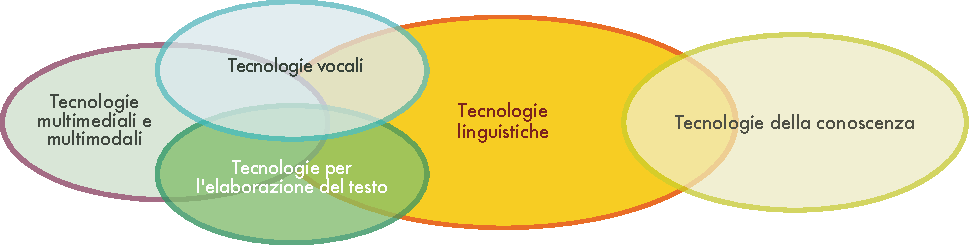
\includegraphics[width=\textwidth]{../_media/italian/language_technologies}
  \caption{Tecnologie linguistiche}
  \label{fig:ltincontext_de}
  \colorrule{grey3}{\textwidth}{1.5pt}
\end{figure*}

Quando comunichiamo, combiniamo il linguaggio con altri modi di comunicazione
e mezzi di informazione - per esempio il parlare pu\`{o} includere gesti ed
espressioni facciali. I testi digitali sono collegati a immagini e suoni. I
film possono contenere il linguaggio in forma parlata e scritta. In altre
parole, le tecnologie vocali e testuali si sovrappongono e interagiscono con
altre tecnologie della comunicazione multimodali e multimediali.

In questo capitolo, presenteremo i campi principali di applicazione delle
tecnologie linguistiche, ovvero il controllo ortografico e grammaticale di una
lingua, la ricerca su Web, la tecnologia vocale, e la traduzione automatica.
Queste applicazioni e tecnologie di base includono:

\begin{itemize}
\item correzione ortografica
\item supporto alla creazione di documenti
\item apprendimento linguistico assistito da computer
\item \emph{information retrieval}
\item estrazione di informazione
\item sommarizzazione automatica
\item \emph{question answering}
\item riconoscimento vocale 
\item sintesi vocale
\end{itemize}

L'area di ricerca relativa alle tecnologie del linguaggio dispone
di un vasto insieme di letteratura introduttiva; per un approfondimento 
si rimanda ai seguenti riferimenti bibliografici:  
\cite{carstensen-etal1, jurafsky-martin01, manning-schuetze1,  lt-world1, lt-survey1}.

Prima di discutere queste aree di applicazione, descriveremo brevemente
l'architettura di un tipico sistema di tecnologie del linguaggio.

\subsection{Architetture applicative}

Le applicazioni software per l'elaborazione del linguaggio generalmente sono
costituite da pi\`{u} componenti che rispecchiano i diversi aspetti del
linguaggio. Sebbene tali applicazioni siano tipicamente molto complesse, la 
Figura~\ref{fig:textprocessingarch_de} mostra un'architettura altamente 
semplificata di un tipico sistema di elaborazione del testo. I primi tre
moduli gestiscono la struttura e il significato del testo in ingresso:

\begin{enumerate}
\item \emph{Pre-processing}: prepara i dati, analizza o rimuove il formato, rileva la lingua in ingresso, rileva gli accenti (“citt\`{a}" e “citta'") e gli apostrofi (“dell'UE" e “della UE") per l'italiano, e cos\`{i} via.
\item Analisi grammaticale: riconosce il verbo, i suoi oggetti, modificatori e altre parti del discorso e inoltre rileva la struttura della frase.
\item Analisi semantica: esegue la disambiguazione (cio\`{e} calcola il significato appropriato delle parole in un dato contesto), risolve l'anafora (cio\`{e} quali pronomi si riferiscono a quali sostantivi nella frase) e le espressioni sostitutive, e rappresenta il significato della frase in un formato leggibile da una macchina.
\end{enumerate}

Dopo aver analizzato il testo, dei moduli specifici per un certo compito
possono eseguire altre operazioni, come il riassunto automatico e la ricerca
in un database.

Dopo aver introdotto le aree chiave della tecnologie linguistiche, 
nella parte restante di questo capitolo forniremo
prima una breve panoramica dello stato attuale della ricerca e della
formazione in questo campo e poi un quadro dei programmi di ricerca
passati e attuali. Infine, presenteremo una stima esperta degli
strumenti e delle risorse che sono fondamentali per l'italiano da diversi
punti di vista, quali la disponibilit\`{a}, la maturit\`{a} e la qualit\`{a}. 
La situazione generale delle tecnologie linguistiche per l'italiano \`{e} 
infine riassunta in Figura~\ref{fig:lrlttable_de} (p.~\pageref{fig:lrlttable_de}) alla fine di questo capitolo. Questa tabella elenca tutti gli strumenti e le risorse che sono \textbf{evidenziati} nel testo. Le tecnologie linguistiche per l'italiano sono confrontate anche con quelle per le altre lingue facenti parte di questa collana.



\begin{figure*}[htb]
  \colorrule{grey3}{\textwidth}{1.5pt}
  \center
  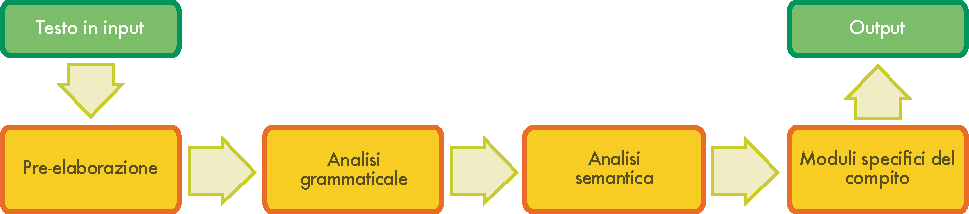
\includegraphics[width=\textwidth]{../_media/italian/text_processing_app_architecture}
  \caption{Architettura tipica di un'applicazione per l'elaborazione del testo}
  \label{fig:textprocessingarch_de}
  \colorrule{grey3}{\textwidth}{1.5pt}
\end{figure*}


\subsection{Ambiti applicativi principali} 

In questa sezione, ci concentriamo sugli strumenti e le risorse pi\`{u}
importanti per le tecnologie linguistiche, per poi passare ad una panoramica
delle attivit\`{a} legate alle tecnologie del linguaggio in Italia. 

\subsubsection{Controllo ortografico e \newline \mbox{grammaticale}}

Chiunque abbia usato un editore di testo come Microsoft Word sa che dispone di un correttore ortografico che evidenzia gli errori di ortografia e propone delle correzioni. I primi programmi di correzione ortografica confrontavano una lista di parole estratte con un dizionario di parole scritte correttamente. Oggi questi programmi sono molto pi\`{u} sofisticati. Utilizzando algoritmi dipendenti dalla lingua per l'\textbf{analisi grammaticale}, rilevano gli errori relativi alla morfologia (per esempio, la formazione del plurale), cos\`{i} come gli errori relativi alla sintassi, come un verbo mancante o un conflitto di accordo verbo-soggetto contratto (ad esempio, \emph{lei *scrivo una lettera}). Ma la maggior parte dei correttori ortografici non trover\`{a} alcun errore nel testo che segue \cite{zar1}:

\begin{itemize}
\item *Per salire in casa occorre fare 15 \emph{scali}
\item (Per salire in casa occorre fare 15 \emph{gradini})
\end{itemize}

La gestione di questo tipo di errori di solito richiede un'analisi del contesto.
Questo tipo di analisi deve attingere a delle \textbf{grammatiche} specifiche per una lingua, faticosamente codificate nel software da parte di esperti, o ad un modello di linguaggio statistico. In quest'ultimo caso, un modello calcola la probabilit\`{a} di una certa parola di comparire in una determinata posizione (ad esempio, tra le parole che la precedono e la seguono). Ad esempio: \emph{15 gradini} \`{e} una sequenza di parole pi\`{u} probabile di \emph{15 scali}. Un modello di linguaggio statistico pu\`{o} essere creato automaticamente utilizzando una grande quantit\`{a} di dati linguistici (corretti), un cosiddetto \textbf{corpus di testo}. La maggior parte di questi approcci sono stati sviluppati sulla base di dati per la lingua inglese. Nessuno dei due approcci pu\`{o} essere facilmente trasferito all'italiano perch\'{e} la lingua ha un ordine flessibile delle parole e un sistema flessionale pi\`{u} ricco.

Il controllo ortografico e grammaticale non \`{e} limitato agli editori di testo, ma \`{e} usato anche in “sistemi di supporto alla creazione di documenti", cio\`{e} ambienti software con cui sono scritti i manuali e altra documentazione che segue standard particolari per le tecnologie dell'informazione, i prodotti sanitari, l'ingegneria ed altro. Temendo lamentele da parte dei clienti circa l'uso scorretto e richieste di risarcimento per danni dovuti a istruzioni poco chiare, le aziende sono sempre pi\`{u} concentrate sulla qualit\`{a} della documentazione tecnica, puntando al contempo al mercato internazionale (tramite traduzione o localizzazione). I progressi nella elaborazione del linguaggio naturale hanno portato allo sviluppo di software di supporto alla creazione di documenti, che aiutano l'autore di documentazione tecnica nell'uso di un vocabolario e di una costruzione della frase coerenti con le regole del settore e con le restrizioni terminologiche aziendali.

\boxtext{L'uso del controllo ortografico e grammaticale non \`{e} limitato
  agli editori di testo ma \`{e} usato anche nei sistemi di supporto alla
  creazione di documenti.}

Oltre ai correttori ortografici e ai supporti alla creazione di documenti, il controllo grammaticale \`{e} importante anche nel campo dell'apprendimento delle lingue assistito da computer. Le applicazioni di controllo grammaticale correggono automaticamente le \emph{query} dei motori di ricerca, come ad esempio nei suggerimenti di Google.

%
\begin{figure*}[htb]
  \colorrule{grey3}{\textwidth}{1.5pt}
  \center
  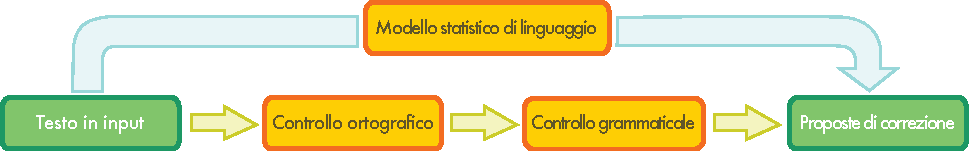
\includegraphics[width=\textwidth]{../_media/italian/language_checking}
  \caption{Correttore ortografico e grammaticale (sopra: statistica, sotto: a regole)}
  \label{fig:langcheckingaarch_de}
  \colorrule{grey3}{\textwidth}{1.5pt}
\end{figure*}

\subsubsection{Ricerca nel Web}

La ricerca nel Web, nelle intranet o nelle biblioteche digitali \`{e} probabilmente l'applicazione di tecnologia del linguaggio oggi pi\`{u} usata, anche se  in gran parte ancora poco sviluppata. Il motore di ricerca di Google, che ha iniziato nel 1998, gestisce oggi circa l'80\% di tutte le \emph{query} di ricerca \cite{spi1}. L'interfaccia di ricerca di Google e la pagina che mostra i risultati non sono significativamente cambiate rispetto alla prima versione. Tuttavia, nella versione attuale Google offre la correzione ortografica per le parole errate e di recente ha incorporato delle funzionalit\`{a} di base di ricerca semantica che possono migliorare la precisione della ricerca analizzando il significato dei termini in un dato contesto di \emph{query} di ricerca \cite{pc1}. La storia del successo di Google mostra che una grande quantit\`{a} di dati e delle tecniche di indicizzazione efficienti sono in grado di fornire risultati soddisfacenti usando un approccio basato sulla statistica.

\begin{figure*}[htb]
  \colorrule{grey3}{\textwidth}{1.5pt}
  \center
  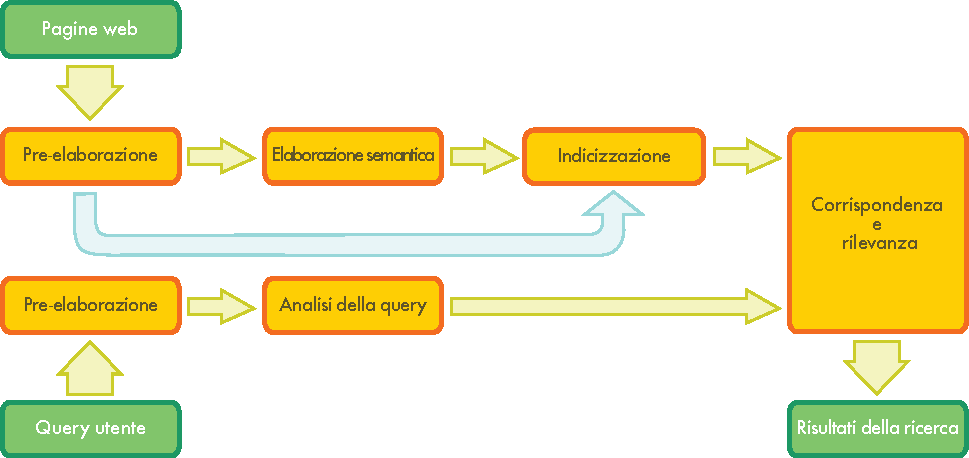
\includegraphics[width=\textwidth]{../_media/italian/web_search_architecture}
  \caption{Ricerca su Web}
  \label{fig:websearcharch_de}
  \colorrule{grey3}{\textwidth}{1.5pt}
\end{figure*}

Per richieste di informazioni pi\`{u} sofisticate, \`{e} essenziale integrare
delle conoscenze linguistiche pi\`{u} approfondite che consentano
l'interpretazione del testo. Esperimenti che hanno utilizzato delle
\textbf{risorse lessicali} come thesauri elettronici o risorse linguistiche
ontologiche (ad esempio, WordNet per l'inglese o ItalWordNet e MultiWordNet
per l'italiano) hanno dimostrato dei miglioramenti nella ricerca di pagine
utilizzando dei sinonimi dei termini di ricerca originali, come “energia"
atomica e “energia nucleare", o termini meno strettamente connessi.

La prossima generazione di motori di ricerca dovr\`{a} includere una
tecnologia linguistica molto pi\`{u} sofisticata, in particolare per
affrontare \emph{query} di ricerca costituite da domande o altri tipi di
frase, piuttosto che da un elenco di parole chiave. Per la richiesta \emph{Dammi un
elenco di tutte le aziende che sono state rilevate da altre societ\`{a} negli
ultimi cinque anni}, \`{e} necessaria un'\textbf{analisi semantica} oltre a quella sintattica. Il sistema dovr\`{a} inoltre fornire un indice per recuperare rapidamente i documenti rilevanti. Una risposta soddisfacente
richieder\`{a} l'analisi sintattica per analizzare la struttura grammaticale
della frase e determinare che l'utente desidera conoscere le aziende che sono
state acquisite, e non le societ\`{a} che hanno acquisito altre
societ\`{a}. Per l'espressione \emph{gli ultimi cinque anni}, il sistema deve
determinare gli anni in questione. E la \emph{query} deve essere confrontata
con una quantit\`{a} enorme di dati non strutturati per trovare la o le
informazioni pertinenti che l'utente desidera. Questo processo si chiama
\emph{information retrieval}, e implica la ricerca e la classificazione dei 
documenti rilevanti. Per generare un elenco di societ\`{a}, il sistema deve 
anche riconoscere che una particolare stringa di parole in un documento \`{e} 
il nome della societ\`{a}, utilizzando un processo chiamato “riconoscimento di entit\`{a}
nominate".

\boxtext{La prossima generazione di motori di ricerca dovr\`{a} includere una
  tecnologia linguistica molto pi\`{u} sofisticata.}

Una sfida ancora pi\`{u} impegnativa \`{e} far corrispondere una \emph{query}
in una lingua con dei documenti in un'altra lingua. Il \emph{cross-lingual
  information retrieval} comporta tradurre automaticamente la \emph{query} in
tutte le lingue di origine possibili e poi di nuovo tradurre i risultati nella
lingua di destinazione.

Ora che i dati sono sempre pi\`{u} disponibili in formati non testuali, sono
necessari dei servizi che offrano il recupero di informazione multimediale
attraverso la ricerca di immagini, file audio e dati video. Nel caso di file
audio e video, un modulo di riconoscimento vocale deve convertire il contenuto
parlato in testo (o in una rappresentazione fonetica) che possa poi essere
confrontato con una \emph{query} dell'utente.

In Italia, aziende come Expert System e CELI, tra gli altri, sviluppano e
applicano con successo le tecnologie di ricerca semantica.


\subsubsection{Interazione Vocale}

L'interazione vocale \`{e} una delle molte aree applicative che dipendono
dalle tecnologie vocali, ovvero quello tecnologie che consentono
l'elaborazione del linguaggio parlato. Le tecnologie per l'interazione vocale
sono utilizzate per creare interfacce che consentono agli utenti di interagire
in linguaggio parlato anzich\'{e} usare un display grafico, tastiera e
mouse. Oggi, queste interfacce utente vocali (\emph{Voice User Interfaces} -
VUI) vengono utilizzate per servizi telefonici completamente o parzialmente
automatizzati che vengono forniti dalle societ\`{a} ai clienti, ai dipendenti
o ai partner commerciali. I domini applicativi che si basano massicciamente
sulle VUI includono banche, catene di distribuzione, trasporti pubblici, e
telecomunicazioni. Altri usi delle tecnologie per l'interazione vocale
includono le interfacce dei sistemi di navigazione per auto e l'uso del
linguaggio parlato come alternativa alle interfacce grafiche o touch-screen
negli smartphone.

\boxtext{La tecnologia vocale rappresenta la base per creare delle interfacce
  che permettano ad un utente di interagire tramite il linguaggio parlato
  invece di uno schermo grafico, tastiera e mouse.}

\begin{figure*}[htb]
  \colorrule{grey3}{\textwidth}{1.5pt}
  \center 
  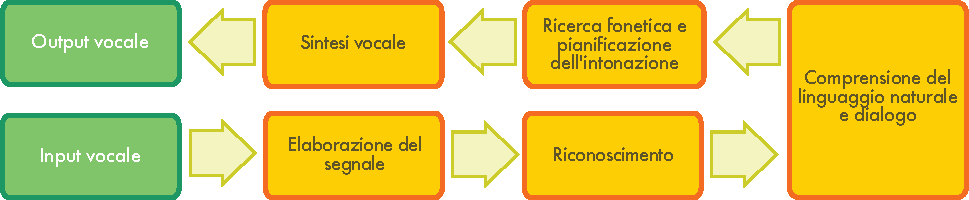
\includegraphics[width=\textwidth]{../_media/italian/simple_speech-based_dialogue_architecture}
  \caption{Sistema di dialogo parlato}
  \label{fig:dialoguearch_de}
  \colorrule{grey3}{\textwidth}{1.5pt}
\end{figure*}

L'interazione vocale comprende quattro tecnologie: 

\begin{enumerate}
\item Il \textbf{riconoscimento vocale} automatico (ASR), che determina quali parole sono effettivamente pronunciate in una data sequenza di suoni emessi da un utente.
\item La comprensione del linguaggio naturale analizza la struttura sintattica dell'espressione di un utente e la interpreta secondo il sistema in questione.
\item La gestione del dialogo determina l'azione da intraprendere in base all'input dell'utente e le funzionalit\`{a} del sistema.
\item La \textbf{sintesi vocale} (\emph{text-to-speech} o TTS) trasforma la risposta del sistema in suoni per l'utente.
\end{enumerate}

Una delle sfide principali dei sistemi di riconoscimento vocale consiste nel riconoscere con precisione le parole pronunciate da un utente. Questo significa limitare la gamma di espressioni possibili degli utenti ad un insieme limitato di parole chiave, oppure creare manualmente dei modelli di linguaggio che coprano una vasta gamma di espressioni in linguaggio naturale. Utilizzando tecniche di \emph{machine learning}, dei modelli di linguaggio possono essere generati anche automaticamente da \textbf{corpora di parlato}, ovvero grandi raccolte di file audio vocali e trascrizioni testuali. Limitare le espressioni di solito costringe le persone a utilizzare l'interfaccia utente vocale in modo rigido e pu\`{o} pregiudicare l'accettazione da parte dell'utente, ma la creazione, l'adattamento e la manutenzione di modelli di linguaggio ricchi aumentano sensibilmente i costi. Le interfacce vocali che utilizzano modelli linguistici e permettono inizialmente all'utente di esprimere le proprie intenzioni in modo pi\`{u} flessibile - per esempio tramite un saluto introduttivo come \emph{Come posso aiutarla?} - tendono ad essere automatizzate e sono accettate meglio dagli utenti.

Le aziende tendono ad usare delle espressioni pre-registrate da attori professionisti per generare l'output dell'interfaccia utente vocale. Per  espressioni statiche in cui la formulazione non dipende da contesti d'uso particolari o da dati personali, questo pu\`{o} offrire un'esperienza pi\`{u} ricca per l'utente. Tuttavia, i contenuti pi\`{u} dinamici in un enunciato potrebbero essere compromessi da un'intonazione innaturale derivante dalla semplice combinazione di frammenti di file audio. I sistemi di sintesi vocale attuali sono in continuo miglioramento (anche se possono essere ancora ottimizzati) nel produrre espressioni dinamiche che suonino naturali.

Nel mercato dell'interazione vocale le interfacce sono state notevolmente standardizzate negli ultimi dieci anni in termini di componenti tecnologici vari. C'\`{e} stato anche un forte consolidamento nel mercato del riconoscimento vocale e della sintesi vocale. I mercati nazionali dei paesi del G20 (paesi economicamente resilienti e intensamente popolati) sono stati dominati da sole cinque figure di livello mondiale, con Nuance (USA) e Loquendo (Italia) a rappresentare le figure pi\`{u} importanti in Europa. Nel 2011, Nuance ha completato l'acquisizione di Loquendo, definendo cos\`{i} un ulteriore passo avanti nel consolidamento del mercato.

Nel mercato del riconoscimento vocale automatico per la lingua italiana, ci sono anche aziende pi\`{u} piccole come PerVoice, Cedat85 e Synthema. Per quanto riguarda la tecnologia e il know-how della gestione del dialogo, il mercato \`{e} dominato da operatori nazionali per le PMI. In Italia, questi includono IM Service Lab. Piuttosto che fare affidamento su un modello produttivo basati su licenze software, queste aziende sono posizionate principalmente come fornitori di servizi completi che creano interfacce utente vocali come parte di un servizio di integrazione di sistema. Nel settore della tecnologia interattiva, non vi \`{e} ancora un vero mercato per tecnologie di base basate su analisi sintattica e semantica.

La domanda di interfacce utente vocali in Italia \`{e} cresciuta rapidamente negli ultimi cinque anni, trainata dalla richiesta crescente per servizi self-service da parte dei clienti, per un'ottimizzazione dei costi per servizi telefonici automatizzati, e dalla crescente accettazione del linguaggio parlato come mezzo per interazione uomo-macchina.

Guardando al futuro, ci saranno cambiamenti significativi dovuti alla diffusione degli smartphone quale nuova piattaforma per la gestione delle relazioni con i clienti in aggiunta ai telefoni fissi, Internet e posta elettronica. Questo influir\`{a} anche sul modo in cui \`{e} usata la tecnologia vocale. Nel lungo periodo, ci sar\`{a} un minor numero di interfacce vocali basate sul telefono e il linguaggio parlato avr\`{a} un ruolo molto pi\`{u} centrale di accesso per gli smartphone. Questo sar\`{a} in gran parte determinato dai miglioramenti intervenuti nell'accuratezza del riconoscimento vocale indipendente dal parlante attraverso i servizi di dettatura vocale gi\`{a} offerti come servizi centralizzati agli utenti di smartphone.


\subsubsection{Traduzione automatica}


\begin{figure*}[htb]
  \colorrule{grey3}{\textwidth}{1.5pt}
  \center
  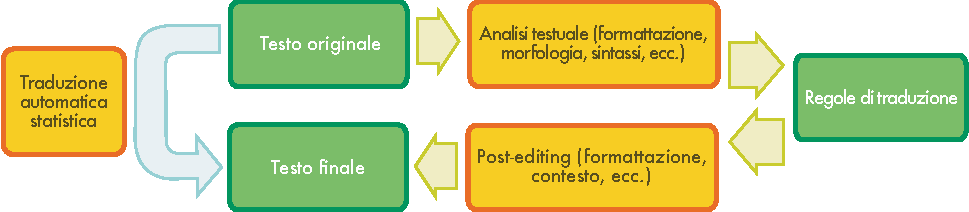
\includegraphics[width=\textwidth]{../_media/italian/machine_translation}
  \caption{Traduzione automatica  (a sinistra: statistico, a destra: a regole)}
  \label{fig:mtarch_de}
  \colorrule{grey3}{\textwidth}{1.5pt}
\end{figure*}

L'idea di utilizzare i computer per tradurre le lingue naturali risale al 1946 ed \`{e} stata seguita da cospicui finanziamenti per la ricerca durante gli anni '50 e nuovamente negli anni '80. Eppure la \textbf{traduzione automatica} (\emph{Machine Translation}, MT) non \`{e} ancora in grado di mantenere la sua promessa iniziale.

Nella traduzione automatica, l'approccio pi\`{u} semplice consiste nel
sostituire automaticamente le parole di un testo in una certa lingua
naturale con parole in un'altra lingua. Questo pu\`{o} essere utile in
ambiti che hanno un linguaggio molto limitato e stereotipato, come le
previsioni meteo. Ma per produrre una buona traduzione di testi meno
standardizzati, per unit\`{a} di testo pi\`{u} grandi (sintagmi, frasi
o anche interi passaggi), devono essere trovati gli omologhi migliori
nella lingua di arrivo. 

\boxtext{Ad un livello base, la traduzione automatica consiste semplicemente
  nella sostituzione di parole in una lingua con parole in un'altra lingua.}

La difficolt\`{a} maggiore \`{e} che il linguaggio umano \`{e} ambiguo. L'ambiguit\`{a} crea problemi su pi\`{u} livelli, ad esempio il livello lessicale (la parola inglese \emph{jaguar} pu\`{o} essere tradotta come una marca di auto o come un animale) o il livello sintattico, per esempio:

\begin{itemize}
\item The chicken is ready \emph{to eat}.
\item {[}Il pollo  \`{e} pronto \emph{a mangiare}.{]}
\item {[}Il pollo  \`{e} pronto \emph{per essere mangiato}.{]}
\end{itemize}

Un modo di costruire un sistema di MT consiste nell'utilizzare delle regole linguistiche. Per le traduzioni tra lingue molto simili, una traduzione diretta basata sulla sostituzione pu\`{o} essere fattibile in casi come quello dell'esempio precedente. Tuttavia, i sistemi basati su regole (o basati sulla conoscenza linguistica) spesso analizzano il testo in input e creano una rappresentazione simbolica intermedia da cui il testo pu\`{o} essere generato nella lingua di destinazione. Il successo di questi metodi \`{e} fortemente dipendente dalla disponibilit\`{a} di grandi lessici dotati di informazioni morfologiche, sintattiche e semantiche, e di grandi insiemi di regole grammaticali attentamente progettate da linguisti esperti. Questo \`{e} un processo molto lungo e di conseguenza costoso.

L'interesse per i modelli statistici nella traduzione automatica \`{e} cresciuto verso la fine degli anni '80, quando la potenza di calcolo \`{e} aumentata ed \`{e} diventata meno costosa. I modelli statistici sono derivati dall'analisi di corpora testuali bilingui, come il \textbf{corpus parallelo} Europarl, che raccoglie gli atti del Parlamento europeo in 21 lingue europee. Con una quantit\`{a} sufficiente di dati, la traduzione automatica statistica funziona abbastanza bene da ricavare un significato approssimativo di un testo in una lingua straniera, elaborando versioni parallele e trovando delle sequenze di parole plausibili. Ma a differenza dei sistemi basati sulla conoscenza, la traduzione automatica statistica (o \emph{data-driven}) spesso genera un risultato sgrammaticato. La traduzione automatica \emph{data-driven} \`{e} vantaggiosa perch\'{e} richiede uno sforzo umano minore, e pu\`{o} anche trattare particolarit\`{a} speciali del linguaggio (ad esempio, le espressioni idiomatiche) che possono essere ignorate da sistemi basati sulla conoscenza.

I punti di forza e di debolezza della traduzione automatica basata sulla conoscenza e di quella \emph{data-driven} tendono ad essere complementari, di modo che al giorno d'oggi i ricercatori si concentrano su approcci ibridi che combinano entrambe le metodologie. Un approccio particolare utilizza sia sistemi basati sulla conoscenza che \emph{data-driven}, con un modulo di selezione che decide la migliore uscita per ogni frase. Tuttavia, i risultati per frasi pi\`{u} lunghe di 12 parole saranno spesso ben lontani dall'essere perfetti. Una soluzione pi\`{u} soddisfacente consiste nel combinare le parti migliori di ogni frase da pi\`{u} uscite diverse; la cosa pu\`{o} essere piuttosto complessa, in quanto non \`{e} sempre evidente quali siano le parti corrispondenti di alternative multiple, che devono essere allineate.

\boxtext{La traduzione automatica \`{e} particolarmente impegnativa per la
  lingua italiana.} 

La traduzione automatica \`{e} particolarmente impegnativa per la lingua italiana, che \`{e} morfologicamente complessa ed ha un ordine libero delle parole nella frase. Ci sono alcune aziende in Italia attive nel settore della traduzione automatica, soprattutto nella fornitura di servizi per usi professionali (ad esempio, Translated).

L'uso della traduzione automatica pu\`{o} aumentare la produttivit\`{a} in modo significativo, ammesso che il sistema sia adattato in modo intelligente alla terminologia specifica per l'utente e integrato nel flusso di lavoro. Sono stati sviluppati dei sistemi speciali per supportare la traduzione interattiva.

Il potenziale di miglioramento della qualit\`{a} dei sistemi di traduzione automatica \`{e} ancora enorme. Le sfide attuali riguardano l'adattamento delle risorse linguistiche a un dominio o argomento determinato e l'integrazione della tecnologia nei flussi di lavoro che dispongono gi\`{a} di database di termini e memorie di traduzione. Un altro problema \`{e} che la maggior parte dei sistemi attuali sono incentrati sull'inglese e supportano solo alcune lingue da e verso l'italiano. Questo comporta una frizione nel flusso di lavoro di traduzione e costringe gli utenti dei sistemi di traduzione automatica ad apprendere l'uso di strumenti diversi di codifica dei lessici per sistemi diversi.

\begin{figure*}[htbp]
  \centering
  \setlength{\tabcolsep}{0.17em}
  \small
  \begin{tabular}{>{\columncolor{corange1}}cccccccccccccccccccccccc}
    & \multicolumn{22}{>{\columncolor{corange1}}c}{Lingua target -- \textcolor{grey1}{Target language}}\\\addlinespace[{-.009cm}]
    \rowcolor{corange1}  & EN & BG & DE & CS & DA & EL & ES & ET & FI & FR & HU & IT & LT & LV & MT & NL & PL & PT & RO & SK & SL & SV\\
    EN & -- & \textcolor{blue}{40.5} & \textcolor{blue}{46.8} & \textcolor{green2}{52.6} & \textcolor{green2}{50.0} & \textcolor{blue}{41.0} & \textcolor{green2}{55.2} & \textcolor{purple}{34.8} & \textcolor{purple}{38.6} & \textcolor{green2}{50.1} & \textcolor{purple}{37.2} & \textcolor{green2}{50.4} & \textcolor{purple}{39.6} & \textcolor{blue}{43.4} & \textcolor{purple}{39.8} & \textcolor{green2}{52.3} & \textcolor{blue}{49.2} & \textcolor{green2}{55.0} & \textcolor{blue}{49.0} & \textcolor{blue}{44.7} & \textcolor{green2}{50.7} & \textcolor{green2}{52.0}\\
    BG & \textcolor{green}{61.3} & -- & \textcolor{purple}{38.7} & \textcolor{purple}{39.4} & \textcolor{purple}{39.6} & \textcolor{purple}{34.5} & \textcolor{blue}{46.9} & \textcolor{red3}{25.5} & \textcolor{red3}{26.7} & \textcolor{blue}{42.4} & \textcolor{red3}{22.0} & \textcolor{blue}{43.5} & \textcolor{red3}{29.3} & \textcolor{red3}{29.1} & \textcolor{red3}{25.9} & \textcolor{blue}{44.9} & \textcolor{purple}{35.1} & \textcolor{blue}{45.9} & \textcolor{purple}{36.8} & \textcolor{purple}{34.1} & \textcolor{purple}{34.1} & \textcolor{purple}{39.9}\\
    DE & \textcolor{green2}{53.6} & \textcolor{red3}{26.3} & -- & \textcolor{purple}{35.4} & \textcolor{blue}{43.1} & \textcolor{purple}{32.8} & \textcolor{blue}{47.1} & \textcolor{red3}{26.7} & \textcolor{red3}{29.5} & \textcolor{purple}{39.4} & \textcolor{red3}{27.6} & \textcolor{blue}{42.7} & \textcolor{red3}{27.6} & \textcolor{purple}{30.3} & \textcolor{red2}{19.8} & \textcolor{green2}{50.2} & \textcolor{purple}{30.2} & \textcolor{blue}{44.1} & \textcolor{purple}{30.7} & \textcolor{red3}{29.4} & \textcolor{purple}{31.4} & \textcolor{blue}{41.2}\\
    CS & \textcolor{green2}{58.4} & \textcolor{purple}{32.0} & \textcolor{blue}{42.6} & -- & \textcolor{blue}{43.6} & \textcolor{purple}{34.6} & \textcolor{blue}{48.9} & \textcolor{purple}{30.7} & \textcolor{purple}{30.5} & \textcolor{blue}{41.6} & \textcolor{red3}{27.4} & \textcolor{blue}{44.3} & \textcolor{purple}{34.5} & \textcolor{purple}{35.8} & \textcolor{red3}{26.3} & \textcolor{blue}{46.5} & \textcolor{purple}{39.2} & \textcolor{blue}{45.7} & \textcolor{purple}{36.5} & \textcolor{blue}{43.6} & \textcolor{blue}{41.3} & \textcolor{blue}{42.9}\\
    DA & \textcolor{green2}{57.6} & \textcolor{red3}{28.7} & \textcolor{blue}{44.1} & \textcolor{purple}{35.7} & -- & \textcolor{purple}{34.3} & \textcolor{blue}{47.5} & \textcolor{red3}{27.8} & \textcolor{purple}{31.6} & \textcolor{blue}{41.3} & \textcolor{red3}{24.2} & \textcolor{blue}{43.8} & \textcolor{red3}{29.7} & \textcolor{purple}{32.9} & \textcolor{red3}{21.1} & \textcolor{blue}{48.5} & \textcolor{purple}{34.3} & \textcolor{blue}{45.4} & \textcolor{purple}{33.9} & \textcolor{purple}{33.0} & \textcolor{purple}{36.2} & \textcolor{blue}{47.2}\\
    EL & \textcolor{green2}{59.5} & \textcolor{purple}{32.4} & \textcolor{blue}{43.1} & \textcolor{purple}{37.7} & \textcolor{blue}{44.5} & -- & \textcolor{green2}{54.0} & \textcolor{red3}{26.5} & \textcolor{red3}{29.0} & \textcolor{blue}{48.3} & \textcolor{red3}{23.7} & \textcolor{blue}{49.6} & \textcolor{red3}{29.0} & \textcolor{purple}{32.6} & \textcolor{red3}{23.8} & \textcolor{blue}{48.9} & \textcolor{purple}{34.2} & \textcolor{green2}{52.5} & \textcolor{purple}{37.2} & \textcolor{purple}{33.1} & \textcolor{purple}{36.3} & \textcolor{blue}{43.3}\\
    ES & \textcolor{green}{60.0} & \textcolor{purple}{31.1} & \textcolor{blue}{42.7} & \textcolor{purple}{37.5} & \textcolor{blue}{44.4} & \textcolor{purple}{39.4} & -- & \textcolor{red3}{25.4} & \textcolor{red3}{28.5} & \textcolor{green2}{51.3} & \textcolor{red3}{24.0} & \textcolor{green2}{51.7} & \textcolor{red3}{26.8} & \textcolor{purple}{30.5} & \textcolor{red3}{24.6} & \textcolor{blue}{48.8} & \textcolor{purple}{33.9} & \textcolor{green2}{57.3} & \textcolor{purple}{38.1} & \textcolor{purple}{31.7} & \textcolor{purple}{33.9} & \textcolor{blue}{43.7}\\
    ET & \textcolor{green2}{52.0} & \textcolor{red3}{24.6} & \textcolor{purple}{37.3} & \textcolor{purple}{35.2} & \textcolor{purple}{37.8} & \textcolor{red3}{28.2} & \textcolor{blue}{40.4} & -- & \textcolor{purple}{37.7} & \textcolor{purple}{33.4} & \textcolor{purple}{30.9} & \textcolor{purple}{37.0} & \textcolor{purple}{35.0} & \textcolor{purple}{36.9} & \textcolor{red3}{20.5} & \textcolor{blue}{41.3} & \textcolor{purple}{32.0} & \textcolor{purple}{37.8} & \textcolor{red3}{28.0} & \textcolor{purple}{30.6} & \textcolor{purple}{32.9} & \textcolor{purple}{37.3}\\
    FI & \textcolor{blue}{49.3} & \textcolor{red3}{23.2} & \textcolor{purple}{36.0} & \textcolor{purple}{32.0} & \textcolor{purple}{37.9} & \textcolor{red3}{27.2} & \textcolor{purple}{39.7} & \textcolor{purple}{34.9} & -- & \textcolor{red3}{29.5} & \textcolor{red3}{27.2} & \textcolor{purple}{36.6} & \textcolor{purple}{30.5} & \textcolor{purple}{32.5} & \textcolor{red2}{19.4} & \textcolor{blue}{40.6} & \textcolor{red3}{28.8} & \textcolor{purple}{37.5} & \textcolor{red3}{26.5} & \textcolor{red3}{27.3} & \textcolor{red3}{28.2} & \textcolor{purple}{37.6}\\
    FR & \textcolor{green}{64.0} & \textcolor{purple}{34.5} & \textcolor{blue}{45.1} & \textcolor{purple}{39.5} & \textcolor{blue}{47.4} & \textcolor{blue}{42.8} & \textcolor{green}{60.9} & \textcolor{red3}{26.7} & \textcolor{purple}{30.0} & -- & \textcolor{red3}{25.5} & \textcolor{green2}{56.1} & \textcolor{red3}{28.3} & \textcolor{purple}{31.9} & \textcolor{red3}{25.3} & \textcolor{green2}{51.6} & \textcolor{purple}{35.7} & \textcolor{green}{61.0} & \textcolor{blue}{43.8} & \textcolor{purple}{33.1} & \textcolor{purple}{35.6} & \textcolor{blue}{45.8}\\
    HU & \textcolor{blue}{48.0} & \textcolor{red3}{24.7} & \textcolor{purple}{34.3} & \textcolor{purple}{30.0} & \textcolor{purple}{33.0} & \textcolor{red3}{25.5} & \textcolor{purple}{34.1} & \textcolor{red3}{29.6} & \textcolor{red3}{29.4} & \textcolor{purple}{30.7} & -- & \textcolor{purple}{33.5} & \textcolor{red3}{29.6} & \textcolor{purple}{31.9} & \textcolor{red2}{18.1} & \textcolor{purple}{36.1} & \textcolor{red3}{29.8} & \textcolor{purple}{34.2} & \textcolor{red3}{25.7} & \textcolor{red3}{25.6} & \textcolor{red3}{28.2} & \textcolor{purple}{30.5}\\
    IT & \textcolor{green}{61.0} & \textcolor{purple}{32.1} & \textcolor{blue}{44.3} & \textcolor{purple}{38.9} & \textcolor{blue}{45.8} & \textcolor{blue}{40.6} & \textcolor{red3}{26.9} & \textcolor{red3}{25.0} & \textcolor{red3}{29.7} & \textcolor{green2}{52.7} & \textcolor{red3}{24.2} & -- & \textcolor{red3}{29.4} & \textcolor{purple}{32.6} & \textcolor{red3}{24.6} & \textcolor{green2}{50.5} & \textcolor{purple}{35.2} & \textcolor{green2}{56.5} & \textcolor{purple}{39.3} & \textcolor{purple}{32.5} & \textcolor{purple}{34.7} & \textcolor{blue}{44.3}\\
    LT & \textcolor{green2}{51.8} & \textcolor{red3}{27.6} & \textcolor{purple}{33.9} & \textcolor{purple}{37.0} & \textcolor{purple}{36.8} & \textcolor{red3}{26.5} & \textcolor{red3}{21.1} & \textcolor{purple}{34.2} & \textcolor{purple}{32.0} & \textcolor{purple}{34.4} & \textcolor{red3}{28.5} & \textcolor{purple}{36.8} & -- & \textcolor{blue}{40.1} & \textcolor{red3}{22.2} & \textcolor{purple}{38.1} & \textcolor{purple}{31.6} & \textcolor{purple}{31.6} & \textcolor{red3}{29.3} & \textcolor{purple}{31.8} & \textcolor{purple}{35.3} & \textcolor{purple}{35.3}\\
    LV & \textcolor{green2}{54.0} & \textcolor{red3}{29.1} & \textcolor{purple}{35.0} & \textcolor{purple}{37.8} & \textcolor{purple}{38.5} & \textcolor{red3}{29.7} & \textcolor{red2}{8.0} & \textcolor{purple}{34.2} & \textcolor{purple}{32.4} & \textcolor{purple}{35.6} & \textcolor{red3}{29.3} & \textcolor{purple}{38.9} & \textcolor{purple}{38.4} & -- & \textcolor{red3}{23.3} & \textcolor{blue}{41.5} & \textcolor{purple}{34.4} & \textcolor{purple}{39.6} & \textcolor{purple}{31.0} & \textcolor{purple}{33.3} & \textcolor{purple}{37.1} & \textcolor{purple}{38.0}\\
    MT & \textcolor{green}{72.1} & \textcolor{purple}{32.2} & \textcolor{purple}{37.2} & \textcolor{purple}{37.9} & \textcolor{purple}{38.9} & \textcolor{purple}{33.7} & \textcolor{blue}{48.7} & \textcolor{red3}{26.9} & \textcolor{red3}{25.8} & \textcolor{blue}{42.4} & \textcolor{red3}{22.4} & \textcolor{blue}{43.7} & \textcolor{purple}{30.2} & \textcolor{purple}{33.2} & -- & \textcolor{blue}{44.0} & \textcolor{purple}{37.1} & \textcolor{blue}{45.9} & \textcolor{purple}{38.9} & \textcolor{purple}{35.8} & \textcolor{blue}{40.0} & \textcolor{blue}{41.6}\\
    NL & \textcolor{green2}{56.9} & \textcolor{red3}{29.3} & \textcolor{blue}{46.9} & \textcolor{purple}{37.0} & \textcolor{blue}{45.4} & \textcolor{purple}{35.3} & \textcolor{blue}{49.7} & \textcolor{red3}{27.5} & \textcolor{red3}{29.8} & \textcolor{blue}{43.4} & \textcolor{red3}{25.3} & \textcolor{blue}{44.5} & \textcolor{red3}{28.6} & \textcolor{purple}{31.7} & \textcolor{red3}{22.0} & -- & \textcolor{purple}{32.0} & \textcolor{blue}{47.7} & \textcolor{purple}{33.0} & \textcolor{purple}{30.1} & \textcolor{purple}{34.6} & \textcolor{blue}{43.6}\\
    PL & \textcolor{green}{60.8} & \textcolor{purple}{31.5} & \textcolor{blue}{40.2} & \textcolor{blue}{44.2} & \textcolor{blue}{42.1} & \textcolor{purple}{34.2} & \textcolor{blue}{46.2} & \textcolor{red3}{29.2} & \textcolor{red3}{29.0} & \textcolor{blue}{40.0} & \textcolor{red3}{24.5} & \textcolor{blue}{43.2} & \textcolor{purple}{33.2} & \textcolor{purple}{35.6} & \textcolor{red3}{27.9} & \textcolor{blue}{44.8} & -- & \textcolor{blue}{44.1} & \textcolor{purple}{38.2} & \textcolor{purple}{38.2} & \textcolor{purple}{39.8} & \textcolor{blue}{42.1}\\
    PT & \textcolor{green}{60.7} & \textcolor{purple}{31.4} & \textcolor{blue}{42.9} & \textcolor{purple}{38.4} & \textcolor{blue}{42.8} & \textcolor{blue}{40.2} & \textcolor{green}{60.7} & \textcolor{red3}{26.4} & \textcolor{red3}{29.2} & \textcolor{green2}{53.2} & \textcolor{red3}{23.8} & \textcolor{green2}{52.8} & \textcolor{red3}{28.0} & \textcolor{purple}{31.5} & \textcolor{red3}{24.8} & \textcolor{blue}{49.3} & \textcolor{purple}{34.5} & -- & \textcolor{purple}{39.4} & \textcolor{purple}{32.1} & \textcolor{purple}{34.4} & \textcolor{blue}{43.9}\\
    RO & \textcolor{green}{60.8} & \textcolor{purple}{33.1} & \textcolor{purple}{38.5} & \textcolor{purple}{37.8} & \textcolor{blue}{40.3} & \textcolor{purple}{35.6} & \textcolor{green2}{50.4} & \textcolor{red3}{24.6} & \textcolor{red3}{26.2} & \textcolor{blue}{46.5} & \textcolor{red3}{25.0} & \textcolor{blue}{44.8} & \textcolor{red3}{28.4} & \textcolor{red3}{29.9} & \textcolor{red3}{28.7} & \textcolor{blue}{43.0} & \textcolor{purple}{35.8} & \textcolor{blue}{48.5} & -- & \textcolor{purple}{31.5} & \textcolor{purple}{35.1} & \textcolor{purple}{39.4}\\
    SK & \textcolor{green}{60.8} & \textcolor{purple}{32.6} & \textcolor{purple}{39.4} & \textcolor{blue}{48.1} & \textcolor{blue}{41.0} & \textcolor{purple}{33.3} & \textcolor{blue}{46.2} & \textcolor{red3}{29.8} & \textcolor{red3}{28.4} & \textcolor{purple}{39.4} & \textcolor{red3}{27.4} & \textcolor{blue}{41.8} & \textcolor{purple}{33.8} & \textcolor{purple}{36.7} & \textcolor{red3}{28.5} & \textcolor{blue}{44.4} & \textcolor{purple}{39.0} & \textcolor{blue}{43.3} & \textcolor{purple}{35.3} & -- & \textcolor{blue}{42.6} & \textcolor{blue}{41.8}\\
    SL & \textcolor{green}{61.0} & \textcolor{purple}{33.1} & \textcolor{purple}{37.9} & \textcolor{blue}{43.5} & \textcolor{blue}{42.6} & \textcolor{purple}{34.0} & \textcolor{blue}{47.0} & \textcolor{purple}{31.1} & \textcolor{red3}{28.8} & \textcolor{purple}{38.2} & \textcolor{red3}{25.7} & \textcolor{blue}{42.3} & \textcolor{purple}{34.6} & \textcolor{purple}{37.3} & \textcolor{purple}{30.0} & \textcolor{blue}{45.9} & \textcolor{purple}{38.2} & \textcolor{blue}{44.1} & \textcolor{purple}{35.8} & \textcolor{purple}{38.9} & -- & \textcolor{blue}{42.7}\\
    SV & \textcolor{green2}{58.5} & \textcolor{red3}{26.9} & \textcolor{blue}{41.0} & \textcolor{purple}{35.6} & \textcolor{blue}{46.6} & \textcolor{purple}{33.3} & \textcolor{blue}{46.6} & \textcolor{red3}{27.4} & \textcolor{purple}{30.9} & \textcolor{purple}{38.9} & \textcolor{red3}{22.7} & \textcolor{blue}{42.0} & \textcolor{red3}{28.2} & \textcolor{purple}{31.0} & \textcolor{red3}{23.7} & \textcolor{blue}{45.6} & \textcolor{purple}{32.2} & \textcolor{blue}{44.2} & \textcolor{purple}{32.7} & \textcolor{purple}{31.3} & \textcolor{purple}{33.5} & --\\
    \end{tabular}
  \caption{Traduzione automatica tra 22 lingue dell'UE -- \textcolor{grey1}{Machine translation between 22 EU-languages\cite{euro1}}}
  \label{fig:euromatrix_de}
\end{figure*}

Le campagne di valutazione aiutano a confrontare la qualit\`{a} dei sistemi di
traduzione automatica, i diversi approcci e lo stato dei sistemi per coppie di
lingue diverse. La Figura~\ref{fig:euromatrix_de}
(p.~\pageref{fig:euromatrix_de}), che \`{e} stata preparata durante il progetto europeo Euromatrix +, mostra le prestazioni ottenute per coppie di
lingue su 22 delle 23 lingue ufficiali dell'UE (l'irlandese non \`{e} stato
confrontato). I risultati sono classificati in base al punteggio BLEU, che
assegna punteggi pi\`{u} alti alle traduzioni migliori \cite{bleu1} (un traduttore umano
raggiungerebbe un punteggio di circa 80 punti).

I risultati migliori (in verde e blu) sono stati raggiunti da quelle lingue che beneficiano di un notevole sforzo di ricerca in programmi coordinati e dell'esistenza di molti corpora paralleli (ad esempio, inglese, francese, olandese, spagnolo e tedesco). Le lingue con risultati inferiori sono contrassegnate in rosso. Per queste  lingue o mancano sforzi di sviluppo analoghi o sono strutturalmente molto diverse dalle altre lingue (ad esempio, ungherese, maltese e finlandese).


% -- \textcolor{grey1}{Machine translation between 22 EU-languages} 

\subsection{Altre aree applicative}

La creazione di applicazioni di tecnologia linguistica comporta una serie di
attivit\`{a} secondarie che non sempre affiorano al livello di interazione con
l'utente, ma forniscono funzionalit\`{a} di servizio cruciali del
sistema in questione. Tutte rappresentano importanti temi di ricerca che
ora si sono evoluti in sotto-discipline indipendenti della linguistica
computazionale. Il \emph{question answering}, per esempio, \`{e} un'area di ricerca molto attiva, per la quale sono stati costruiti dei corpora annotati e sono state avviate delle competizioni scientifiche. L'idea alla base del \emph{question answering} \`{e} di andare oltre la ricerca basata su parole chiave (in cui il motore di ricerca risponde fornendo una raccolta di documenti potenzialmente rilevanti) e consentire agli utenti di fare una domanda concreta a cui il sistema fornisce una sola risposta. Per esempio:

\begin{itemize}
\item[] \textit{Domanda: Quanti anni aveva Neil Armstrong quando and\`{o} sulla luna?}
\item[] \textit{Risposta: 38.}
\end{itemize}

Anche se il \emph{question answering} \`{e} ovviamente correlato al settore della ricerca sul web, oggi \`{e} considerato un termine generico che ricomprende temi di ricerca quali i diversi tipi di domande possibili e come dovrebbero essere trattati, il modo di analizzare e confrontare un insieme di documenti che potenzialmente contengono la risposta (forniscono risposte contraddittorie?), e il modo per estrarre in modo attendibile delle informazioni specifiche (la risposta) da un documento senza ignorare il contesto.

\boxtext{Le applicazioni di tecnologia linguistica spesso forniscono delle
  funzionalit\`{a} di servizio importanti ricomprese in sistemi software pi\`{u} ampi.}

Il \emph{question answering} \`{e} a sua volta connesso con l'estrazione di informazioni (\emph{information extraction}, IE), un settore estremamente popolare ed influente al momento della svolta statistica della linguistica computazionale, nei primi anni '90. L' \emph{information extraction} si propone di identificare delle informazioni specifiche in specifiche classi di documenti, come ad esempio identificare gli attori-chiave in acquisizioni aziendali riportate in articoli di giornale. Un altro scenario comune che \`{e} stato studiato sono i rapporti sugli incidenti terroristici. Qui il problema consiste nel far coincidere il testo con un modello che specifica l'autore, l'obiettivo, l'ora, il luogo e i risultati dell'incidente. Il riempimento di modelli calibrato su un dominio specifico \`{e} la caratteristica centrale dell'\emph{information extraction}, il che la rende un altro esempio di tecnologia “dietro le quinte" che forma una ben delimitata area di ricerca che in pratica ha bisogno di essere integrata in un ambiente applicativo adatto.
La sommarizzazione automatica e la \textbf{generazione di testo} sono due aree di confine che possono agire sia come applicazioni indipendenti o giocare un ruolo di supporto. La sommarizzazione tenta di presentare gli elementi essenziali di un testo lungo in forma abbreviata, ed \`{e} una delle funzionalit\`{a} disponibili in Microsoft Word. Si utilizza per lo pi\`{u} un approccio statistico per identificare le parole “importanti" in un testo (per esempio, parole che compaiono molto di frequente nel testo in questione, ma meno di frequente nell'uso generale) e determinare quali frasi contengono la maggior parte di queste parole “importanti". Queste frasi vengono poi estratte e messe insieme per creare il riassunto. In questo scenario commerciale molto comune, la sommarizzazione \`{e} semplicemente una forma di estrazione di frasi, e il testo \`{e} ridotto a un sottoinsieme delle sue frasi. Un approccio alternativo, per il quale sono state svolte alcune ricerche, consiste nel generare frasi nuove, che non esistono nel testo di partenza. Questo richiede una comprensione pi\`{u} profonda del testo, il che significa che fino ad ora questo approccio \`{e} molto meno robusto. Nel complesso, un generatore di testo viene raramente utilizzato come applicazione indipendente, ma \`{e} inserito in un ambiente software pi\`{u} ampio, come ad esempio un sistema informativo clinico che raccoglie, memorizza ed elabora i dati dei pazienti. La creazione di rapporti \`{e} solo una delle molte applicazioni della sommarizzazione automatica.

\boxtext{Per la lingua italiana la ricerca nelle tecnologie di testo descritte \`{e} molto meno sviluppata  che per la lingua inglese.} 

La ricerca nelle tecnologie di testo descritte \`{e} molto meno sviluppata per la lingua italiana che per la lingua inglese. \emph{Question answering}, \emph{information extraction} e sommarizzazione automatica sono stati al centro di numerose competizioni negli Stati Uniti dal 1990, principalmente organizzate da organizzazioni governative quali DARPA e NIST. Queste competizioni hanno notevolmente migliorato lo stato dell'arte, ma la loro attenzione \`{e} stata principalmente sulla lingua inglese. Come risultato, in italiano ci sono meno corpora annotati o altre risorse speciali necessarie per svolgere questi compiti. I sistemi di sommarizzazione basati su  metodi puramente statistici sono in gran parte indipendenti dalla lingua e sono disponibili alcuni prototipi di ricerca. Per la generazione del testo, i componenti riutilizzabili sono tradizionalmente limitati ai moduli di realizzazione superficiale (grammatiche di generazione) e la maggior parte del software disponibile \`{e} per la lingua inglese.

\subsection{Programmi formativi}

Le tecnologie linguistiche costituiscono un campo altamente interdisciplinare che include le competenze combinate, fra gli altri, di linguisti, informatici, matematici, filosofi, psicolinguisti e neuroscienziati. Di conseguenza, questo campo di studi non ha acquisito una esistenza chiara e indipendente nel sistema universitario italiano.

Per quanto concerne i curricula universitari, segnaliamo il “Master Internazionale di secondo livello in Tecnologie del Linguaggio Umano e Interfacce” presso l'Universit\`{a} di Trento e il “Master Europeo in Tecnologie del Linguaggio e della Comunicazione” presso la Libera Universit\`{a} di Bolzano. Inoltre, secondo il “Libro Bianco”, a livello di laurea e di dottorato di ricerca sono attivi almeno altri 16 curricula collegati alle tecnologie del linguaggio (in particolare presso le Universit\`{a} di Venezia, Torino, Pavia, Pisa, Roma “Tor Vergata”, Napoli e Bari), per un totale di almeno 76 corsi universitari riguardanti questo campo in Italia, includendo quelli che fanno riferimento a percorsi di Informatica Umanistica.

\subsection{Progetti e iniziative nazionali}

La presenza “digitale” di una lingua in applicazioni e servizi basati su Internet \`{e} ormai un elemento cruciale per mantenere la vitalit\`{a} culturale di quella lingua. E, d'altra parte, applicazioni e servizi su Internet sono sostenibili solo in presenza di adeguate infrastrutture e tecnologie. Per quanto riguarda l'italiano, sebbene la situazione non possa essere paragonata a quella dell'inglese, a partire dal 1997 \`{e} stato fatto uno sforzo considerevole in Italia nella ricerca sulle tecnologie del linguaggio, quando per questo settore \`{e} stata designata una politica di ricerca nazionale con il lancio di due progetti della durata di tre anni:

\begin{itemize}
\item TAL, Infrastruttura Nazionale per le risorse Linguistiche nel campo del Trattamento Automatico del Linguaggio Naturale Scritto e Parlato, finanziato dal governo italiano per circa 1,75 milioni di Euro;
\item LRCMM, rivolto alla ricerca nel campo della linguistica computazionale, sia monolingue che multilingue, finanziato per circa 3 milioni di Euro.
\end{itemize}

I finanziamenti a livello nazionale per\`{o} sono molto limitati. Il lancio dei due progetti sopra menzionati \`{e} stato seguito, recentemente, soltanto dal finanziamento di due progetti di dimensioni minori: MIUR-PARLI, per l'armonizzazione delle risorse computazionali esistenti per l'italiano, e MIUR-PAIS\`{A}, per la realizzazione di una piattaforma per l'apprendimento dell'italiano su corpora annotati.

La produzione di tecnologie per il linguaggio e di risorse linguistiche per l'italiano \`{e} principalmente il risultato di vari progetti di ricerca finanziati dall'Unione Europea e di altre iniziative. Grazie a questi investimenti sono ora disponibili diversi database lessicali, nonch\'{e} corpora di linguaggio scritto e parlato con annotazioni a diversi livelli (caratteristiche fonetiche, categorie grammaticali, costruzioni sintattiche, menzioni testuali di persone, organizzazioni e luoghi, ecc.) realizzate manualmente o automaticamente. Lo stesso vale per strumenti software in grado di effettuare l'analisi linguistica di testi in italiano (ad esempio annotatori di categorie grammaticali, analizzatori sintattici e riconoscitori di entit\`{a} nominate) di riconoscere il parlato o di tradurre automaticamente testi da e verso l'italiano.

La ricerca nel campo delle tecnologie del linguaggio \`{e} condotta in Italia in oltre 15 laboratori (secondo quanto riportato dallo studio EUROMAP) e la presenza italiana nella comunit\`{a} di ricerca internazionale \`{e} attiva e rilevante. La comunit\`{a} italiana ha ospitato alcuni importanti eventi, tra cui l'11\textsuperscript{th} Conference of the European Chapter of the Association for Computational Linguistics (EACL 2006) a Trento, la 12\textsuperscript{th} Annual Conference of the International Speech Communication Association (Interspeech 2011) a Firenze, e nel 2006, a Genova, la 5\textsuperscript{th} edizione della International Conference on Language Resources and Evaluation, nella cui organizzazione la comunit\`{a} italiana ha un ruolo di primo piano. Diversi gruppi italiani sono attualmente coinvolti, con ruoli di coordinamento, in progetti di networking internazionale, in particolare a livello europeo: menzioniamo CLEF - Cross Language Evaluation Forum \cite{clef}, e FLaReNet, una rete di eccellenza che promuove una rete internazionale per le risorse linguistiche \cite{flarenet}. Secondo una recente indagine META-NET \cite{soria}, sono attualmente in corso sette progetti nazionali e sei progetti europei coordinati da partner italiani.

Dal 2003 \`{e} inoltre attivo CELCT \cite{celct}, il Centro per la valutazione delle tecnologie del linguaggio e della comunicazione, con sede a Trento. Nell'ambito dell'Associazione Italiana per l'Intelligenza Artificiale (AI*IA) \cite{aixia}), il gruppo di interesse sull'Elaborazione del Linguaggio Naturale \`{e} il punto di riferimento scientifico per la comunit\`{a} di ricerca italiana. L'italiano \`{e} incluso in molte iniziative internazionali per la valutazione delle tecnologie del linguaggio. CLEF, per esempio, ha reso disponibili \emph{dataset} in lingue diverse per l'organizzazione di task multilingui che includono l'italiano (per esempio, sul \emph{Question Answering}). Evalita \cite{evalita}, una campagna di valutazione delle tecnologie del linguaggio sia parlato che scritto, specifica per la lingua italiana, \`{e} stata organizzata ogni due anni a partire dal 2007. La comunit\`{a} che si occupa del linguaggio parlato \`{e} rappresentata dalla Associazione Italiana di Scienze della Voce (AISV) \cite{aisv}. Infine, il Forum Tal \cite{forumtal}, che ha realizzato il “Libro Bianco” sulle tecnologie del linguaggio in Italia e organizzato tre edizioni della conferenza TAL, svolge un ruolo importante nella promozione e diffusione di tali tecnologie, in particolare nei confronti della Pubblica Amministrazione italiana.

Nonostante i successi ottenuti nel campo delle tecnologie del linguaggio per l'italiano, lo stato attuale delle tecnologie non \`{e} sufficiente a garantire all'italiano una dimensione digitale  proporzionata alla richiesta delle applicazioni e dai servizi dell'Internet del futuro. Nei prossimi decenni la comunit\`{a} italiana deve, da un lato, proseguire i propri sforzi nella ricerca di base, ma dall'altro ha la necessit\`{a} di sviluppare tecnologie per l'italiano in grado di tenere il passo con le dimensioni dei dati disponibili sull'Internet del futuro. Inoltre, tutti potranno potenzialmente accedere ai servizi web, perci\`{o} le tecnologie del linguaggio coinvolte nel fornire questi servizi in lingua italiana dovranno essere in grado di gestire le varianti di italiano regionale prodotte dai diversi parlanti.

\subsection{Disponibilit\`{a} di strumenti e risorse}

La Figura~\ref{fig:lrlttable_de} fornisce una valutazione delle tecnologie del
linguaggio esistenti per la lingua italiana. Esperti del settore
 hanno fornito delle stime basate su una scala da 0 (molto basso) a 6
(molto alto) usando sette criteri.

\begin{figure*}[htb]
  \centering
\begin{tabular}{>{\columncolor{orange1}}p{.33\linewidth}@{\hspace*{6mm}}c@{\hspace*{6mm}}c@{\hspace*{6mm}}c@{\hspace*{6mm}}c@{\hspace*{6mm}}c@{\hspace*{6mm}}c@{\hspace*{6mm}}c}
  \rowcolor{orange1}
   \cellcolor{white}&\begin{sideways}\makecell[l]{Quantit\`{a}}\end{sideways}
  &\begin{sideways}\makecell[l]{\makecell[l]{Disponibilit\`{a}}}\end{sideways} &\begin{sideways}\makecell[l]{Qualit\`{a}}\end{sideways}
  &\begin{sideways}\makecell[l]{Copertura}\end{sideways} &\begin{sideways}\makecell[l]{Maturit\'a}\end{sideways} &\begin{sideways}\makecell[l]{Sostenibilit\`{a}}\end{sideways} &\begin{sideways}\makecell[l]{Adattabilit\`{a}~~}\end{sideways} \\ \addlinespace
  \multicolumn{8}{>{\columncolor{orange2}}l}{Tecnologie Linguistiche: Strumenti, Tecnologie e Applicazioni} \\\addlinespace
  Riconoscimento vocale &2&2&6&5&4.5&3&3\\ \addlinespace
  Sintesi vocale &3&3&5&5&4&3.5&4\\ \addlinespace
  Analisi grammaticale &3.5&3&4&5&4&3&2\\ \addlinespace
  Analisi semantica &2.5&2.5&3.5&4&3&2.5&2.5\\ \addlinespace
  Generazione di testo &0&0&0&0&0&0&0\\ \addlinespace
  Traduzione automatica &4&3.5&4&3&4&3.5&2.5\\ \addlinespace
  \multicolumn{8}{>{\columncolor{orange2}}l}{Risorse Linguistiche: Risorse, Dati e Basi di Conoscenza} \\\addlinespace
  Corpora testuali &2.5&2.5&4&3.5&3.5&2.5&2\\ \addlinespace
  Corpora di parlato &3&3&4&2.5&2.5&2&2\\ \addlinespace
  Corpora paralleli &2&2&4&3&4&3&2\\ \addlinespace
  Risorse lessicali &3.5&3.5&5&5&5&2.5&2.5\\ \addlinespace
  Grammatiche &2&2&4&4&3&2&2\\
  \end{tabular}
  \caption{Stato di avanzamento delle tecnologie linguistiche per l'italiano}
  \label{fig:lrlttable_de}
\end{figure*}
 
I principali risultati per quanto riguarda le tecnologie del linguaggio per l'italiano sono i seguenti:

\begin{itemize}
\item  L'elaborazione del parlato attualmente sembra essere pi\`{u} matura rispetto all'elaborazione dello scritto. Le tecnologie del parlato infatti sono gi\`{a} state integrate con successo in molteplici applicazioni di uso quotidiano, quali sistemi di dialogo, interfacce basate sulla voce e sistemi di navigazione per i cellulari e le automobili.
\item La ricerca ha portato con successo alla sviluppo di software di qualit\`{a} medio alta per l'analisi di base del testo, come strumenti per l'analisi morfologica e sintattica. Tuttavia, le tecnologie avanzate che richiedono elaborazione linguistica sofisticata e conoscenza semantica sono ancora agli inizi.
\item Per quanto riguarda le risorse, per l'italiano esiste un vasto corpus di testi di riferimento (in cui sono presenti vari generi in proporzioni bilanciate), ma tale corpus non \`{e} accessibile facilmente per questioni di copyright; risulta pi\`{u} facile accedere a corpora non bilanciati. Sono disponibili diversi corpora annotati con strutture sintattiche, con strutture semantiche, o anche con strutture del discorso. Anche in questo caso, per\`{o}, non esiste un numero sufficiente di corpora contenenti il tipo di annotazione richiesta per far fronte al crescente bisogno di informazione linguistica e semantica   pi\`{u} complessa.
\item In particolare, sono quasi assenti corpora paralleli, che costituiscono la base per gli approcci statistici e ibridi per la traduzione automatica. Attualmente, la traduzione dall'italiano all'inglese \`{e} quella che funziona meglio, poich\'{e} per questa coppie di lingue esiste una quantit\`{a} maggiore di testi paralleli.
\item Molti degli strumenti, delle risorse e dei formati di dati disponibili non raggiungono gli standard industriali e non possono essere sostenuti in modo efficace. Sono quindi necessari programmi concertati per standardizzare i formati dei dati e le API.
\item Una situazione legale non chiara pone limiti all'uso dei testi digitali (per esempio, quelli pubblicati in rete dai giornali) per la ricerca nel campo della  linguistica empirica e della tecnologia del linguaggio, come per esempio l'addestramento di modelli linguistici statistici. Insieme ai politici e agli addetti al settore, i ricercatori dovrebbero cercare di stabilire leggi o regulamenti che diano la possibilit\`{a} ai ricercatori di utilizzare i testi disponibili pubblicamente per attivit\`{a} di ricerca e sviluppo relative al linguaggio.
\item La cooperazione tra la comunit\`{a} delle tecnologie del linguaggio e quelle coinvolte nel Web Semantico e nello strettamente collegato movimento di Linked Open Data dovrebbe essere intensificata allo scopo di realizzare una base di conoscenza in formato accessibile ai computer, che venga mantenuta in maniera collaborativa, e che possa essere usata sia nei sistemi informativi basati sul web, sia come una base di conoscenza semantica in applicazioni di tecnologie linguistiche. Idealmente, questo sforzo dovrebbe essere indirizzato in modo multilingue su scala europea.
\end{itemize}

In diverse aree specifiche della ricerca sulla lingua Italiana, attualmente sono disponibili software con funzionalit\`{a} limitate. Ovviamente, sono necessari ulteriori sforzi da parte della ricerca per risolvere il deficit relativo all'analisi del testo a un livello semantico pi\`{u} profondo e per la mancanza di risorse quali i corpora paralleli, necessari per la traduzione automatica.

\subsection{Confronto fra le lingue}

Lo stato attuale delle tecnologie linguistiche varia considerevolmente da una
comunit\`{a} linguistica ad un'altra. Al fine di paragonare la situazione tra
le diverse lingue, in questa sezione presentiamo una valutazione a campione
basata su due aree applicative (la traduzione automatica e l'elaborazione del
parlato), una tecnologia di base (l'analisi del testo), e le risorse di base
necessarie per costruire applicazioni di tecnologie linguistiche.

Le lingue sono state raggruppate in base ad una tabella a cinque punti:
\begin{enumerate}
\item Supporto eccellente
\item Buon supporto
\item Supporto medio
\item Supporto frammentario
\item Supporto debole o assente
\end{enumerate}

Il supporto per le tecnologie linguistiche è stato misurato in base ai criteri seguenti:

\smallskip
\textbf{Elaborazione del parlato:} qualit\`{a} delle tecnologie di riconoscimento vocale esistenti, qualit\`{a} delle tecnologie
di sintesi vocale esistenti, copertura dei domini, numero e dimensioni dei corpora di parlato esistenti, quantit\'a e variet\`{a}
 delle applicazioni vocali esistenti.

\textbf{Traduzione automatica:} qualit\`{a} delle tecnologie di traduzione automatica esistenti, numero delle coppie di lingue trattate, 
copertura di fenomeni e domini linguistici, qualit\`{a} e dimensioni dei corpora paralleli esistenti, quantit\`{a} e variet\`{a} 
delle applicazioni di traduzione automatica disponibili.

\textbf{Analisi del testo:} qualit\`{a} e copertura delle tecnologie di analisi del testo esistenti (morfologia, sintassi, semantica),
copertura di fenomeni e domini linguistici, quantit\`{a} e variet\`{a} delle applicazioni disponibili, qualit\`{a} e dimensioni dei
corpora (annotati) esistenti, qualit\`{a} e copertura delle risorse lessicali (ad es. WordNet) e delle grammatiche esistenti.

\textbf{Risorse:} qualit\`{a} e dimensioni dei corpora testuali, di parlato e paralleli esistenti, qualit\`{a} e copertura delle risorse lessicali e 
delle grammatiche esistenti. 

\bigskip

Le Figure~\ref{fig:speech_cluster_de}-\ref{fig:resources_cluster_de} mostrano
che, grazie ai finanziamenti su larga scala ottenuti negli ultimi decenni, lo
stato attuale delle tecnologie linguistiche per la lingua italia \`{e}
migliore rispetto alla maggior parte delle altre lingue. La situazione \`{e}
paragonabile a quella di lingue con un numero di parlanti simile, come ad
esempio il tedesco. Tuttavia le risorse e gli strumenti per l'italiano sono lontani
dal raggiungere la qualit\`{a} e la copertura delle risorse e degli 
strumenti corrispondenti disponibili per l'inglese, lingua che che si trova in cima in quasi
tutte le aree delle tecnologie linguistiche. Inoltre, esistono ancora molte
lacune anche rispetto alle risorse linguistiche per l'inglese per quanto
riguarda le applicazioni di alta qualit\`{a}.

Per l'elaborazione del parlato, le tecnologie disponibili attualmente hanno
prestazioni sufficientemente buone essere integrate con successo in diverse
applicazioni industriali, come ad esempio i dialoghi vocali e i sistemi di
dettatura. I componenti e le risorse linguistiche per l'analisi testuale
sono gi\`{a} in grado di coprire gran parte dei fenomeni linguistici
dell'italiano e sono utilizzati per molte applicazioni che includono
principalmente l'elaborazione del linguaggio naturale di base, come per
esempio la correzione ortografica e il supporto alla creazione di documenti.

Tuttavia, al fine di creare applicazioni pi\`{u} sofisticate come la
traduzione automatica permane un evidente bisogno di risorse e tecnologie che
coprano una pi\`{u} ampia gamma di aspetti linguistici e che rendano possibile
un'analisi semantica profonda del testo in input. Migliorando la qualit\`{a}
e la copertura di queste risorse di base, dovremo essere in grado di aprire
nuove opportunit\`{a} per trattare uno spettro pi\`{u} ampio di aree
applicative avanzate, tra cui la traduzione automatica di alta qualit\`{a}.

\subsection{Conclusioni}

\emph{In questa collana di libri bianchi, abbiamo fatto un importante sforzo
  per valutare lo stato delle tecnologie del linguaggio per 30 lingue europee
  confrontandole a livello generale. Una volta identificate le lacune, le
  necessit\`{a} e le mancanze, la comunit\`{a} europea delle tecnologie del
  linguaggio \`{e} ora in grado di delineare un
  programma di ricerca e di sviluppo su larga scala che miri a creare una
  comunicazione davvero multilingue in Europa, in grado di 
 sfruttare appieno la tecnologia disponibile.}

I risultati di questa collana di libri bianchi mostrano come vi sia una differenza enorme nelle tecnologie del  linguaggio disponibili per le diverse lingue europee. Per alcune lingue e per alcune aree applicative esistono software di buona qualit\`{a} e sono disponibili risorse linguistiche, ma nel caso di altre lingue, di solito lingue `minori', sono state riscontrate considerevoli lacune. Per molte lingue mancano sia le tecnologie di base per l'analisi dei testi sia le risorse essenziali. Altre lingue possiedono strumenti e risorse di base ma non sono tuttora in grado di investire, per esempio, nell'analisi semantica. Per questa ragione \`{e} necessario fare ancora uno sforzo su larga scala per poter raggiungere l'ambizioso obiettivo di offrire tecnologie linguistiche di alta qualit\`{a} per tutte le lingue europee.

Nel caso della lingua italiana, possiamo considerarci cautamente ottimisti per
quanto riguarda lo stato attuale delle tecnologie del linguaggio. Grazie al
contributo di grandi programmi di ricerca nel passato, oggi in Italia esiste
una vivace comunit\`{a} di ricerca e sono state create tecnologie allo stato
dell'arte per l'italiano. Tuttavia le risorse e gli strumenti sono ancora
piuttosto limitati se paragonati all'inglese ed essi sono semplicemente
insufficienti come qualit\`{a} e quantit\`{a} per sviluppare il tipo di
tecnologie richieste per supportare una societ\`{a} della conoscenza davvero
multilingue.

Per gestire l'italiano non \`{e} nemmeno possibile trasferire tecnologie
gi\`{a} sviluppate e ottimizzate per l'inglese. Sistemi per l'analisi
sintattica e grammaticale basati sull'inglese tipicamente ottengono
prestazioni molto pi\`{u} basse su testi italiani a causa delle
caratteristiche specifiche della lingua italiana.

L'industria italiana delle tecnologie linguistiche \`{e} attualmente
frammentata e disorganizzata. La maggior parte delle grandi aziende ha
interrotto gli sforzi nelle tecnologie linguistiche o ha operato grossi
tagli, lasciando il campo a piccole o medie imprese specializzate che non
hanno la forza necessaria per rivolgersi al mercato interno e globale con una
strategia costante. 

In questo libro bianco siamo giunti alla conclusione che sia necessario fare
uno sforzo sostanziale per creare risorse e strumenti linguistici per l'italiano per trainare la
ricerca, l'innovazione e lo sviluppo in generale. La necessit\`{a} di grandi
quantit\`{a} di dati e l'estrema complessit\`{a} dei sistemi di tecnologie del
linguaggio rendono
indispensabile sviluppare una nuova infrastruttura per stimolare maggiore
condivisione e cooperazione. 

Infine, vi \`{e} una mancanza di continuit\`{a} nei finanziamenti per la
ricerca e lo sviluppo. Programmi coordinati a breve termine si alternano a
periodi con finanziamenti scarsi o del tutto assenti. Inoltre, vi \`{e} una
generale mancanza di coordinamento con i programmi in altri paesi dell'UE e a
livello della Commissione Europea.

L'obiettivo a lungo termine di META-NET \`{e} quello di introdurre tecnologie
linguistiche di alta qualit\`{a} per tutte le lingue. Ci\`{o} richiede
che tutti i soggetti interessati - nella politica, nella ricerca, negli affari
e nella societ\`{a} - uniscano i proprio sforzi. La tecnologia contribuir\`{a}
ad abbattere le barriere esistenti e a costruire ponti tra le lingue d'Europa,
aprendo la strada verso l'unit\`{a} politica ed economica attraverso la
diversit\`{a} culturale. 
\end{multicols}

\clearpage

\begin{figure*}[tb]
  \small
  \centering
  \begin{tabular}
  { 
  >{\columncolor{corange5}}p{.13\linewidth}@{\hspace{.040\linewidth}}
  >{\columncolor{corange4}}p{.13\linewidth}@{\hspace{.040\linewidth}}
  >{\columncolor{corange3}}p{.13\linewidth}@{\hspace{.040\linewidth}}
  >{\columncolor{corange2}}p{.13\linewidth}@{\hspace{.040\linewidth}}
  >{\columncolor{corange1}}p{.13\linewidth} 
  }
  \multicolumn{1}{>{\columncolor{white}}c@{\hspace{.040\linewidth}}}{\textbf{Supporto}} & 
  \multicolumn{1}{@{}>{\columncolor{white}}c@{\hspace{.040\linewidth}}}{\textbf{Buon}} &
  \multicolumn{1}{@{}>{\columncolor{white}}c@{\hspace{.040\linewidth}}}{\textbf{Supporto}} &
  \multicolumn{1}{@{}>{\columncolor{white}}c@{\hspace{.040\linewidth}}}{\textbf{Supporto}} &
  \multicolumn{1}{@{}>{\columncolor{white}}c}{\textbf{Supporto}} \\ 
  \multicolumn{1}{>{\columncolor{white}}c@{\hspace{.040\linewidth}}}{\textbf{eccellente}} & 
  \multicolumn{1}{@{}>{\columncolor{white}}c@{\hspace{.040\linewidth}}}{\textbf{supporto}} &
  \multicolumn{1}{@{}>{\columncolor{white}}c@{\hspace{.040\linewidth}}}{\textbf{medio}} &
  \multicolumn{1}{@{}>{\columncolor{white}}c@{\hspace{.040\linewidth}}}{\textbf{frammentario}} &
  \multicolumn{1}{@{}>{\columncolor{white}}c}{\textbf{debole o assente}} \\
  \addlinespace

  & \vspace*{0.5mm}Inglese 
  & \vspace*{0.5mm}Ceco \newline 
Finlandese \newline 
Francese \newline 
\textbf{Italiano} \newline  
Olandese \newline 
Portoghese \newline 
Spagnolo \newline
Tedesco \newline   
  & \vspace*{0.5mm}Basco \newline 
Bulgaro \newline 
Catalano \newline 
Danese \newline 
Estone \newline 
Galiziano\newline 
Greco \newline  
Irlandese \newline  
Norvegese \newline 
Polacco \newline 
Serbo \newline 
Slovacco \newline 
Sloveno \newline 
Svedese \newline
Ungherese  \newline
  & \vspace*{0.5mm}Croato \newline 
Islandese \newline  
Lettone \newline 
Lituano \newline 
Maltese \newline 
Rumeno\\
  \end{tabular}
  \caption{Elaborazione del parlato: stato delle tecnologie linguistiche per 30 lingue europee}
  \label{fig:speech_cluster_de}
\end{figure*}

\begin{figure*}[tb]
  \small
  \centering
  \begin{tabular}
  { % defines color for each column.
  >{\columncolor{corange5}}p{.13\linewidth}@{\hspace{.040\linewidth}}
  >{\columncolor{corange4}}p{.13\linewidth}@{\hspace{.040\linewidth}}
  >{\columncolor{corange3}}p{.13\linewidth}@{\hspace{.040\linewidth}}
  >{\columncolor{corange2}}p{.13\linewidth}@{\hspace{.040\linewidth}}
  >{\columncolor{corange1}}p{.13\linewidth} 
  }

  \multicolumn{1}{>{\columncolor{white}}c@{\hspace{.040\linewidth}}}{\textbf{Supporto}} & 
  \multicolumn{1}{@{}>{\columncolor{white}}c@{\hspace{.040\linewidth}}}{\textbf{Buon}} &
  \multicolumn{1}{@{}>{\columncolor{white}}c@{\hspace{.040\linewidth}}}{\textbf{Supporto}} &
  \multicolumn{1}{@{}>{\columncolor{white}}c@{\hspace{.040\linewidth}}}{\textbf{Supporto}} &
  \multicolumn{1}{@{}>{\columncolor{white}}c}{\textbf{Supporto}} \\ 
  \multicolumn{1}{>{\columncolor{white}}c@{\hspace{.040\linewidth}}}{\textbf{eccellente}} & 
  \multicolumn{1}{@{}>{\columncolor{white}}c@{\hspace{.040\linewidth}}}{\textbf{supporto}} &
  \multicolumn{1}{@{}>{\columncolor{white}}c@{\hspace{.040\linewidth}}}{\textbf{medio}} &
  \multicolumn{1}{@{}>{\columncolor{white}}c@{\hspace{.040\linewidth}}}{\textbf{frammentario}} &
  \multicolumn{1}{@{}>{\columncolor{white}}c}{\textbf{debole o assente}} \\

  & \vspace*{0.5mm}Inglese  
  & \vspace*{0.5mm}Francese \newline 
  Spagnolo 
  & \vspace*{0.5mm}Catalano \newline 
\textbf{Italiano} \newline 
Olandese \newline 
Polacco \newline 
Rumeno \newline 
Tedesco \newline 
Ungherese 
  & \vspace*{0.5mm}Basco \newline 
Bulgaro \newline 
Ceco \newline
Croato \newline 
Danese \newline 
Estone \newline 
Finlandese \newline 
Galiziano \newline 
Greco \newline 
Irlandese \newline 
Islandese \newline 
Lettone \newline 
Lituano \newline 
Maltese \newline 
Norvegese \newline 
Portoghese \newline 
Serbo \newline 
Slovacco \newline 
Sloveno \newline 
Svedese \newline 
  \end{tabular}
  \caption{Traduzione automatica: stato delle tecnologie linguistiche per 30 lingue europee}
  \label{fig:mt_cluster_de}
\end{figure*}

\begin{figure*}[tb]
  \small
  \centering
  \begin{tabular}
  { % defines color for each column.
  >{\columncolor{corange5}}p{.13\linewidth}@{\hspace{.040\linewidth}}
  >{\columncolor{corange4}}p{.13\linewidth}@{\hspace{.040\linewidth}}
  >{\columncolor{corange3}}p{.13\linewidth}@{\hspace{.040\linewidth}}
  >{\columncolor{corange2}}p{.13\linewidth}@{\hspace{.040\linewidth}}
  >{\columncolor{corange1}}p{.13\linewidth} 
  }

  \multicolumn{1}{>{\columncolor{white}}c@{\hspace{.040\linewidth}}}{\textbf{Supporto}} & 
  \multicolumn{1}{@{}>{\columncolor{white}}c@{\hspace{.040\linewidth}}}{\textbf{Buon}} &
  \multicolumn{1}{@{}>{\columncolor{white}}c@{\hspace{.040\linewidth}}}{\textbf{Supporto}} &
  \multicolumn{1}{@{}>{\columncolor{white}}c@{\hspace{.040\linewidth}}}{\textbf{Supporto}} &
  \multicolumn{1}{@{}>{\columncolor{white}}c}{\textbf{Supporto}} \\ 
  \multicolumn{1}{>{\columncolor{white}}c@{\hspace{.040\linewidth}}}{\textbf{eccellente}} & 
  \multicolumn{1}{@{}>{\columncolor{white}}c@{\hspace{.040\linewidth}}}{\textbf{supporto}} &
  \multicolumn{1}{@{}>{\columncolor{white}}c@{\hspace{.040\linewidth}}}{\textbf{medio}} &
  \multicolumn{1}{@{}>{\columncolor{white}}c@{\hspace{.040\linewidth}}}{\textbf{frammentario}} &
  \multicolumn{1}{@{}>{\columncolor{white}}c}{\textbf{debole o assente}} \\

  & \vspace*{0.5mm}Inglese 
  & \vspace*{0.5mm}Francese \newline 
  \textbf{Italiano} \newline 
  Olandese \newline 
  Spagnolo \newline 
  Tedesco
  & \vspace*{0.5mm}Basco \newline 
  Bulgaro \newline 
  Catalano \newline 
  Ceco \newline 
  Danese \newline 
  Finlandese \newline 
  Galiziano \newline 
  Greco \newline 
  Norvegese \newline 
  Polacco \newline 
  Portoghese \newline 
  Rumeno \newline 
  Slovacco \newline 
  Sloveno \newline 
  Svedese \newline 
  Ungherese \newline 
  & \vspace*{0.5mm}Croato \newline 
  Estone \newline 
  Irlandese \newline 
  Islandese \newline 
  Lettone \newline 
  Lituano \newline 
  Maltese \newline 
  Serbo \\
  \end{tabular}
  \caption{Analisi testuale: stato delle tecnologie linguistiche per 30 lingue europee}
  \label{fig:text_cluster_de}
\end{figure*}

\begin{figure*}[tb]
  \small
  \centering
  \begin{tabular}
  { % defines color for each column.
  >{\columncolor{corange5}}p{.13\linewidth}@{\hspace{.040\linewidth}}
  >{\columncolor{corange4}}p{.13\linewidth}@{\hspace{.040\linewidth}}
  >{\columncolor{corange3}}p{.13\linewidth}@{\hspace{.040\linewidth}}
  >{\columncolor{corange2}}p{.13\linewidth}@{\hspace{.040\linewidth}}
  >{\columncolor{corange1}}p{.13\linewidth} 
  }

  \multicolumn{1}{>{\columncolor{white}}c@{\hspace{.040\linewidth}}}{\textbf{Supporto}} & 
  \multicolumn{1}{@{}>{\columncolor{white}}c@{\hspace{.040\linewidth}}}{\textbf{Buon}} &
  \multicolumn{1}{@{}>{\columncolor{white}}c@{\hspace{.040\linewidth}}}{\textbf{Supporto}} &
  \multicolumn{1}{@{}>{\columncolor{white}}c@{\hspace{.040\linewidth}}}{\textbf{Supporto}} &
  \multicolumn{1}{@{}>{\columncolor{white}}c}{\textbf{Supporto}} \\ 
  \multicolumn{1}{>{\columncolor{white}}c@{\hspace{.040\linewidth}}}{\textbf{eccellente}} & 
  \multicolumn{1}{@{}>{\columncolor{white}}c@{\hspace{.040\linewidth}}}{\textbf{supporto}} &
  \multicolumn{1}{@{}>{\columncolor{white}}c@{\hspace{.040\linewidth}}}{\textbf{medio}} &
  \multicolumn{1}{@{}>{\columncolor{white}}c@{\hspace{.040\linewidth}}}{\textbf{frammentario}} &
  \multicolumn{1}{@{}>{\columncolor{white}}c}{\textbf{debole o assente}} \\
  
  & \vspace*{0.5mm}Inglese 
  & \vspace*{0.5mm}Ceco \newline 
    Francese \newline 
    Olandese \newline 
    Svedese \newline 
    Tedesco \newline 
    Ungherese \newline 
    Polacco \newline 
    \textbf{Italiano} \newline 
    Spagnolo \newline  
  & \vspace*{0.5mm}  Basco \newline 
    Bulgaro\newline 
    Catalano \newline 
    Croato \newline 
    Danese \newline 
    Estone \newline 
    Finlandese \newline 
    Galiziano \newline 
    Greco \newline 
    Norvegese \newline 
    Portoghese \newline 
    Rumeno \newline 
    Serbo \newline 
    Slovacco \newline 
    Sloveno \newline
  &  \vspace*{0.5mm} Irlandese \newline 
    Islandese \newline 
    Lettone \newline 
    Lituano \newline 
    Maltese  \\
  \end{tabular}
  \caption{Risorse testuali e di parlato: stato delle tecnologie linguistiche per 30 lingue europee}
  \label{fig:resources_cluster_de}
\end{figure*}




\cleardoublepage

% --------------------------------------------------------------------------

\ssection[META-NET]{META-NET}

\begin{multicols}{2}

META-NET \`{e} una Rete di Eccellenza finanziata dalla Commissione European \cite{rehm2011}. La rete \`{e} attualmente composta da 54 centri di ricerca in  33 paesi europei. META-NET sostiene lo sviluppo di META (Multilingual Europe Technology Alliance), una comunit\`{a} in espansione che raccoglie in Europa i professionisti e le organizzazioni che operano nel campo delle tecnologie linguistiche.

META-NET intende porre le basi tecnologiche per una societ\`{a} europea dell'informazione veramente multilingue, in modo da:

\begin{itemize}
\item rendere possibili la comunicazione e la cooperazione tra le lingue;
\item fornire a tutti i cittadini europei pari accesso all'informazione e alla conoscenza, in qualsiasi lingua;
\item migliorare le funzionalit\`{a} della tecnologie dell'informazione condivisa in rete.
\end{itemize}

La rete di META-NET vuole sostenere un'Europa che si unisce intorno ad un solo mercato digitale e un solo spazio di informazione. Stimola e promuove le tecnologie linguistiche per tutte le lingue Europee. Queste tecnologie consentono la traduzione automatica, la produzione di contenuto, l'elaborazione dell'informazione e la gestione della conoscenza per un'ampia gamma di settori e domini applicativi. Queste stesse tecnologie consentono lo sviluppo di interfacce intuitive basate sul linguaggio verso tecnologie come gli strumenti elettronici domestici, i macchinari, i veicoli, i computer e i robot. a partire dal 1 Febbraio 2010, META-NET ha gi\`{a} condotto molte iniziative nelle sue tre linee di azione META-VISION, META-SHARE e META-RESEARCH.

\textbf{META-VISION} vuole favorire la crescita di una comunit\`{a} dinamica ed influente che condivida una visione e un'Agenda di Ricerca Strategica comuni. L'obiettivo principale di questa attivit\`{a} \`{e} la costruzione in Europa di una comunit\`{a} coerente e coesa nel settore delle tecnologie linguistiche, che riunisca rappresentanti provenienti da gruppi frammentati e soggetti interessati diversi. Questo Libro Bianco \`{e} stato preparato insieme ad altri 29 volumi per altrettante lingue. La visione condivisa delle tecnologie \`{e} stata sviluppata in tre \emph{Vision Groups} suddivisi per settore. Allo scopo di discutere e preparare l'Agenda di Ricerca Strategica, basata sulla visione in stretta interazione con l'intera comunit\`{a} delle tecnologie linguistiche, \`{e} stato costituito un organismo apposito, il \emph{META Technology Council}.

\textbf{META-SHARE} intende creare un ambiente aperto e distribuito per lo scambio e la condivisione di risorse. Una rete P2P di depositi digitali conterr\`{a} dati linguistici, strumenti e web services, documentati con meta-dati di qualit\`{a} e organizzati in categorie standardizzate. Le risorse sono facilmente accessibili ed \`{e} possibile effettuare delle ricerche in modo uniforme. Le risorse disponibili includono materiale libero da copyright e \emph{open source} cos\`{i} come materiale soggetto a licenze commerciali. 
\textbf{META-RESEARCH} si occupa di gettare dei ponti verso settori
tecnologici affini. Questa attivit\`{a} cerca di fare leva
sull'avanzamento in altri settori e di capitalizzare la ricerca
innovativa che pu\`{o} essere di beneficio alle tecnologie
linguistiche. In particolare, questa linea d'azione si concentra su condurre ricerca di frontiera nella traduzione automatica, raccogliere dati, preparare insiemi di dati e organizzare risorse linguistiche per scopi di valutazione;  compilare inventari di strumenti e metodi, e organizzare workshop ed
eventi educativi per i membri della comunit\`{a}. 

\textbf{\centerline{office@meta-net.eu -- http://www.meta-net.eu}}
\end{multicols}

\addtocontents{toc}{\protect\clearpage\protect}
\addtocontents{toc}{\protect\thispagestyle{empty}\protect}
\addtocontents{toc}{\protect\vspace*{4mm}\protect}
\addtocontents{toc}{\smallskip{\Large\textsf{\centerline{THE ITALIAN LANGUAGE IN THE DIGITAL AGE}}\par}}

\setcounter{section}{0}
\setcounter{figure}{0}

\cleardoublepage

\selectlanguage{english}

\ssection[Executive Summary]{Executive Summary}

\begin{multicols}{2}

During the last 60 years, Europe has become a distinct
political and economic structure. Culturally and linguistically,
it is rich and diverse. However, from Portuguese
to Polish and Italian to Icelandic, everyday communication
between Europe's citizens, within business
and among politicians is inevitably confronted with language
barriers. The EU's institutions spend about one
billion Euros a year on maintaining their policy of multilingualism,
i.\,e.~translating texts and interpreting spoken
communication. The European market for translation,
interpretation, software localisation and website
globalisation was estimated at 8.4 billion in 2008 and
is expected to grow by 10\% per annum [1]. Are these
expenses necessary and are they even sufficient? Despite
this high level of expenditure, the translated texts represent
only a fraction of the information that is available
to the whole population in countries with a single
predominant language, like the USA, China or Japan.
Language technology and linguistic research can make a
significant contribution to removing the linguistic borders.
Combined with intelligent devices and applications,
language technology will help Europeans talk and
do business together even if they do not speak a common
language.
\boxtext{Language technology builds bridges.}
The Italian economy takes advantage from the European single market but
language barriers can bring business to a halt, especially for SMEs who do not
have the financial means to reverse the situation. The only (unthinkable) alternative
to a multilingual Europe would be to allow a single language
to take a predominant position and replace all
other languages in transnational communication. Another
way to overcome language barriers is to learn foreign
languages. Yet, considering the multitude of European
languages, including 23 official languages of the
European Union and some 60 other languages, language
learning alone is not sufficient to provide for communication,
trade and information transfer across all language
borders. Without technological support, e.\,g.~machine
translation, the European linguistic diversity is an
insurmountable obstacle for Europe's citizens, economy,
political debate, and scientific progress.

Language technology is a key enabling technology for
sustainable, cost-effective and socially beneficial solutions
to language problems. Language technologies will
offer European stakeholders tremendous advantages,
not only within the common European market, but also
in trade relations with non-European countries, especially
emerging economies. Language technology solutions
will eventually serve as a unique bridge between
Europe's languages. An indispensable prerequisite for
their development is first to carry out a systematic analysis
of the linguistic particularities of all European languages,
and the current state of language technology
support for them.
As early as the late 1970s, the EU realised the profound
relevance of language technology as a driver of European unity, and began funding its first research projects,
such as EUROTRA. After a longer period of sparse
funding on the European level, the European Commission
set up a department dedicated to language technology
and machine translation a few years ago. Currently,
the EU is supporting language technological projects
such as EuroMatrix and EuroMatrix+ (since 2006) and
iTranslate4 (since 2010), which, through basic and applied
research, generate resources for establishing high
quality language technology solutions for all European
languages.
These selective funding efforts led to a number of valuable
results. For example, the translation services of the
European Union now use the Moses open-source machine
translation software, which has been mainly developed
in European research projects. However, these
projects never led to a concerted European effort, where
the EU and its member states systematically pursue the
common goal of technologically supporting all European
languages.
\boxtext{Language technology is a key for the future.}
Rather
than building on the outcomes of its research projects, Europe has tended to
pursue isolated research activities with a less pervasive impact on the
market. Thus, an intensive
phase of funding has eventually not led to sustainable
results. In many cases, research funded in Europe turned
out to bear fruit, but outside of Europe. The winners of
this general development include Google and Apple.
In fact, many of the predominant actors in the field
today are privately-owned for-profit enterprises based
in Northern America. Most of their language technology
systems rely on imprecise statistical approaches
that do not make use of deeper linguistic methods and
knowledge. For example, sentences are often automatically
translated by comparing each new sentence against
thousands of sentences previously translated by humans.
The quality of the output largely depends on the size and
quality of the available data. While the automatic translation
of simple sentences in languages with sufficient
amounts of available textual data can achieve useful results,
shallow statistical methods are doomed to fail in
the case of languages with a much smaller body of sample
data or in the case of new sentences with complex
structures. Analysing the deeper structural properties of
languages is the only way forward if we want to build
applications that perform well across the entire range of
European languages.
\boxtext{Language Technology helps to unify Europe.}

Concerning research in Europe, the prerequisites are optimal:
Through initiatives like CLARIN, META-NET, and FLaReNet,
the research community is well-connected; in
META-NET and FLaReNet a long-term research agenda is currently
evolving, and language technology is slowly but steadily
strengthening its role within the European Commission.
Still, in some respect, our position is worse compared to other multilingual societies. Despite fewer financial
resources, countries like India (22 official languages)
and South Africa (11 official languages) have
set up long-term national programmes for language research
and technology development. 

What is missing in
Europe is the lack of awareness, political will and the
courage to strive for an international leading position in
this technology area through a concerted funding effort.
Drawing on the insights gained so far, today's hybrid language
technology mixing deep processing with statistical
methods should be able to bridge the gap between
all European languages and beyond. 

However, as this series
of white papers shows, there is a dramatic difference between
Europe's member states in terms of both the maturity
of the research and in the state of readiness with
respect to language solutions. Italian, as one of the bigger
EU languages, is better equipped than many other
languages, but further research is needed before truly effective
language technology solutions will be ready for
everyday use and in order not to lag behind the much
better resourced English language. 

The percentage of global Internet users who speak Italian can be expected to decrease in the near future. As a consequence, Italian may experience in the upcoming decades the problem of being under represented on the web especially compared to English, a problem in which a fundamental role will be played by language technologies.
The capability of a language to be “digitally”
present in Internet-based applications and services has become a
crucial element to maintain the cultural vitality of the language
itself. 

On the other hand, Internet applications and services can be sustained only if adequate infrastructures and technologies are present. 
In Italy, research on HLT is carried on by more than 15 research labs, with an active and relevant presence in the international research community.
Considerable effort has been invested in Language Technologies research in Italy since 1997, when Human Language Technology was designated a National research policy. Unfortunately, funding at the national level is currently very limited, and little usable language technology is built in comparison to the anticipated need. 

In spite of the accomplishments obtained in the field of language
technologies for Italian, the current state of technologies is not
enough to guarantee a digital dimension to Italian such as it is
required by applications and services of the future Internet. 
In this volume, we will present an introduction 
to language technology and its core application areas as well as an evaluation 
of the current situation of language technology support for Italian. 
This white paper series complements the other strategic
actions taken by META-NET (see the appendix for
an overview). Up-to-date information such as the current
version of the META-NET vision paper [2] and the
Strategic Research Agenda (SRA) can be found on the
META-NET web site: http://www.meta-net.eu.

\end{multicols}


\clearpage

\ssection[Languages at Risk: a Challenge for Language Technology]{Languages at Risk: a Challenge for\newline Language Technology}

\begin{multicols}{2}

We are witnesses to a digital revolution that is dramatically impacting communication and society. Recent developments in information and communication technology are sometimes compared to Gutenberg’s invention of the printing press. What can this analogy tell us about the future of the European information society and our languages in particular?

\boxtext{The digital revolution is comparable to Gutenberg’s invention of the printing press.}

After Gutenberg’s invention, real breakthroughs in communication were accomplished by efforts such as Luther’s translation of the Bible into vernacular language. In subsequent centuries, cultural techniques have been developed to better handle language processing and knowledge exchange:

\begin{itemize}
\item the orthographic and grammatical standardisation of major languages enabled the rapid dissemination of new scientific and intellectual ideas;
\item the development of official languages made it possible for citizens to communicate within certain (often political) boundaries;
\item the teaching and translation of languages enabled exchanges across languages;
\item the creation of editorial and bibliographic guidelines assured the quality of printed material;
\item the creation of different media like newspapers, radio, television, books, and other formats satisfied different communication needs. 
\end{itemize}

In the past twenty years, information technology has helped to automate and facilitate many processes:

\begin{itemize}
\item desktop publishing software has replaced typewriting and typesetting;
\item Microsoft PowerPoint has replaced overhead projector transparencies;
\item e-mail allows documents to be sent and received more quickly than using a fax machine;
\item Skype offers cheap Internet phone calls and hosts virtual meetings;
\item audio and video encoding formats make it easy to exchange multimedia content;
\item web search engines provide keyword-based access;
\item online services like Google Translate produce quick, approximate translations;
\item social media platforms such as Facebook, Twitter and Google+ facilitate communication, collaboration, and information sharing.
\end{itemize}

Although these tools and applications are helpful, they are not yet capable of supporting a fully-sustainable, multilingual European society in which information and goods can flow freely.


\subsection[Language Borders Hold back the European Information Society]{Language Borders\newline Hold back the European Information Society}

We cannot predict exactly what the future information society will look like. However, there is a strong likelihood that the revolution in communication technology is bringing together people who speak different languages in new ways. This is putting pressure both on individuals to learn new languages and especially on developers to create new technologies to ensure mutual understanding and access to shareable knowledge. In the global economic and information space, there is increasing interaction between different languages, speakers and content thanks to new types of media. The current popularity of social media (Wikipedia, Facebook, Twitter, Google+) is only the tip of the iceberg.

\boxtext{The global economy and information space confronts us with different languages,\\speakers and content.}

Today, we can transmit gigabytes of text around the world in a few
seconds before we recognise that it is in a language that we do not
understand. According to a report from the European Commission, 57\%
of Internet users in Europe purchase goods and services in non-native
languages; English is the most common foreign language followed by
French, German and Spanish. 55\% of users read content in a foreign
language while 35\% use another language to write e-mails or post
comments on the Web \cite{EC1}. 

A few years ago, English might have been the lingua franca of the Web -- the vast majority of content on the Web was in English -- but the situation has now drastically changed. The amount of online content in other European (as well as Asian and Middle Eastern) languages has exploded.

Surprisingly, this ubiquitous digital linguistic divide has not gained much public attention. Yet, it raises a very pressing question: Which European languages will thrive in the networked information and knowledge society, and which are doomed to disappear?


\subsection{Our Languages at Risk}

While the printing press helped step up the exchange of information in Europe, it also led to the extinction of many languages. Regional and minority languages were rarely printed and languages such as Cornish and Dalmatian were limited to oral forms of transmission, which in turn restricted their scope of use. Will the Internet have the same impact on our modern languages?

\boxtext{The variety of languages in Europe is one of its richest and most important cultural assets.}

Europe’s approximately 80 languages are one of our richest and most important cultural assets, and a vital part of this unique social model \cite{EC2}. While languages such as English and Spanish are likely to survive in the emerging digital marketplace, many languages could become irrelevant in a networked society. This would weaken Europe’s global standing, and run counter to the goal of ensuring equal participation for every citizen regardless of language. According to a UNESCO report on multilingualism, languages are an essential medium for the enjoyment of fundamental rights, such as political expression, education and participation in society \cite{Unesco1}.

\subsection{Language Technology is a Key Enabling Technology}


In the past, investments in language preservation focused primarily on language education and translation. According to one estimate, the European market for translation, interpretation, software localisation and website globalisation was €8.4 billion in 2008 and is expected to grow by 10\% per annum \cite{EC3}. Yet this figure covers just a small proportion of current and future needs in communicating between languages. The most compelling solution for ensuring the breadth and depth of language usage in Europe tomorrow is to use appropriate technology, just as we use technology to solve our transport and energy needs among others.

Language technology targeting all forms of written text and spoken discourse can help people to collaborate, conduct business, share knowledge and participate in social and political debate regardless of language barriers and computer skills. It often operates invisibly inside complex software systems to help us already today to:

\begin{itemize}
\item find information with a search engine;
\item check spelling and grammar in a word processor;
\item view product recommendations in an online shop;
\item follow the spoken directions of a navigation system;
\item translate web pages via an online service.
\end{itemize}

Language technology consists of a number of core applications that enable processes within a larger application framework. The purpose of the META-NET language white papers is to focus on how ready these core enabling technologies are for each European language. 

\boxtext{Europe needs robust and affordable language technology for all European languages.}

To maintain our position in the frontline of global innovation, Europe will need language technology, tailored to all European languages, that is robust and affordable and can be tightly integrated within key software environments. Without language technology, we will not be able to achieve a really effective interactive, multimedia and multilingual user experience in the near future.


\subsection{Opportunities for Language Technology}

In the world of print, the technology breakthrough was the rapid duplication of an image of a text using a suitably powered printing press. Human beings had to do the hard work of looking up, assessing, translating, and summarising knowledge. We had to wait until Edison to record spoken language – and again his technology simply made analogue copies.

Language technology can now simplify and automate the processes of translation, content production, and knowledge management for all European languages. It can also empower intuitive speech-based interfaces for household electronics, machinery, vehicles, computers and robots. Real-world commercial and industrial applications are still in the early stages of development, yet R\&D achievements are creating a genuine window of opportunity. For example, machine translation is already reasonably accurate in specific domains, and experimental applications provide multilingual information and knowledge management, as well as content production, in many European languages. 

As with most technologies, the first language applications such as voice-based user interfaces and dialogue systems were developed for specialised domains, and often exhibit limited performance. However, there are huge market opportunities in the education and entertainment industries for integrating language technologies into games, edutainment packages, libraries, simulation environments and training programmes. Mobile information services, computer-assisted language learning software, eLearning environments, self-assessment tools and plagiarism detection software are just some of the application areas in which language technology can play an important role. The popularity of social media applications like Twitter and Facebook suggest a need for sophisticated language technologies that can monitor posts, summarise discussions, suggest opinion trends, detect emotional responses, identify copyright infringements or track misuse.

\boxtext{Language technology helps overcome the “disability” of linguistic diversity.}

Language technology represents a tremendous opportunity for the
European Union. It can help to address the complex issue of
multilingualism in Europe – the fact that different languages coexist
naturally in European businesses, organisations and schools. However,
citizens need to communicate across the language borders of the
European Common Market, and language technology can help overcome this
final barrier, while supporting the free and open use of individual
languages. Looking even further ahead, innovative European
multilingual language technology will provide a benchmark for our
global partners when they begin to support their own multilingual
communities. Language technology can be seen as a form of “assistive”
technology that helps overcome the “disability” of linguistic
diversity and makes language communities more accessible to each
other. Finally, one active field of research is the use of language
technology for rescue operations in disaster areas, where performance
can be a matter of life and death: Future intelligent robots with
cross-lingual language capabilities have the potential to save lives.

\subsection{Challenges Facing Language Technology}

Although language technology has made considerable progress in the last few years, the current pace of technological progress and product innovation is too slow. Widely-used technologies such as the spelling and grammar correctors in word processors are typically monolingual, and are only available for a handful of languages. Online machine translation services, although useful for quickly generating a reasonable approximation of a document’s contents, are fraught with difficulties when highly accurate and complete translations are required. Due to the complexity of human language, modelling our tongues in software and testing them in the real world is a long, costly business that requires sustained funding commitments. Europe must therefore maintain its pioneering role in facing the technological challenges of a multiple-language community by inventing new methods to accelerate development right across the map. These could include both computational advances and techniques such as crowdsourcing.

\boxtext{Technological progress needs to be accelerated.}

\subsection{Language Acquisition in Humans and Machines}

To illustrate how computers handle language and why it is difficult to program
them to process different tongues, let’s look briefly at the way humans
acquire first and second languages, and then see how language technology
systems work.

Humans acquire language skills in two different ways. Babies acquire a
language by listening to the real interactions between their parents, siblings
and other family members. From the age of about two, children produce their
first words and short phrases. This is only possible because humans have a
genetic disposition to imitate and then rationalise what they hear. 


Learning a second language at an older age requires more effort, largely
because the child is not immersed in a language community of native
speakers. At school, foreign languages are usually acquired by learning
grammatical structure, vocabulary and spelling using drills that describe
linguistic knowledge in terms of abstract rules, tables and examples.

\boxtext{Humans acquire language skills in two different ways:
  learning from examples and learning the underlying language rules.}

Moving now to language technology, the two main types of systems ‘acquire’
language capabilities in a similar manner. Statistical (or ‘data-driven’)
approaches obtain linguistic knowledge from vast collections of concrete
example texts. While it is sufficient to use text in a single language for
training, e.\,g., a spell checker, parallel texts in two (or more) languages
have to be available for training a machine translation system. The machine
learning algorithm then “learns” patterns of how words, short phrases and
complete sentences are translated. 

This statistical approach can require millions of sentences to boost
performance quality. This is one reason why
search engine providers are eager to collect as much written material as
possible. Spelling correction in word processors, and services such as Google
Search and Google Translate all rely on statistical approaches. The great
advantage of statistics is that the machine learns fast in continuous series
of training cycles, even though quality can vary randomly.

The second approach to language technology and machine translation in
particular is to build rule-based systems. Experts in the fields of
linguistics, computational linguistics and computer science first have to
encode grammatical analyses (translation rules) and compile vocabulary lists
(lexicons). This is very time consuming and labour intensive. Some of the
leading rule-based machine translation systems have been under constant
development for more than 20 years. The great advantage of rule-based
systems is that the experts have more detailed control over the language
processing. This makes it possible to systematically correct mistakes in the
software and give detailed feedback to the user, especially when rule-based
systems are used for language learning. But due to the high cost of this work,
rule-based language technology has so far only been developed for a few major
languages. 


\boxtext{The two main types of language technology systems acquire language in a similar manner.}

As the strengths and weaknesses of statistical and rule-based systems tend to
be complementary, current research focuses on hybrid approaches that combine
the two methodologies. However, these approaches have so far been less
successful in industrial applications than in the research lab. 

As we have seen in this chapter, many applications widely used in today’s
information society rely heavily on language technology. Due to its
multilingual community, this is particularly true of Europe’s economic and
information space. Although language technology has made considerable progress
in the last few years, there is still huge potential in improving the quality
of language technology systems. In the following, we will describe the role of
Italian in European information society and assess the current state of
language technology for the Italian language.


\end{multicols}

\clearpage



\ssection[The Italian Language in the European Information Society]{The
  Italian Language in the\newline European Information Society}

\begin{multicols}{2}

\subsection{General Facts}

The Italian language counts 62 million native speakers worldwide,
which makes it the 20th most spoken native language in the world, and
by 125 million speakers as a second language. Very large emigrant
communities each consisting of over 500,000 people still speaking
Italian are found in Argentina, Brazil, Canada and the United
States. A 2006 survey showed that Italian had the second highest
number (tied with English) of native speakers in the European Union
after German, with 56 million native speakers of Italian residing in
Italy. It has been estimated at various dates that, additionally, 280,000
first language speakers of Italian reside in Belgium, 70,000 in the
candidate country Croatia, 1,000,000 in France, 548,000 in Germany,
20,800 in Luxembourg, 27,000 in Malta (not including 118,000 second
language speakers), 2,560 in Romania, 4,010 in Slovenia, 200,000 in
the United Kingdom and 471,000 in Switzerland.

\boxtext{The Italian language counts around 62 million native speakers.}


Italian was listed as the 6th most spoken foreign language in the European
Union after English, French, German, Spanish and Russian. Regarding the number
of translations worldwide, Italian is ranked 5th as the source language, and
11th as a target language.


From a study conducted in 2005, it emerged that 61\% of Maltese, 14\% of
Croatians, 12\% of Slovenians, 11\% of Austrians, 8\% of Romanians, and 6\% of
French and Greeks include Italian among the two foreign languages that
children should learn.

Italian is the official language in Italy (it formally appears in the Italian
Constitution as the official language starting in 2007, although it has been
considered the official language at least since the reunification of Italy)
and San Marino. In Switzerland, Italian is one of four official languages,
spoken mainly in Canton Grigioni and Canton Ticino. In the Vatican City State,
it is one of the official languages (all laws and regulations of the state are
published in Italian). It is an official regional language in Slovenia
(article 64 of its constitution allows extensive freedom in the
Italian-speaking region of Istria for the use of Italian in areas such as
schooling, culture, science, the economy and mass media) and in the candidate
country Croatia.

In Italy, Italian is by far the most widely spoken language and almost all
media (television, newspapers, movies, etc.) in the country are produced
in Italian. However, other languages are co-official within certain regions,
including French in Val d'Aosta, German in Trentino-Alto Adige, and Sardinian
in Sardinia.


\subsection{Particularities of the Italian Language}

Italian derives diachronically from Latin and is the closest national language
to Latin. Unlike most other Romance languages, Italian retains Latin's
contrast between short and long consonants. As in most Romance languages,
stress is distinctive. In particular, among the Romance languages, Italian is
the closest to Latin in terms of vocabulary \cite{ethnologue}.

Italian grammar is typical of the grammar of Romance languages in
general. Cases exist for pronouns (nominative, accusative, dative), but not
for nouns. There are two genders (masculine and feminine). Nouns, adjectives,
and articles inflect for gender and number (singular and plural). Adjectives
are sometimes placed before their noun and sometimes after. Subject nouns
generally come before the verb. Subject pronouns are usually dropped, their
presence implied by verbal inflections. Noun objects come after the verb, as
do pronoun objects after imperative verbs and infinitives, but otherwise
pronoun objects come before the verb. There are numerous contractions of
prepositions with subsequent articles. There are numerous productive suffixes
for diminutive, augmentative, pejorative, attenuating etc., which are also
used to create neologisms.

\boxtext{Many native speakers of Italian are actually native bilingual
  speakers of the Italian language and an Italian dialect.}


A peculiar characteristic of Italian is that many native speakers of Italian
residing in Italy are actually native bilingual speakers of the Italian
language and an Italian dialect. Some of the most spoken Italian dialects are
Lombard (8,830,000 speakers in 2000), Napolitano-Calabrese (7,050,000 speakers
in 1976), Sicilian (4,830,000 speakers in 2000), Piemontese (3,110,000
speakers in 2000), Venetian (2,180,000 in 2000), Emiliano-Romagnolo (2,000,000
speakers in 2003), Ligurian (1,920,000 speakers in 2000), some of which are
mutually unintelligible. Some Italian dialects are distinct enough from
Italian to be considered as separate languages. The different dialects played
a significant role in the development of different varieties of regional
Italians. This influence mainly concerns the prosody, phonetics and lexicon of
the Italian language by speakers of dialects.





\subsection{Recent Developments}

From the 1950s on, American television series and movies began to dominate the
Italian market. Even though foreign films and series are usually dubbed into
Italian, the strong presence of the American way of life in the media
influenced the Italian culture and language. Due to the continuing triumph of
English and American music since the 1960s, Italians have been exposed to a
lot of English during their adolescence for generations. English soon acquired
the status of a `cool/hip' language, which it has kept up to the present
day.

This continuing status is reflected by the sheer number of present-day loan
words from English (so-called anglicisms). A recent study \cite{Fischer} aims
at quantifying the impact of non-adapted anglicisms in Italian with the aid of
frequency counts. The study is based on a sample list of non-adapted anglicisms
retrieved from a vast Italian corpus of newspaper texts. The analysis shows
that, even though the number of anglicisms in Italian dictionaries may be
regarded as considerable, the extent to which they are used in newspaper texts
- a genre which has been traditionally recognised by linguists as prone to
including borrowings in general and specifically anglicisms - amounts to much
lower percentages. It is argued that while marketing strategies force
publishers and editors to maximise the number of entries in dictionaries of
borrowings, especially anglicisms, only corpus-based frequency counts, which
testify their actual usage, should be considered meaningful. The author
suggests that threshold frequencies should determine which anglicisms should
be included in monolingual general and special purpose dictionaries, both for
Italian and other languages; corpus linguistics may help to provide such
tentative frequency scores.




\subsection{Official Language Protection in Italy}

One of the main points of reference for research on the Italian
language, also in relation to its regional varieties, is the
“Accademia della Crusca” \cite{Crusca}, which was founded in Florence
in the second half of the 16th century. Its main accomplishment was
the “Vocabolario degli Accademici della Crusca” (1612), the first
dictionary of the Italian language. At present, its activity is
centered on supporting scientific activity and the training of new
researchers in Italian linguistics and philology, as well as on
collaborating with foreign institutions and the Italian and European
Governments to support the cause of multilingualism. The historical
academy strives to acquire and spread not only historical knowledge of
the Italian language, but also awareness of the present evolution of
Italian in the era of the information society.



\boxtext{One of the major points of reference for research on the Italian
  language is the “Accademia della Crusca”.}

Partially as a reaction to the increasing importance of anglicisms in Italian,
a proposal was submitted in 2001 to the Italian Parliament to create the
“Consiglio superiore della lingua italiana” (CSLI - High Council for the
Italian Language), with the aim to counteract the impoverishment of the
Italian language and its lost of prestige at the European and international
level (this proposal has yet to be approved by the Italian Parliament). Among
the goals of CLSI would be the defense, valorisation and diffusion of Italian
culture, particularly through initiatives aimed at promoting the correct use
of the Italian language, specifically in schools, communication media and
commerce. An additional goal would be the diffusion of the Italian language
abroad, as well as its official use in European institutions.





\subsection{Language in Education}


Language skills are the key qualification needed in education as well as for
personal and professional communication. The status of Italian as a school
subject in basic school seems to reflect the need to give priority to this. 


The first PISA study, conducted in 2000, revealed that Italian
students performed below OECD average with respect to reading
literacy. Students with a migration background received particularly
low results. The ensuing debate has increased public awareness for the
importance of language learning, especially with respect to
integration. In the last PISA test (2009), Italian pupils perform
almost the same with respect to reading literacy than in 2000, which
might be considered as a positive result, considering the fact that
the OECD average has sunk since 2000 \cite{Pisa1}.



\subsection{Italian on the Internet}

Internet penetration in Italy is estimated to be at 51.7\% (30 million out of
a population of 58 million), having grown 127.5\% from 2000 to 2010, and
representing 6.3\% of Internet users in the European Union. The percentage of
web pages in Italian worldwide doubled from 1.5\% in 1998 to 3.05\% in
2005. As of 2004, 30.4 million Italian speakers were estimated to be online
worldwide. Outside of the European Union, an estimated 520,000 Americans
access the Internet in Italian, 200,000 Swiss and 100,000 Australians.



As the number of Italian Internet users has remained relatively stable over
the last five years, while the number of new users from developing countries
has dramatically increased, the percentage of global Internet users who speak
Italian can be expected to decrease in the near future. As a consequence,
Italian may experience in the upcoming decades the problem of being under
represented on the web especially compared to English, a problem in
which a fundamental role will be played by language technologies.


\boxtext{The massive use of interactive systems in the future Internet requires
language technologies with high adaptability to speakers of different variants
of Italian.}

The massive use of interactive systems in the future Internet requires
language technologies with high adaptability to speakers of different variants
of Italian. This affects in the first place technologies for the automatic
transcription of audio data, as regional accents of Italian speakers show
great variation across different regions, but all other language technologies
as well, because regional variants are characterised by differences at all
linguistic levels, from the lexicon to the syntax. The availability of systems
supporting regional variants of Italian would allow not only for an
improvement in terms of performance, but also for a more natural interaction
between humans and computers.
 
The most commonly used web application is certainly web search, which involves
the automatic processing of language on multiple levels, as we will see in
more detail in the second part of this paper. It involves sophisticated
language technology, differing for each language. For Italian, this comprises,
for instance, matching “citt\`{a}" and “citta'". But Internet
users and providers of web content can also profit from language technology in
less obvious ways, for example, if it is used to automatically translate web
contents from one language into another. Considering the high costs associated
with manually translating these contents, it may be surprising how little
usable language technology is built in comparison to the anticipated need.

However, it becomes less surprising if we consider the complexity of the
Italian language and the number of technologies involved in typical language 
technology applications. In the next chapter, we will present an introduction 
to language technology and its core application areas as well as an evaluation 
of the current situation of language technology support for Italian. 


\end{multicols}

\clearpage

\ssection[Language Technology Support for Italian]{Language Technology Support\newline for Italian}

\begin{multicols}{2}

  Language technology is used to develop software systems designed to
  handle human language and are therefore often called “human language
  technology”. Human language comes in spoken and written forms. While
  speech is the oldest and in terms of human evolution the most
  natural form of language communication, complex information and most
  human knowledge is stored and transmitted through the written
  word. Speech and text technologies process or produce these
  different forms of language, using dictionaries, rules of grammar,
  and semantics. This means that language technology (LT) links
  language to various forms of knowledge, independently of the media
  (speech or text) in which it is
  expressed. Figure~\ref{fig:ltincontext_en} illustrates the LT
  landscape.


\begin{figure*}[htb]
  \colorrule{grey3}{\textwidth}{1.5pt}
  \center
  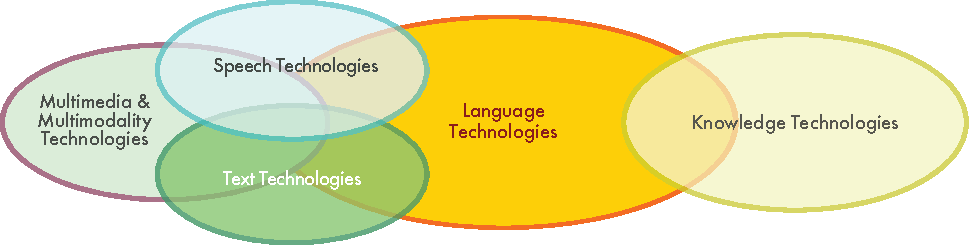
\includegraphics[width=\textwidth]{../_media/english/language_technologies}
  \caption{Language technologies}
  \label{fig:ltincontext_en}
  \colorrule{grey3}{\textwidth}{1.5pt}
\end{figure*}



When we communicate, we combine language with other modes of communication and
information media - for example speaking can involve gestures and facial
expressions. Digital texts link to pictures and sounds. Movies may contain
language in spoken and written form. In other words, speech and text
technologies overlap and interact with other multimodal communication and
multimedia technologies.

In this section, we will discuss the main application areas of language
technology, i.\,e., language checking, web search, speech interaction, and
machine translation. These applications and basic technologies include 


\begin{itemize}
\item spelling correction
\item authoring support
\item computer-assisted language learning
\item information retrieval 
\item information extraction
\item text summarisation
\item question answering
\item speech recognition 
\item speech synthesis 
\end{itemize}


Language technology is an established area of research with an extensive set
of introductory literature. The interested reader is referred to the following
references:  \cite{carstensen-etal1, jurafsky-martin01, manning-schuetze1,
  lt-world1, lt-survey1}.


Before discussing the above application areas, we will shortly describe the
architecture of a typical LT system.



\subsection{Application Architectures}

Software applications for language processing typically consist of several
components that mirror different aspects of language. While such applications
tend to be very complex, Figure~\ref{fig:textprocessingarch_en} shows a 
highly simplified architecture of a typical text processing system. The first 
three modules handle the structure and meaning of the text input:

\begin{enumerate}
\item Pre-processing: cleans the data, analyses or removes formatting, detects
  the input language, detects accents (“citt\`{a}" and “citta'") and apostrophes (“dell'UE" e “della UE") for Italian, and so on.
\item Grammatical analysis: finds the verb, its objects, modifiers and
  other sentence elements; detects the sentence structure.
\item Semantic analysis: performs disambiguation (i.\,e.~, computes the appropriate meaning of words in a given context); resolves anaphora (i.\,e.~, which pronouns refer to which nouns in the sentence) and substitute expressions; represents the meaning of the sentence in a machine-readable way.
\end{enumerate}

After analysing the text, task-specific modules can perform other operations,
such as automatic summarisation and database look-ups.

In the remainder of this section, we firstly introduce the core
application areas for language technology, and follow this with a
brief overview of the state of LT research and education today, and a
description of past and present research programmes. Finally, we
present an expert estimate of core LT tools and resources for Italian
in terms of various dimensions such as availability, maturity and
quality. The general situation of LT for the Italian language is
summarised in figure~\ref{fig:lrlttable_en}
(p.~\pageref{fig:lrlttable_en}) at the end of this chapter. This table
lists all tools and resources that are boldfaced in the text. LT
support for Italian is also compared to other languages that are part
of this series.



\begin{figure*}[htb]
  \colorrule{grey3}{\textwidth}{1.5pt}
  \center
  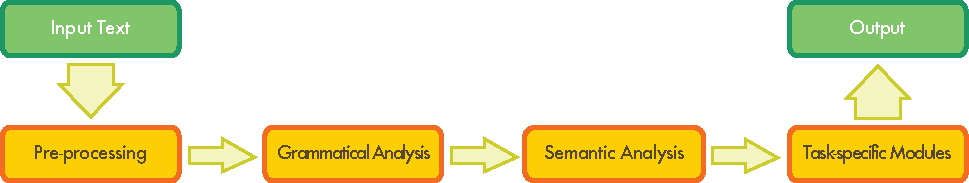
\includegraphics[width=\textwidth]{../_media/english/text_processing_app_architecture}
  \caption{A typical text processing architecture}
  \label{fig:textprocessingarch_en}
  \colorrule{grey3}{\textwidth}{1.5pt}
\end{figure*}



\subsection{Core Application Areas}

In this section, we focus on the most important LT tools and resources, and
provide an overview of LT activities in Italy. 

\subsubsection{Language Checking}

Anyone who has used a word processor such as Microsoft Word knows that it has a spelling checker that highlights spelling mistakes and proposes corrections. The first spelling correction programs compared a list of extracted words against a dictionary of correctly spelled words. Today these programs are far more sophisticated. Using language-dependent algorithms for \textbf{grammatical analysis}, they detect errors related to morphology (e.\,g.~, plural formation) as well as syntax-related errors, such as a missing verb or a conflict of verb-subject agreement (e.\,g.~, \emph{she *write a letter}). However, most spell checkers will not find any errors in the following text: \cite{zar1}:

\begin{quote}
  I have a spelling checker,\\
  It came with my PC.\\
  It plane lee marks four my revue\\
  Miss steaks aye can knot sea.
\end{quote}
 


Handling these kinds of errors usually requires an analysis of the context.
This type of analysis either needs to draw on language-specific
\textbf{grammars} laboriously coded into the software by experts, or on a
statistical language model. In this case, a model calculates the probability
of a particular word as it occurs in a specific position (e.\,g.~, between the
words that precede and follow it). For example: \emph{I can not} is a much more probable word sequence than \emph{aye can knot}. A statistical language model can be automatically created by using a large amount of (correct) language data (called a \textbf{text corpus}). Most of these two approaches have been developed around data from English. Neither approach can transfer easily to Italian because the language has a flexible word order and a richer inflection system. 


\begin{figure*}[htb]
  \colorrule{grey3}{\textwidth}{1.5pt}
  \center
  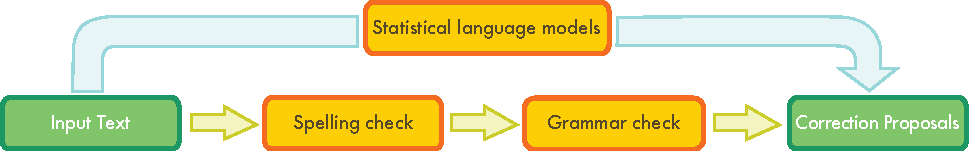
\includegraphics[width=\textwidth]{../_media/english/language_checking}
  \caption{Language checking (top: statistical; bottom: rule-based)}
  \label{fig:langcheckingaarch_en}
  \colorrule{grey3}{\textwidth}{1.5pt}
\end{figure*}


\boxtext{Language checking is not limited to word processors but also applies to authoring systems.}

Language checking is not limited to word processors; it is also used
in authoring support systems, i.\,e., software environments in which
manuals and other types of technical documentation for complex IT,
healthcare, engineering and other products, are written. To offset
customer complaints about incorrect use and damage claims resulting
from poorly understood instructions, companies are increasingly
focusing on the quality of technical documentation while targeting the
international market (via translation or localisation) at the same
time. Advances in natural language processing have led to the
development of authoring support software, which helps the writer of
technical documentation to use vocabulary and sentence structures that
are consistent with industry rules and (corporate) terminology
restrictions.

Besides spell checkers and authoring support, language checking is also important in the field of computer-assisted language learning. And language checking applications also automatically correct search engine queries, as found in Google's \emph{Did you mean...} suggestions.


\subsubsection{Web Search}

\begin{figure*}[htb]
  \colorrule{grey3}{\textwidth}{1.5pt}
  \center
  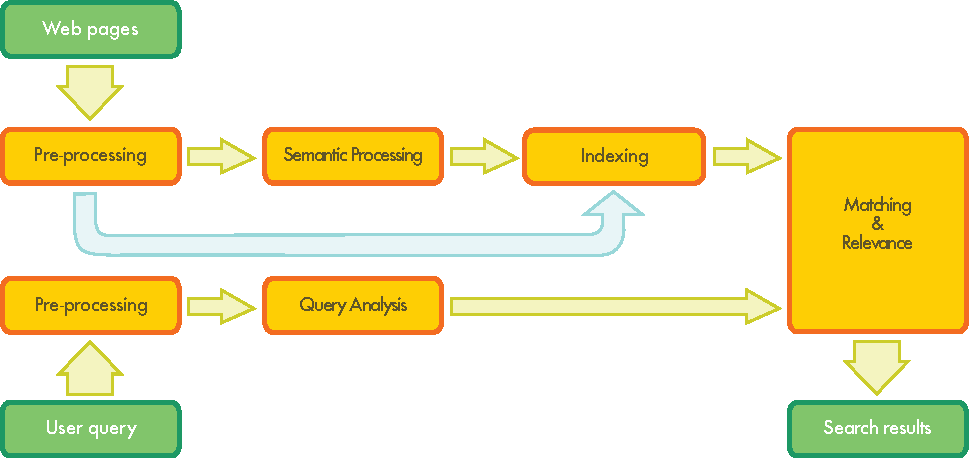
\includegraphics[width=\textwidth]{../_media/english/web_search_architecture}
  \caption{Web search}
  \label{fig:websearcharch_en}
  \colorrule{grey3}{\textwidth}{1.5pt}
 \end{figure*}

Searching the Web, intranets or digital libraries is probably the most widely used yet largely underdeveloped language technology application today. The Google search engine, which started in 1998, now handles about 80\% of all search queries \cite{spi1}. The Google search interface and results page display has not significantly changed since the first version. However, in the current version, Google offers spelling correction for misspelled words and incorporates basic semantic search capabilities that can improve search accuracy by analysing the meaning of terms in a search query context \cite{pc1}. The Google success story shows that a large volume of data and efficient indexing techniques can deliver satisfactory results using a statistical approach to language processing. 

For more sophisticated information requests, it is essential to integrate deeper linguistic knowledge for text interpretation. Experiments using \textbf{lexical resources} such as machine-readable thesauri or ontological language resources (e.\,g.~, WordNet for English or ItalWordNet and MultiWordNet for Italian) have demonstrated improvements in finding pages using synonyms of the original search terms, such as \emph{energia atomica} [atomic energy] and \emph{energia nucleare} [nuclear energy], or even more loosely related terms.


\boxtext{The next generation of search engines\\ will have to include much more
  sophisticated language technology.}


The next generation of search engines will have to include much more
sophisticated language technology, especially to deal with search
queries consisting of a question or other sentence type rather than a
list of keywords. For the query, \textit{Give me a list of all
  companies that were taken over by other companies in the last five
  years}, a syntactic as well as \textbf{semantic analysis} is
required. The system also needs to provide an index to quickly
retrieve relevant documents. A satisfactory answer will require
syntactic parsing to analyse the grammatical structure of the sentence
and determine that the user wants companies that have been acquired,
rather than companies that have acquired other companies. For the
expression \textit{last five years}, the system needs to determine the
relevant range of years, taking into account the present year. The
query then needs to be matched against a huge amount of unstructured
data to find the pieces of information that are relevant to the user’s
request. This process is called information retrieval, and involves
searching and ranking relevant documents. To generate a list of
companies, the system also needs to recognise a particular string of
words in a document represents a company name, using a process called
named entity recognition.


A more demanding challenge is matching a query in one language with
documents in another language. Cross-lingual information retrieval
involves automatically translating the query into all possible source
languages and then translating the results back into the user's target
language.
 
Now that data is increasingly found in non-textual formats, there is a need
for services that deliver multimedia information retrieval by searching
images, audio files and video data. In the case of audio and video files, a
speech recognition module must convert the speech content into text (or into a
phonetic representation) that can then be matched against a user query.

In Italy, among the others, companies like Expert System and CELI successfully develop and apply semantic search technologies.


\subsubsection{Speech Interaction}


Speech interaction is one of many application areas that depend on
speech technology, i.\,e., technologies for processing spoken
language. Speech interaction technology is used to create interfaces
that enable users to interact in spoken language instead of using a
graphical display, keyboard and mouse.  Today, these voice user
interfaces (VUI) are used for partially or fully automated telephone
services provided by companies to customers, employees or
partners. Business domains that rely heavily on VUIs include banking,
supply chain, public transportation, and telecommunications. Other
uses of speech interaction technology include interfaces to car
navigation systems and the use of spoken language as an alternative to
the graphical or touchscreen interfaces in smartphones. Speech
interaction technology comprises four technologies:


\begin{figure*}[htb]
  \colorrule{grey3}{\textwidth}{1.5pt}
  \center
  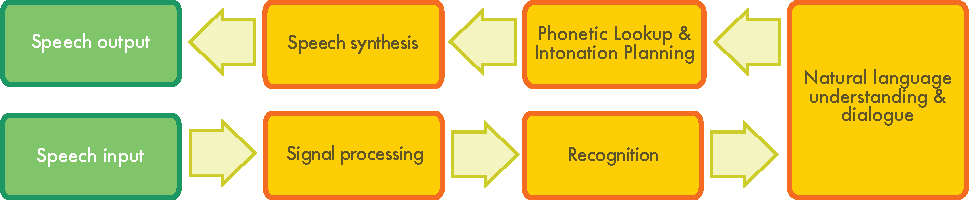
\includegraphics[width=\textwidth]{../_media/english/simple_speech-based_dialogue_architecture}
  \caption{Speech-based dialogue system}
  \label{fig:dialoguearch_en}
  \colorrule{grey3}{\textwidth}{1.5pt}
\end{figure*}


\begin{enumerate}
\item Automatic \textbf{speech recognition} (ASR) determines which words are actually spoken in a given sequence of sounds uttered by a user.
\item Natural language understanding analyses the syntactic structure of a user's utterance and interprets it according to the system in question.
\item Dialogue management determines which action to take given the user input and system functionality.
\item \textbf{Speech synthesis} (text-to-speech or TTS) transforms the
  system's reply into sounds for the user.
\end{enumerate}

One of the major challenges of ASR systems is to accurately recognise the
words a user utters. This means restricting the range of possible user
utterances to a limited set of keywords, or manually creating language models
that cover a large range of natural language utterances. Using machine
learning techniques, language models can also be generated automatically from
\textbf{speech corpora}, i.\,e.~, large collections of speech audio files and
text transcriptions. Restricting utterances usually forces people to use the
voice user interface in a rigid way and can damage user acceptance; but the
creation, tuning and maintenance of rich language models will significantly
increase costs. VUIs that employ language models and initially allow a user to
express their intent more flexibly - prompted by a \emph{How may I help
you?} greeting - tend to be automated and are better accepted by users. 


\boxtext{Speech interaction is the basis for interfaces that allow a user to interact with spoken language.}

Companies tend to use utterances pre-recorded by professional speakers
for generating the output of the voice user interface. For static
utterances where the wording does not depend on particular contexts of
use or personal user data, this can deliver a rich user
experience. But more dynamic content in an utterance may suffer from
unnatural intonation because different parts of audio files have
simply been strung together. Today's TTS systems are getting better
(though they can still be optimised) at producing natural-sounding
dynamic utterances.


Interfaces in speech interaction have been considerably standardised
during the last decade in terms of their various technological
components. There has also been strong market consolidation in speech
recognition and speech synthesis. The national markets in the G20
countries (economically resilient countries with high populations)
have been dominated by just five global players, with Nuance (USA) and
Loquendo (Italy) being the most prominent players in Europe. In 2011,
Nuance announced the acquisition of Loquendo, which represents a
further step in market consolidation.

In the Italian-language ASR market, there are smaller companies such
as PerVoice, Cedat85 and Synthema. With regard to dialogue management
technology and know-how, the market is dominated by national SME
players. In Italy, this includes the IM Service Lab. Rather than
relying on a software license-driven product business, these companies
are mainly positioned as full-service providers that create voice user
interfaces as part of a system integration service. In the area of
interaction technology, there is as yet no real market for syntactic
and semantic analysis-based core technologies.

The demand for voice user interfaces in Italy has grown fast in the last five years, driven by increasing demand for customer self-service, cost optimisation for automated telephone services, and the increasing acceptance of spoken language as a media for human-machine interaction.

Looking ahead, there will be significant changes, due to the spread of smartphones as a new platform for managing customer relationships, in addition to fixed telephones, the Internet and e-mail. This will also affect how speech interaction technology is used. In the long term, there will be fewer telephone-based VUIs, and spoken language apps will play a far more central role as a user-friendly input for smartphones. This will be largely driven by stepwise improvements in the accuracy of speaker-independent speech recognition via the speech dictation services already offered as centralised services to smartphone users.

\subsubsection{Machine Translation}

\begin{figure*}[htb]
  \colorrule{grey3}{\textwidth}{1.5pt}
  \center
  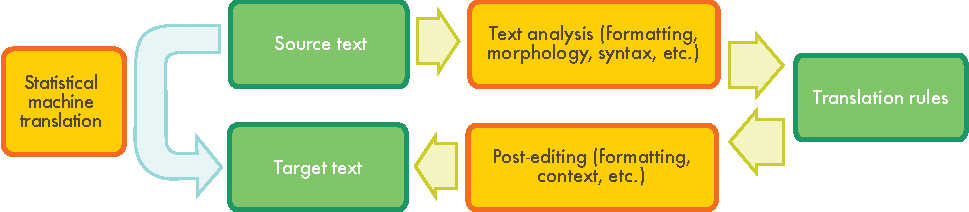
\includegraphics[width=\textwidth]{../_media/english/machine_translation}
  \caption{Machine translation (left: statistical; right: rule-based)}
  \label{fig:mtarch_en}
  \colorrule{grey3}{\textwidth}{1.5pt}
\end{figure*}

The idea of using digital computers to translate natural languages
goes back to 1946 and was followed by substantial funding for research
during the 1950s and again in the 1980s. Yet \textbf{machine
  translation} (MT) still cannot deliver on its initial promise of
providing across-the-board automated translation.  


\boxtext{At its basic level, Machine Translation simply substitutes words in one natural language with words in another language.}

The most basic approach to machine translation is the automatic replacement of the words in a text written in one natural language with the equivalent words of another language. This can be useful in subject domains that have a very restricted, formulaic language such as weather reports.  However, in order to produce a good translation of less restricted texts, larger text units (phrases, sentences, or even whole passages) need to be matched to their closest counterparts in the target language. The major difficulty is that human language is ambiguous. Ambiguity creates challenges on multiple levels, such as word sense disambiguation at the lexical level (a \textit{jaguar} is a brand of car or an animal) or the assignment of case on the syntactic level, for example:

\begin{itemize}
\item The chicken is ready \emph{to eat}.
\item {[}Il pollo  \`{e} pronto \emph{a mangiare}.{]}
\item {[}Il pollo  \`{e} pronto \emph{per essere mangiato}.{]}
\end{itemize}


One way to build an MT system is to use linguistic rules. For translations between closely related languages, a translation using direct substitution may be feasible in cases such as the above example. However, rule-based (or linguistic knowledge-driven) systems often analyse the input text and create an intermediary symbolic representation from which the target language text can be generated. The success of these methods is highly dependent on the availability of extensive lexicons with morphological, syntactic, and semantic information, and large sets of grammar rules carefully designed by skilled linguists. This is a very long and therefore costly process.
 
In the late 1980s when computational power increased and became cheaper, interest in statistical models for machine translation began to grow. Statistical models are derived from analysing bilingual text corpora, \textbf{parallel corpora}, such as the Europarl parallel corpus, which contains the proceedings of the European Parliament in 21 European languages. Given enough data, statistical MT works well enough to derive an approximate meaning of a foreign language text by processing parallel versions and finding plausible patterns of words. Unlike knowledge-driven systems, however, statistical (or data-driven) MT systems often generate ungrammatical output. Data-driven MT is advantageous because less human effort is required, and it can also cover special particularities of the language (e.\,g., idiomatic expressions) that are often ignored in knowledge-driven systems. 

The strengths and weaknesses of knowledge-driven and data-driven machine translation tend to be complementary, so that nowadays researchers focus on hybrid approaches that combine both methodologies. One approach uses both knowledge-driven and data-driven systems together with a selection module that decides on the best output for each sentence. However, results for sentences longer than say 12 words will often be far from perfect. A better solution is to combine the best parts of each sentence from multiple outputs; this can be fairly complex, as corresponding parts of multiple alternatives are not always obvious and need to be aligned. 

\boxtext{Machine Translation is particularly\\ challenging for the Italian language.}

Machine translation is particularly challenging for the Italian language due to the morphological complexity and the free word order of the Italian language. Some companies are active in the MT sector in Italy, mainly providing services for professional usages (for example, Translated).

The use of machine translation can significantly increase productivity
provided that the system is intelligently adapted to user-specific terminology
and integrated into a workflow. Special systems for interactive translation
support were developed.

There is still a huge potential for improving the quality of MT systems. The challenges involve adapting language resources to a given subject domain or user area, and integrating the technology into workflows that already have term bases and translation memories. Another problem is that most of the current systems are English-centred and only support a few languages from and into Italian. This leads to friction in the translation workflow and forces MT users to learn different lexicon coding tools for different systems.

Evaluation campaigns help to compare the quality of MT systems, the different approaches and the status of the systems for different language pairs. Figure~\ref{fig:euromatrix_de} (p.~\pageref{fig:euromatrix_de}), which was prepared during the EC Euromatrix+ project, shows the pair-wise performances obtained for 22 of the 23 official EU languages (Irish was not compared.) The results are ranked according to a BLEU score, which indicates higher scores for better translations \cite{bleu1}. A human translator would achieve a score of around 80 points. 

The best results (in green and blue) were achieved by languages that benefit from a considerable research effort in coordinated programs and from the existence of many parallel corpora (e.\,g.~, English, French, Dutch, Spanish and German). The languages with poorer results are shown in red. These languages either lack such development efforts or are structurally very different from other languages (e.\,g.~, Hungarian, Maltese and Finnish).








% -- \textcolor{grey1}{Machine translation between 22 EU-languages} 


\subsection{Other Application Areas}

Building language technology applications involves a range of subtasks
that do not always surface at the level of interaction with the user,
but they provide significant service functionalities
“behind the scenes” of the system in
question. They all form important research issues that have now
evolved into individual sub-disciplines of computational linguistics. 

Question answering, for example, is an active area of research for which annotated corpora have been built and scientific competitions have been initiated. The concept of question answering goes beyond keyword-based searches (in which the search engine responds by delivering a collection of potentially relevant documents) and enables users to ask a concrete question to which the system provides a single answer. For example:

\begin{itemize}
\item[] \textit{Question: How old was Neil Armstrong when he stepped on the moon?}
\item[] \textit{Answer: 38.}
\end{itemize}

While question answering is obviously related to the core area of web search, it is nowadays an umbrella term for such research issues as which different types of questions exist, and how they should be handled; how a set of documents that potentially contain the answer can be analysed and compared (do they provide conflicting answers?); and how specific information (the answer) can be reliably extracted from a document without ignoring the context. 


\boxtext{Language technology applications often provide significant service functionalities “behind the scenes” of larger software systems.}

Question answering is in turn related to information extraction (IE), an area that was extremely popular and influential when computational linguistics took a statistical turn in the early 1990s. IE aims to identify specific pieces of information in specific classes of documents, such as the key players in company takeovers as reported in newspaper stories. Another common scenario that has been studied is reports on terrorist incidents. The task here consists of mapping appropriate parts of the text to a template that specifies the perpetrator, target, time, location and results of the incident. Domain-specific template-filling is the central characteristic of IE, which makes it another example of a “behind the scenes” technology that forms a well-demarcated research area, which in practice needs to be embedded into a suitable application environment.

Text summarisation and \textbf{text generation} are two borderline areas
that can act either as standalone applications or play a supporting
role. Summarisation attempts to give the essentials of a long text in a short
form, and is one of the features available in Microsoft Word. It mostly uses a
statistical approach to identify the important words in a text (i.\,e.~,
words that occur very frequently in the text in question but less frequently
in general language use) and determine which sentences contain the most of
these important words. These sentences are then extracted and put
together to create the summary.  In this very common commercial scenario, summarisation is simply a form of sentence extraction, and the text is reduced to a subset of its sentences. An alternative approach, for which some research has been carried out, is to generate brand new sentences that do not exist in the source text. 

 
\boxtext{For Italian, research in most text technologies is much less developed than for English.}

This requires a deeper understanding of the text, which means that so
far this approach is far less robust. On the whole, a text generator
is rarely used as a stand-alone application but is embedded into a
larger software environment, such as a clinical information system
that collects, stores and processes patient data. Creating reports is
just one of many applications for text summarisation. 

For the Italian language, research in the text technologies described
above is much less developed than for the English language. Question
answering, information extraction, and summarisation have been the
focus of numerous open competitions in the USA since the 1990s,
primarily organised by the government-sponsored organisations DARPA
and NIST. 

These competitions have significantly improved the state-of-the-art,
but their focus has mostly been on the English language. As a result,
there are fewer annotated corpora or other special resources needed to
perform these tasks in Italian. 

When summarisation systems use purely statistical methods, they are largely language-independent and a number of research prototypes are available. For text generation, reusable components have traditionally been limited to surface realisation modules (generation grammars) and most of the available software is for the English language.


\subsection{Educational Programmes}

Language technology is a very interdisciplinary field that involves
the combined expertise of linguists, computer scientists,
mathematicians, philosophers, psycholinguists, and neuroscientists
among others. As a result, it has not acquired a clear, independent
existence in the Italian faculty system. As for university curricula we mention the second level International Master
on Human Language Technologies and Interface at the University of Trento and
the European Master on Language and Communication Technologies hosted by the
Free University of Bolzano. In addition, according to Libro Bianco at
bachelor, master and PhD level there are at least 16 other curricula related
to HLT (most notably at the Universities of Venice, Turin, Pavia, Pisa, Roma
Tor Vergata, Naples, and Bari), for a total of at least 76 university
courses involving HLT topics, including those related to Humanities Computing curricula.



\subsection{National Projects and Initiatives}

The capability of a language to be “digitally” present in Internet-based applications and services has become a crucial element to maintain the cultural vitality of the language itself. On the other hand, Internet applications and services can be sustained only if adequate infrastructures and technologies are present. As for Italian, the situation cannot be compared to that of English, yet a considerable effort has been invested in Language Technologies research in Italy since 1997, when Human Language Technology (hence forth HLT) was designated a National research policy, with the launch of two three-year projects:


\begin{itemize}
\item TAL, National Infrastructure for Linguistic resources in the field of Automatic Treatment of Spoken and Written Natural Language, funded by the Italian government for about 1.75M Euros;
\item LRCMM, devoted to mono and multilingual research in computational linguistics, funded for about 3M Euros.
\end{itemize}


Funding at the national level is very limited, however. Since the two
projects above were launched, only two small-size projects have been
recently funded, i.\,e.~MIUR-PARLI, for the harmonisation of existing computational resources for Italian, and MIUR-PAIS\`{A} , for the realisation of a platform for learning Italian from annotated corpora.

The majority of the production of language resources and technologies
for Italian is the result of various EU-funded research projects and
other initiatives. 

Thanks to these investments, several lexical
databases as well as spoken and written corpora with both manual and
automatic annotations at different levels (grammatical categories,
syntactic constructions, textual mentions of people, organisations and
locations, etc.) are now available. The same holds true for tools
performing linguistic analysis of Italian, e.\,g.~part of speech taggers, syntactic parsers and named entity recognisers, speech recognition or automatic translation from and into Italian.

Research on HLT is carried on by more than 15 research labs (according to the
EUROMAP study) with an active and relevant presence in the international
research community. Some major events have been organised by the Italian
community, among which the 11\textsuperscript{th} Conference of the European Chapter of the
Association for Computational Linguistics (EACL 2006) in Trento, the 5\textsuperscript{th}
International Conference on Language Resources and Evaluation (LREC 2006) in
Genova and the 12\textsuperscript{th} Annual Conference of the International Speech
Communication Association (Interspeech 2011) in Florence. 

Italian groups are
involved, often with coordination roles, in international networking projects,
particularly at the European Level (for example in CLEF, the Cross Language
Evaluation Forum \cite{clef}, and in FLaReNet, a project fostering an international network for language resources \cite{flarenet}. According to a recent META-NET survey \cite{soria}, there are currently seven national projects running and six European projects coordinated by Italian partners.

Furthermore, 2003 witnessed the founding of CELCT \cite{celct}, the Center for the
Evaluation of Language and Communication Technologies, located in
Trento. Within the Italian Association for Artificial Intelligence
(AI*IA) \cite{aixia}, the special interest group on Natural Language
Processing is the scientific point of reference for the Italian
research community in that field. Italian is included in several
international initiatives for the evaluation of language
technologies. CLEF, for example, has made available comparable tests
in different languages for the organisation of cross language tasks
(e.\,g.~on Question Answering), which include Italian. 

Evalita \cite{evalita}, an evaluation campaign of language technologies devoted exclusively to the Italian language, both spoken and written, has been organised every two years since 2007. The speech community is represented by the Italian Association of Speech Science (AISV) \cite{aisv}. Finally, the Forum Tal \cite{forumtal} plays an important role in the promotion and diffusion of language technologies, in particular in Italian Public Administration, with one of its main achievements being the realisation of the “Libro Bianco” (White Paper) on language technologies in Italy.

In spite of the accomplishments obtained in the field of language
technologies for Italian, the current state of technologies is not
enough to guarantee a digital dimension to Italian such as it is
required by applications and services of the future Internet. For the
coming decades, the Italian community, while also going on with its
effort on basic research, needs to develop technologies for Italian
able to keep up with the size of the data available on the Internet of
the future. In addition, all web-based services will be accessed by
potentially everyone, so the language technologies involved in
providing such services in Italian should support the different
variants of Italian produced by any speaker.



 
\subsection{Availability of Tools and Resources}

Figure~\ref{fig:lrlttable_en} provides a rating for language technology support for the Italian language. This rating of existing tools and resources was generated by leading experts in the field who provided estimates based on a scale from 0 (very low) to 6 (very high) using seven criteria.

\begin{figure*}[htb]
\centering
%\begin{tabular}{>{\columncolor{orange1}}p{.33\linewidth}ccccccc} % ORIGINAL
\begin{tabular}{>{\columncolor{orange1}}p{.33\linewidth}@{\hspace*{6mm}}c@{\hspace*{6mm}}c@{\hspace*{6mm}}c@{\hspace*{6mm}}c@{\hspace*{6mm}}c@{\hspace*{6mm}}c@{\hspace*{6mm}}c}
\rowcolor{orange1}
 \cellcolor{white}&\begin{sideways}\makecell[l]{Quantity}\end{sideways}
&\begin{sideways}\makecell[l]{\makecell[l]{Availability} }\end{sideways} &\begin{sideways}\makecell[l]{Quality}\end{sideways}
&\begin{sideways}\makecell[l]{Coverage}\end{sideways} &\begin{sideways}\makecell[l]{Maturity}\end{sideways} &\begin{sideways}\makecell[l]{Sustainability}\end{sideways} &\begin{sideways}\makecell[l]{Adaptability}\end{sideways} \\ \addlinespace
\multicolumn{8}{>{\columncolor{orange2}}l}{Language Technology: Tools, Technologies and Applications} \\ \addlinespace
Speech Recognition	&2&2&6&5&4.5&3&3 \\ \addlinespace
Speech Synthesis &3&3&5&5&4&3.5&4\\ \addlinespace
Grammatical analysis &3.5&3&4&5&4&3&2\\ \addlinespace
Semantic analysis &2.5&2.5&3.5&4&3&2.5&2.5\\ \addlinespace
Text generation &0&0&0&0&0&0&0\\ \addlinespace
Machine translation &4&3.5&4&3&4&3.5&2.5\\ \addlinespace
\multicolumn{8}{>{\columncolor{orange2}}l}{Language Resources: Resources, Data and Knowledge Bases} \\ \addlinespace
Text corpora &2.5&2.5&4&3.5&3.5&2.5&2\\ \addlinespace
Speech corpora &3&3&4&2.5&2.5&2&2\\ \addlinespace
Parallel corpora &2&2&4&3&4&3&2\\ \addlinespace
Lexical resources &3.5&3.5&5&5&5&2.5&2.5\\ \addlinespace
Grammars &2&2&4&4&3&2&2\\
\end{tabular}
\caption{State of language technology support for Italian}
\label{fig:lrlttable_en}
\end{figure*}




The key results for Italian language technology can be summed up as follows:

\begin{itemize}
\item Speech processing currently seems to be more mature than the processing of written text. In fact, speech technology has already been successfully integrated into many everyday applications, from spoken dialogue systems and voice-based interfaces to mobile phones and car navigation systems. 
\item Research has successfully led to the design of medium to high quality software for basic text analysis, such as tools for morphological analysis and syntactic parsing. But advanced technologies that require deep linguistic processing and semantic knowledge are still in their infancy. 
\item As to resources, there is a large reference text corpus with a balanced mix of genres for the Italian language, but it is difficult to access due to copyright issues; non balanced corpora are easier to access. There are a number of corpora annotated with syntactic, semantic and discourse structure mark-up, but again, there are not nearly enough language corpora containing the right sort of content to meet the growing need for deeper linguistic and semantic information. 
\item In particular, there is a lack of the sort of parallel corpora that form the basis for statistical and hybrid approaches to machine translation. Currently, translation from Italian to English works best because for there are large amounts of parallel text available for this language pair. 
\item Many of these tools, resources and data formats do not meet industry standards and cannot be sustained effectively. A concerted programme is required to standardise data formats and APIs.
\item An unclear legal situation restricts the use of digital texts, e.\,g., those published online by newspapers, for empirical linguistic and language technology research, such as training statistical language models. Together with politicians and policy makers, researchers should try to establish laws or regulations that enable researchers to use publicly available texts for language-related R\&D activities.
\item The cooperation between the Language Technology community and those involved with the Semantic Web and the closely related Linked Open Data movement should be intensified with the goal of establishing a collaboratively maintained, machine-readable knowledge base that can be used both in web-based information systems and as semantic knowledge bases in LT applications. Ideally, this endeavour should be addressed multilingually on the European scale.
\end{itemize}

In a number of specific areas of Italian language research, we have software with limited functionality available today. Obviously, further research efforts are required to meet the current deficit in processing texts on a deeper semantic level and to address the lack of resources such as parallel corpora for machine translation.




\subsection{Cross-language comparison}

The current state of LT support varies considerably from one language community to another. In order to compare the situation between languages, this section will present an evaluation based on two sample application areas (machine translation and speech processing) and one underlying technology (text analysis), as well as basic resources needed for building LT applications. The languages were categorised using the following five-point scale: 

\begin{enumerate}
\item Excellent support
\item Good support
\item Moderate support
\item Fragmentary support
\item Weak or no support
\end{enumerate}


Language Technology support was measured according to the following criteria:

\textbf{Speech Processing:} Quality of existing speech recognition technologies, quality of existing speech synthesis technologies, coverage of domains, number and size of existing speech corpora, amount and variety of available speech-based applications.

\textbf{Machine Translation:} Quality of existing MT technologies, number of language pairs covered, coverage of linguistic phenomena and domains, quality and size of existing parallel corpora, amount and variety of available MT applications.

\textbf{Text Analysis:} Quality and coverage of existing text analysis technologies (morphology, syntax, semantics), coverage of linguistic phenomena and domains, amount and variety of available applications, quality and size of existing (annotated) text corpora, quality and coverage of existing lexical resources (e.\,g., WordNet) and grammars.

\textbf{Resources:} Quality and size of existing text corpora, speech corpora and parallel corpora, quality and coverage of existing lexical resources and grammars.


Figures~\ref{fig:speech_cluster_en} to~\ref{fig:resources_cluster_en} show that, thanks to large-scale LT funding in recent decades, the Italian language is better equipped than most other languages. It compares well with languages with a similar number of speakers, such as German. But LT resources and tools for Italian clearly do not yet reach the quality and coverage of comparable resources and tools for the English language, which is in the lead in almost all LT areas. And there are still plenty of gaps in English language resources with regard to high quality applications.

For speech processing, current technologies perform well enough to be successfully integrated into a number of industrial applications such as spoken dialogue and dictation systems. Today's text analysis components and language resources already cover the linguistic phenomena of Italian to a certain extent and form part of many applications involving mostly shallow natural language processing, e.\,g. spelling correction and authoring support.

However, for building more sophisticated applications, such as machine translation, there is a clear need for resources and technologies that cover a wider range of linguistic aspects and enable a deep semantic analysis of the input text. By improving the quality and coverage of these basic resources and technologies, we shall be able to open up new opportunities for tackling a broader range of advanced application areas, including high-quality machine translation.


\subsection{Conclusions}


\emph{In this series of white papers, we have provided the first high-level comparison of language technology support across 30 European languages.
By identifying the gaps, needs and deficits, the European language technology community and its related stakeholders are now in a position to design a large scale research and development programme aimed at building truly multilingual, technology-enabled communication across Europe.}

The results of this white paper series show that there is a dramatic difference in language technology support between European languages. While there are good quality software and resources available for some languages and application areas, other (usually smaller) languages have substantial gaps. Many languages lack basic technologies for text analysis and the essential resources. \\
Others have basic tools and resources, but there is little chance of implementing semantic methods in the near future. This means that a large-scale effort is needed to reach the ambitious goal of providing support for all European languages, for example through high quality machine translation.

In the case of the Italian language, we can be cautiously optimistic about the current state of language technology support. There is a viable LT research community in Italy, which has been supported in the past by large research programmes. And a number of large-scale resources and state-of-the-art technologies have been produced for Italian. However, the scope of the resources and the range of tools are still very limited when compared to English, and they are simply not sufficient in quality and quantity to develop the kind of technologies required to support a truly multilingual knowledge society.

Nor can we simply transfer technologies already developed and optimised for the English language to handle Italian. English-based systems for parsing (syntactic and grammatical analysis of sentence structure) typically perform far less well on Italian texts, due to the specific characteristics of the Italian language.

The Italian language technology industry is currently fragmented and disorganised. Most large companies have either stopped or severely cut their LT efforts, leaving the field to a number of specialised SMEs that are not robust enough to address the internal and the global market with a sustained strategy. 

Our findings lead to the conclusion that the only way forward is to make a substantial effort to create language technology resources for Italian, as a means to drive forward research, innovation and development. The need for large amounts of data and the extreme complexity of language technology systems makes it vital to develop an infrastructure and a coherent research organisation to spur greater sharing and cooperation.

Finally there is a lack of continuity in research and development funding. Short-term coordinated programmes tend to alternate with periods of sparse or zero funding. In addition, there is an overall lack of coordination with programmes in other EU countries and at the European Commission level.

The long term goal of META-NET is to enable the creation of high-quality language technology for all languages. This requires all stakeholders - in politics, research, business, and society - to unite their efforts. The resulting technology will help tear down existing barriers and build bridges between Europe's languages, paving the way for political and economic unity through cultural diversity. 
\end{multicols}

\begin{figure*}[tb]
  \small
  \centering
  \begin{tabular}
  { % defines color for each column.
  >{\columncolor{corange5}}p{.13\linewidth}@{\hspace{.040\linewidth}}
  >{\columncolor{corange4}}p{.13\linewidth}@{\hspace{.040\linewidth}}
  >{\columncolor{corange3}}p{.13\linewidth}@{\hspace{.040\linewidth}}
  >{\columncolor{corange2}}p{.13\linewidth}@{\hspace{.040\linewidth}}
  >{\columncolor{corange1}}p{.13\linewidth} 
  }
  \multicolumn{1}{>{\columncolor{white}}c@{\hspace{.040\linewidth}}}{\textbf{Excellent}} & 
  \multicolumn{1}{@{}>{\columncolor{white}}c@{\hspace{.040\linewidth}}}{\textbf{Good}} &
  \multicolumn{1}{@{}>{\columncolor{white}}c@{\hspace{.040\linewidth}}}{\textbf{Moderate}} &
  \multicolumn{1}{@{}>{\columncolor{white}}c@{\hspace{.040\linewidth}}}{\textbf{Fragmentary}} &
  \multicolumn{1}{@{}>{\columncolor{white}}c}{\textbf{Weak/no}} \\ 
  \multicolumn{1}{>{\columncolor{white}}c@{\hspace{.040\linewidth}}}{\textbf{support}} & 
  \multicolumn{1}{@{}>{\columncolor{white}}c@{\hspace{.040\linewidth}}}{\textbf{support}} &
  \multicolumn{1}{@{}>{\columncolor{white}}c@{\hspace{.040\linewidth}}}{\textbf{support}} &
  \multicolumn{1}{@{}>{\columncolor{white}}c@{\hspace{.040\linewidth}}}{\textbf{support}} &
  \multicolumn{1}{@{}>{\columncolor{white}}c}{\textbf{support}} \\ \addlinespace
  
& \vspace*{0.5mm}English
& \vspace*{0.5mm}
Czech \newline 
Dutch \newline 
Finnish \newline 
French \newline 
German \newline   
\textbf{Italian} \newline  
Portuguese \newline 
Spanish \newline
& \vspace*{0.5mm}Basque \newline 
Bulgarian \newline 
Catalan \newline 
Danish \newline 
Estonian \newline 
Galician\newline 
Greek \newline  
Hungarian  \newline
Irish \newline  
Norwegian \newline 
Polish \newline 
Serbian \newline 
Slovak \newline 
Slovene \newline 
Swedish \newline
& \vspace*{0.5mm}
Croatian \newline 
Icelandic \newline  
Latvian \newline 
Lithuanian \newline 
Maltese \newline 
Romanian\\
\end{tabular}
\caption{Speech processing: state of language technology support for 30 European languages}
\label{fig:speech_cluster_en}
\end{figure*}

\begin{figure*}[tb]
  \small
  \centering
  \begin{tabular}
  { % defines color for each column.
  >{\columncolor{corange5}}p{.13\linewidth}@{\hspace{.040\linewidth}}
  >{\columncolor{corange4}}p{.13\linewidth}@{\hspace{.040\linewidth}}
  >{\columncolor{corange3}}p{.13\linewidth}@{\hspace{.040\linewidth}}
  >{\columncolor{corange2}}p{.13\linewidth}@{\hspace{.040\linewidth}}
  >{\columncolor{corange1}}p{.13\linewidth} 
  }
  \multicolumn{1}{>{\columncolor{white}}c@{\hspace{.040\linewidth}}}{\textbf{Excellent}} & 
  \multicolumn{1}{@{}>{\columncolor{white}}c@{\hspace{.040\linewidth}}}{\textbf{Good}} &
  \multicolumn{1}{@{}>{\columncolor{white}}c@{\hspace{.040\linewidth}}}{\textbf{Moderate}} &
  \multicolumn{1}{@{}>{\columncolor{white}}c@{\hspace{.040\linewidth}}}{\textbf{Fragmentary}} &
  \multicolumn{1}{@{}>{\columncolor{white}}c}{\textbf{Weak/no}} \\ 
  \multicolumn{1}{>{\columncolor{white}}c@{\hspace{.040\linewidth}}}{\textbf{support}} & 
  \multicolumn{1}{@{}>{\columncolor{white}}c@{\hspace{.040\linewidth}}}{\textbf{support}} &
  \multicolumn{1}{@{}>{\columncolor{white}}c@{\hspace{.040\linewidth}}}{\textbf{support}} &
  \multicolumn{1}{@{}>{\columncolor{white}}c@{\hspace{.040\linewidth}}}{\textbf{support}} &
  \multicolumn{1}{@{}>{\columncolor{white}}c}{\textbf{support}} \\ \addlinespace
  
& \vspace*{0.5mm} English 
& \vspace*{0.5mm} 
French \newline 
Spanish
& \vspace*{0.5mm}
Catalan \newline 
Dutch \newline 
German \newline 
Hungarian \newline
\textbf{Italian} \newline 
Polish \newline 
Romanian \newline 
& \vspace*{0.5mm}Basque \newline 
Bulgarian \newline 
Croatian \newline 
Czech \newline
Danish \newline 
Estonian \newline 
Finnish \newline 
Galician \newline 
Greek \newline 
Icelandic \newline 
Irish \newline 
Latvian \newline 
Lithuanian \newline 
Maltese \newline 
Norwegian \newline 
Portuguese \newline 
Serbian \newline 
Slovak \newline 
Slovene \newline 
Swedish \newline 
\end{tabular}
\caption{Machine translation: state of language technology support for 30 European languages}
\label{fig:mt_cluster_en}
\end{figure*}

\begin{figure*}[tb]
  \small
  \centering
  \begin{tabular}
  { % defines color for each column.
  >{\columncolor{corange5}}p{.13\linewidth}@{\hspace{.040\linewidth}}
  >{\columncolor{corange4}}p{.13\linewidth}@{\hspace{.040\linewidth}}
  >{\columncolor{corange3}}p{.13\linewidth}@{\hspace{.040\linewidth}}
  >{\columncolor{corange2}}p{.13\linewidth}@{\hspace{.040\linewidth}}
  >{\columncolor{corange1}}p{.13\linewidth} 
  }
  \multicolumn{1}{>{\columncolor{white}}c@{\hspace{.040\linewidth}}}{\textbf{Excellent}} & 
  \multicolumn{1}{@{}>{\columncolor{white}}c@{\hspace{.040\linewidth}}}{\textbf{Good}} &
  \multicolumn{1}{@{}>{\columncolor{white}}c@{\hspace{.040\linewidth}}}{\textbf{Moderate}} &
  \multicolumn{1}{@{}>{\columncolor{white}}c@{\hspace{.040\linewidth}}}{\textbf{Fragmentary}} &
  \multicolumn{1}{@{}>{\columncolor{white}}c}{\textbf{Weak/no}} \\ 
  \multicolumn{1}{>{\columncolor{white}}c@{\hspace{.040\linewidth}}}{\textbf{support}} & 
  \multicolumn{1}{@{}>{\columncolor{white}}c@{\hspace{.040\linewidth}}}{\textbf{support}} &
  \multicolumn{1}{@{}>{\columncolor{white}}c@{\hspace{.040\linewidth}}}{\textbf{support}} &
  \multicolumn{1}{@{}>{\columncolor{white}}c@{\hspace{.040\linewidth}}}{\textbf{support}} &
  \multicolumn{1}{@{}>{\columncolor{white}}c}{\textbf{support}} \\ \addlinespace

& \vspace*{0.5mm}English
& \vspace*{0.5mm}
  Dutch \newline 
  French \newline 
  German \newline 
  \textbf{Italian} \newline 
  Spanish
& \vspace*{0.5mm}Basque \newline 
  Bulgarian \newline 
  Catalan \newline 
  Czech \newline 
  Danish \newline 
  Finnish \newline 
  Galician \newline 
  Greek \newline 
  Hungarian \newline 
  Norwegian \newline 
  Polish \newline 
  Portuguese \newline 
  Romanian \newline 
  Slovak \newline 
  Slovene \newline 
  Swedish \newline 
& \vspace*{0.5mm}
  Croatian \newline 
  Estonian \newline 
  Icelandic \newline 
  Irish \newline 
  Latvian \newline 
  Lithuanian \newline 
  Maltese \newline 
  Serbian \\
  \end{tabular}
\caption{Text analysis: state of language technology support for 30 European languages}
\label{fig:text_cluster_en}
\end{figure*}

\begin{figure*}[tb]
  \small
  \centering
  \begin{tabular}
  { % defines color for each column.
  >{\columncolor{corange5}}p{.13\linewidth}@{\hspace{.040\linewidth}}
  >{\columncolor{corange4}}p{.13\linewidth}@{\hspace{.040\linewidth}}
  >{\columncolor{corange3}}p{.13\linewidth}@{\hspace{.040\linewidth}}
  >{\columncolor{corange2}}p{.13\linewidth}@{\hspace{.040\linewidth}}
  >{\columncolor{corange1}}p{.13\linewidth} 
  }
  \multicolumn{1}{>{\columncolor{white}}c@{\hspace{.040\linewidth}}}{\textbf{Excellent}} & 
  \multicolumn{1}{@{}>{\columncolor{white}}c@{\hspace{.040\linewidth}}}{\textbf{Good}} &
  \multicolumn{1}{@{}>{\columncolor{white}}c@{\hspace{.040\linewidth}}}{\textbf{Moderate}} &
  \multicolumn{1}{@{}>{\columncolor{white}}c@{\hspace{.040\linewidth}}}{\textbf{Fragmentary}} &
  \multicolumn{1}{@{}>{\columncolor{white}}c}{\textbf{Weak/no}} \\ 
  \multicolumn{1}{>{\columncolor{white}}c@{\hspace{.040\linewidth}}}{\textbf{support}} & 
  \multicolumn{1}{@{}>{\columncolor{white}}c@{\hspace{.040\linewidth}}}{\textbf{support}} &
  \multicolumn{1}{@{}>{\columncolor{white}}c@{\hspace{.040\linewidth}}}{\textbf{support}} &
  \multicolumn{1}{@{}>{\columncolor{white}}c@{\hspace{.040\linewidth}}}{\textbf{support}} &
  \multicolumn{1}{@{}>{\columncolor{white}}c}{\textbf{support}} \\ \addlinespace
    
& \vspace*{0.5mm}English
& \vspace*{0.5mm} 
    Czech \newline 
    Dutch \newline 
    French \newline 
    German \newline 
    Hungarian \newline
    \textbf{Italian} \newline
    Polish \newline
    Spanish \newline
    Swedish \newline 
& \vspace*{0.5mm} Basque\newline 
    Bulgarian\newline 
    Catalan \newline 
    Croatian \newline 
    Danish \newline 
    Estonian \newline 
    Finnish \newline 
    Galician \newline 
    Greek \newline 
    Norwegian \newline 
    Portuguese \newline 
    Romanian \newline 
    Serbian \newline 
    Slovak \newline 
    Slovene \newline
&  \vspace*{0.5mm}
    Icelandic \newline 
    Irish \newline 
    Latvian \newline 
    Lithuanian \newline 
    Maltese  \\
  \end{tabular}
  \caption{Speech and text resources: state of support for 30 European languages}  
  \label{fig:resources_cluster_en}
\end{figure*}


\clearpage

\ssection[About META-NET]{About META-NET}

\begin{multicols}{2}

META-NET is a Network of Excellence partially funded by the European Commission \cite{rehm2011}. The network currently consists of 54 research centres in 33 European countries. META-NET forges META, the Multilingual Europe Technology Alliance, a growing community of language technology professionals and organisations in Europe. META-NET fosters the technological foundations for a truly multilingual European information society that:

\begin{itemize}
\item makes communication and cooperation possible across languages;
\item grants all Europeans equal access to information and knowledge regardless of their language;
\item builds upon and advances functionalities of networked information technology.
\end{itemize}

The network supports a Europe that unites as a single digital market and information space. It stimulates and promotes multilingual technologies for all European languages. These technologies support automatic translation, content production, information processing and knowledge management for a wide variety of subject domains and applications. They also enable intuitive language-based interfaces to technology ranging from household electronics, machinery and vehicles to computers and robots.
Launched on 1 February 2010, META-NET has already conducted various activities in its three lines of action META-VISION, META-SHARE and META-RESEARCH.

\textbf{META-VISION} fosters a dynamic and influential stakeholder community that unites around a shared vision and a common strategic research agenda (SRA). The main focus of this activity is to build a coherent and cohesive LT community in Europe by bringing together representatives from highly fragmented and diverse groups of stakeholders. The present White Paper was prepared together with volumes for 29 other languages. The shared technology vision was developed in three sectorial Vision Groups. The META Technology Council was established in order to discuss and to prepare the SRA based on the vision in close interaction with the entire LT community.

\textbf{META-SHARE} creates an open, distributed facility for exchanging and sharing resources. The peer-to-peer network of repositories will contain language data, tools and web services that are documented with high-quality metadata and organised in standardised categories. The resources can be readily accessed and uniformly searched. The available resources include free, open source materials as well as restricted, commercially available, fee-based items.

\textbf{META-RESEARCH} builds bridges to related technology fields. This activity seeks to leverage advances in other fields and to capitalise on innovative research that can benefit language technology. In particular, the action line focuses on conducting leading-edge research in machine translation, collecting data, preparing data sets and organising language resources for evaluation purposes; compiling inventories of tools and methods; and organising workshops and training events for members of the community.\\\\

\textbf{\centerline{office@meta-net.eu -- http://www.meta-net.eu}}
\end{multicols}

\cleardoublepage

\appendix
\addtocontents{toc}{\protect\bigskip}

\bsection[Riferimenti bibliografici -- References]{Riferimenti bibliografici --- References}
\bibliographystyle{unsrt}
\bibliography{italian_references}
  
\cleardoublepage

\bsection[Membri di META-NET -- META-NET Members]{Membri di META-NET --- META-NET Members}
\label{metanetmembers}

\small
\begin{longtable}{llp{110mm}}
  
  Austria & \textcolor{grey1}{Austria} & Zentrum für Translationswissenschaft, Universität Wien: Gerhard Budin\\ \addlinespace 
  Belgio & \textcolor{grey1}{Belgium} & Computational Linguistics and Psycholinguistics Research Centre, University of Antwerp: Walter Daelemans\\ \addlinespace
  & & Centre for Processing Speech and Images, University of Leuven:\newline Dirk van Compernolle \\ \addlinespace
  Bulgaria & \textcolor{grey1}{Bulgaria} & Inst. for Bulgarian Language, Bulgarian Academy of Sciences: Svetla Koeva \\ \addlinespace
  Cipro & \textcolor{grey1}{Cyprus} & Language Centre, School of Humanities: Jack Burston \\ \addlinespace
  Croazia & \textcolor{grey1}{Croatia} & Inst. of Linguistics, Faculty of Humanities and Social Science, University of Zagreb: Marko Tadić \\ \addlinespace
  Danimarca &  \textcolor{grey1}{Denmark} & Centre for Language Technology, University of Copenhagen:\newline Bolette Sandford Pedersen, Bente Maegaard\\ \addlinespace
  Estonia & \textcolor{grey1}{Estonia} & Inst. of Computer Science, University of Tartu: Tiit Roosmaa, Kadri Vider\\ \addlinespace
  Finlandia & \textcolor{grey1}{Finland} & Computational Cognitive Systems Research Group, Aalto University:\newline Timo Honkela\\ \addlinespace
  & & Department of Modern Languages, University of Helsinki: Kimmo Koskenniemi, Krister Lindén \\ \addlinespace
  Francia & \textcolor{grey1}{France} & Centre National de la Recherche Scientifique, Laboratoire d'Informatique pour la Mécanique et les Sciences de l'Ingénieur and Inst. for Multilingual and Multimedia Information: Joseph Mariani \\ \addlinespace
  & & Evaluations and Language Resources Distribution Agency: Khalid Choukri\\ \addlinespace 
  Germania & \textcolor{grey1}{Germany} & Language Technology Lab, DFKI: Hans Uszkoreit, Georg Rehm\\ \addlinespace
  & & Human Language Technology and Pattern Recognition, RWTH Aachen University: Hermann Ney \\ \addlinespace
  & & Department of Computational Linguistics, Saarland University: Manfred Pinkal\\ \addlinespace 
  Grecia & \textcolor{grey1}{Greece} & R.C. “Athena”, Inst. for Language and Speech Processing: Stelios Piperidis\\ \addlinespace
  Irlanda & \textcolor{grey1}{Ireland} & School of Computing, Dublin City University: Josef van Genabith\\ \addlinespace
  Islanda & \textcolor{grey1}{Iceland} & School of Humanities, University of Iceland: Eiríkur Rögnvaldsson\\ \addlinespace
  Italia & \textcolor{grey1}{Italy} & Consiglio Nazionale delle Ricerche, Istituto di Linguistica Computazionale “Antonio Zampolli”: Nicoletta Calzolari\\ \addlinespace
  & & Human Language Technology Research Unit, Fondazione Bruno Kessler:\newline Bernardo Magnini\\ \addlinespace 
  Lettonia & \textcolor{grey1}{Latvia} & Tilde: Andrejs Vasiļjevs\\ \addlinespace 
  & & Inst. of Mathematics and Computer Science, University of Latvia: Inguna Skadiņa\\ \addlinespace
  Lituania & \textcolor{grey1}{Lithuania} & Inst. of the Lithuanian Language: Jolanta Zabarskaitė\\ \addlinespace
  Lussemburgo & \textcolor{grey1}{Luxembourg} & Arax Ltd.: Vartkes Goetcherian\\ \addlinespace
  Malta & \textcolor{grey1}{Malta} & Department Intelligent Computer Systems, University of Malta: Mike Rosner\\ \addlinespace
  Norvegia & \textcolor{grey1}{Norway} & Department of Linguistic,
  Literary and Aesthetic Studies, University of Bergen: Koenraad De Smedt\\ \addlinespace 
  & & Department of Informatics, Language Technology Group, University of Oslo: Stephan Oepen \\ \addlinespace
  Paesi Bassi & \textcolor{grey1}{Netherlands} & Utrecht Inst. of Linguistics, Utrecht University: Jan Odijk\\ \addlinespace 
  & & Computational Linguistics, University of Groningen: Gertjan van Noord\\ \addlinespace
  Polonia & \textcolor{grey1}{Poland} & Inst. of Computer Science, Polish Academy of Sciences: Adam Przepiórkowski,\newline Maciej Ogrodniczuk \\ \addlinespace
  & & University of Łódź: Barbara Lewandowska-Tomaszczyk, Piotr Pęzik\\ \addlinespace
  & & Department of Computer Linguistics and Artificial Intelligence, Adam Mickiewicz University: Zygmunt Vetulani \\ \addlinespace
  Portogallo & \textcolor{grey1}{Portugal} & University of Lisbon: António Branco, Amália Mendes \\ \addlinespace
  & & Spoken Language Systems Laboratory, Inst. for Systems Engineering and Computers: Isabel Trancoso \\ \addlinespace
  Regno Unito & \textcolor{grey1}{UK} & 
  School of Computer Science, University of Manchester: Sophia Ananiadou \\ \addlinespace 
  & & Inst. for Language, Cognition and Computation, Centre for Speech Technology Research, University of Edinburgh: Steve Renals \\ \addlinespace 
  & & Research Inst. of Informatics and Language Processing, University of Wolverhampton: Ruslan Mitkov \\ \addlinespace 
  Repubblica Ceca & \textcolor{grey1}{Czech Republic} & Inst. of Formal and Applied Linguistics, Charles University in Prague: Jan Hajič \\ \addlinespace
  Romania & \textcolor{grey1}{Romania} & Research Inst. for Artificial Intelligence, Romanian Academy of Sciences: Dan Tufiș \\ \addlinespace
  & & Faculty of Computer Science, University Alexandru Ioan Cuza of Iași: Dan Cristea \\ \addlinespace
  Serbia & \textcolor{grey1}{Serbia} & University of Belgrade, Faculty of Mathematics: Duško Vitas, Cvetana Krstev,\newline Ivan Obradović \\ \addlinespace
  & & Pupin Inst.: Sanja Vranes \\ \addlinespace  
  Slovacchia & \textcolor{grey1}{Slovakia} &  Ľudovít Štúr Inst. of Linguistics, Slovak Academy of Sciences: Radovan Garabík \\ \addlinespace 
  Slovenia & \textcolor{grey1}{Slovenia} & Jožef Stefan Inst.: Marko Grobelnik \\ \addlinespace 
  Spagna & \textcolor{grey1}{Spain} & Barcelona Media: Toni Badia, Maite Melero \\ \addlinespace 
  & & Institut Universitari de Lingüística Aplicada, Universitat Pompeu Fabra: Núria Bel \\ \addlinespace 
  & & Aholab Signal Processing Laboratory, University of the Basque Country:\newline Inma Hernaez Rioja \\ \addlinespace 
  & & Center for Language and Speech Technologies and Applications, Universitat Politècnica de Catalunya:  Asunción Moreno \\ \addlinespace 
  & & Department of Signal Processing and Communications, University of Vigo:\newline Carmen García Mateo \\ \addlinespace 
  Svezia & \textcolor{grey1}{Sweden} & Department of Swedish, University of Gothenburg: Lars Borin \\ \addlinespace 
  Svizzera & \textcolor{grey1}{Switzerland} & Idiap Research Inst.: Hervé Bourlard \\ \addlinespace 
  Ungheria & \textcolor{grey1}{Hungary} & Research Inst. for Linguistics, Hungarian Academy of Sciences: Tamás Váradi\\  \addlinespace
  & & Department of Telecommunications and Media Informatics, Budapest University of Technology and Economics: Géza Németh, Gábor Olaszy\\ \addlinespace

\end{longtable}
\normalsize

\renewcommand*{\figureformat}{}
\renewcommand*{\captionformat}{}

\begin{figure*}[htbp]
  \colorrule{grey3}{\textwidth}{1.5pt}
  \center
  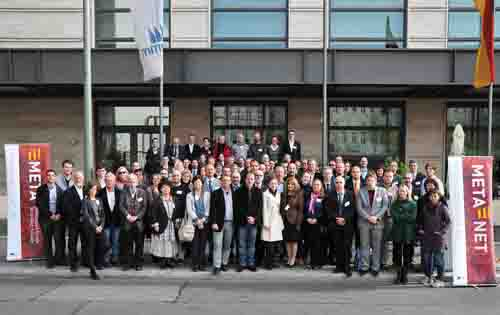
\includegraphics[width=\textwidth]{../_media/meta-net_team.jpg}
   %\fbox{Dummy -- we'll include the group photo of our META-NET meeting in Berlin here}
  \caption{Quasi 100 esperti di tecnologie linguistiche - in rappresentanza dei paesi e delle lingue rappresentate in META-NET - hanno discusso e messo a punto i principali messaggi e risultati della Collana Libri Bianchi durante una riunione di META-NET a Berlino, Germania, il 21 e 22 ottobre 2011. --- \textcolor{grey1}{About 100 language technology experts -- representatives of the countries and languages represented in META-NET -- discussed and finalised the key results and messages of the White Paper Series at a META-NET meeting in Berlin, Germany, on October 21/22, 2011.}}
  \medskip
  \colorrule{grey3}{\textwidth}{1.5pt}
\end{figure*}

\cleardoublepage

\bsection[La Collana Libri Bianchi META-NET -- The META-NET White Paper Series]{La Collana Libri Bianchi META-NET --- The META-NET\ \ \ \ \ \ White Paper Series}
\label{whitepaperseries}

\vspace*{-5mm}
\centering
  \setlength{\tabcolsep}{2em}
  \begin{tabularx}{\textwidth}{lllll} \toprule\addlinespace
  %\begin{tabulary}{170mm}{LLL} \toprule
  Basco & Basque & euskara\\
  Bulgaro & Bulgarian & български\\
  Catalano & Catalan & català \\
  Ceco & Czech & čeština\\
  Croato & Croatian & hrvatski\\
  Danese & Danish & dansk\\
  Estone & Estonian & eesti\\
  Finlandese & Finnish & suomi\\
  Francese & French & français\\
  Galiziano & Galician & galego\\
  Greco & Greek & ελληνικά\\
  Inglese & English & English\\
  Irlandese & Irish & Gaeilge\\
  Islandese & Icelandic & íslenska\\
  Italiano & Italian & italiano\\
  Lettone & Latvian & latviešu valoda\\
  Lituano & Lithuanian & lietuvių kalba\\
  Maltese & Maltese & Malti\\
  Norvegese Bokmål & Norwegian Bokmål & bokmål\\
  Norvegese Nynorsk & Norwegian Nynorsk & nynorsk\\
  Olandese & Dutch & Nederlands\\
  Polacco & Polish & polski\\
  Portoghese & Portuguese & português\\
  Rumeno & Romanian & română\\
  Serbo & Serbian & српски\\
  Slovacco & Slovak & slovenčina\\
  Sloveno & Slovene & slovenščina\\
  Spagnolo & Spanish & español\\
  Svedese & Swedish & svenska\\
  Tedesco & German & Deutsch\\
  Ungherese & Hungarian & magyar\\ \addlinespace \bottomrule
\end{tabularx}
